

\newpage
\appendix 
\begin{subappendices}

\section{Terminology Tables}
\label{TerminologyAppendix}

\subsection{Section \ref{TerminologySection}: General Terminology}
\makebox[\textwidth][c]{
\begin{tabular}{ l l l }
Name & Symbol & Short Description\\
\hline 
Graph & $G$ & \\
Node set & $V$ & \\
Edge set & $E$ & \\
Path & $(v_1, \cdots , v_k)$ & List of nodes connected by edges \\
Residual path &  & A path where all edges have $r(u, v) > 0$ \\
Augmenting path &  & A residual path from $s$ to $t$ \\
Bounding edge &  & The edges in a residual path that have  \\
&&minimum residual capacity\\
Capacity & $cap(u, v)$ & Maximum flow that can be sent on an edge \\
Maximum capacity & $U$ & $\max\limits_{(u, v)\in E}cap(u, v)$ \\
Flow & $f(u, v)$ & The flow sent on an edge \\
Residual capacity& $r(u, v)$ & The amount of flow that can be sent \\
&&without exceeding $cap$\\
Residual Edge & & An edge where the residual capacity replaces the capacity\\
Edge set & $E_f$ & The set of residual edges of $E$ based on flow $f$\\
Residual Graph &$G_f$& $G_f = (V,E_f)$\\
An Eligeble edge & & Has positive residual capacity\\
Saturated edge& & An edge where $r(u, v) = 0$ \\
Distance& $distance(u, v)$ & Number of edges in the shortest \\
&&residual path connecting $u$ to $v$\\
Excess & $e(v)$ & The sum of flow entering a node $v$, \\
&&minus the sum of flow exiting it.\\
\hline
\end{tabular}
}

\subsection{Section \ref{ParadigmsSection}: Paradigms}
\makebox[\textwidth][c]{
\begin{tabular}{ l l l }
Name & Symbol & Short Description\\
\hline 
Blocking flow & &\\
Layer Graph  & &\\
Push, Relabel  & &\\
Label  & $d(v)$ & The label of a node $v$. Used by Push-Relable algorithms.\\
\hline
\end{tabular}
}

\subsection{Section \ref{GoldbergTarjanSection}: A. V. Goldberg R. E. Tarjan 1988}
\makebox[\textwidth][c]{
\begin{tabular}{ l l }
Symbol & Short Description\\
\hline 
Eligible & An edge $(v,w)$ is eligible if it has $r(v,w) > 0$\\
Active & A node $v$ is active if $e(v) > 0$\\
Current-edge & The edge the algorithm would try to push on next. \\
&Also the edge linked in the Dynamic Tree data structure\\
Saturating push & A push operation on an edge that used all the residual capacity \\
Pass & Pass $i+1$ consist of working on all the nodes that was put in the queue at pass $i$\\
Large & A dynamic tree $T$ is large if $|T| \geq k/2$\\
\hline
\end{tabular}
}

\subsection{Section \ref{KRGameSection}: King Rao 1992 - The Game}
\makebox[\textwidth][c]{
\begin{tabular}{ l l }
Symbol & Short Description\\
\hline 
$G_g=(U_g, V_g, E_g)$ & A bipartite graph used in the game\\
$N=|U_g|=|V_g|$ & The number of nodes in the game graph.\\
$M=|E_g|$ & The number of edges in the game graph.\\
$P(N, M)$ & A function that specifies a bound on how   \\
& many points the adversary can obtain.\\
$C(N, M)$ & A function that specifies a bound on the \\
& cost of implementing the player's strategy.\\
$r_0$ & Determines when a node changes ratio level.\\
$r_i=2^ir_0$ & \\
$t$ & The highest ratio level allowed is $r_t$.\\
$l$ & Nodes with fewer edges than the parameter $l$\\
& can use any edge as the designated edge.\\
$U_g'=\{u \in U_g \mid \mathrm{degree}(u) > l\}$ & The nodes in $U_g$ that has degree greater than $l$.\\
$r(v)=\frac{\mathrm{degree_{designated}}(v)}{\mathrm{degree_{initial}}(v)}$ & The ratio of the node $v \in V_g$.\\
$rl(v)=\left\{
\begin{aligned}
0 &\text{ if }r(v)<r_0\\
i &\text{ if }r_i \leq r(v)< r_{i+1}\\
t &\text{ if }r_t \leq r(v)
\end{aligned}
\right.$ & The ratio level of the node $v \in V_g$.\\
$erl(v)\in [rl(v), rl(v)+1]$ & The estimated ratio level of the node $v \in V_g$\\
$V_i=\left\{v\in V_g\mid rl(v) \geq i\right\}$ & \\
$U_i$ & Nodes in $U_g'$ whose designated edge go to a node in $V_i$. \\
\hline
\end{tabular}
}

\subsection{Section \ref{KRGameAnalysisSection}: King Rao 1992 - Analysis of The Game}
\makebox[\textwidth][c]{
\begin{tabular}{ l l }
Symbol & Short Description\\
\hline 
$U_i(v)$ & The nodes in $U_i$ whose designated edge go to $v$.\\
\hline
\end{tabular}
}

\subsection{Section \ref{KRAlgorithmSection}: King Rao 1992 - The Algorithm}
\makebox[\textwidth][c]{
\begin{tabular}{ l l }
Symbol & Short Description\\
\hline 
$E^*\subseteq E$ & The edges that are added to the graph\\
$h(v)=\sum\limits_{(v, u)\in E\setminus E^*}{cap(v, u)}$ & The hidden capacity of a node.\\
$e^*(v)=max\left(0, e(v)-h(v)\right)$ & The visible excess of a node. A node is not allowed to\\
& push more flow away from it than its visible excess.\\
\hline
\end{tabular}
}

\subsection{Section \ref{GRSection}: A. V. Goldberg S. Rao 1998}
\makebox[\textwidth][c]{
\begin{tabular}{ l l }
Symbol & Short Description\\
\hline 
$\Lambda = \min{\{n^{\frac{2}{3}},m^{\frac{1}{2}}\}}$ & \\
$\Delta=\frac{F}{\Lambda}$ & Bounds which edges are admissible\\
$d(v)$ & The distance label of a node $v$\\
$ l(v,w)$ & Length function. Zero iff $r(v,w) \geq 2\Delta$\\
Special edge $(v,w)$ & $\Delta \leq r(v,w) \leq 2\Delta, d(v) = d(w), r(w,v) \geq 2\Delta$\\
$ \bar{l}(v,w)$ & Length function. Zero if special edge or $r(v,w) \geq 2\Delta$\\
Admissible & An edge $(v,w)$ is admissible if $d(v) = \bar{l}(v,w) + d(w)$ and $r(v,w)>0$\\
$F$ & Upper bound on the remaining flow that can be sent.\\
 & It is updated to capacities of cuts in the graph.\\
Iteration & One iteration is one sequence of constructing a layer graph,\\
& running the blocking flow algorithm and routing flow in SSCs.\\
Phase & One phase is a series of iterations resulting in an update to $F$\\
\hline
\end{tabular}
}


\subsection{Algorithm Abbriviations}
\label{AlgorithmAbbrivationsSection}
\makebox[\textwidth][c]{
\begin{tabular}{|l|c|c|c|c|}
    Abbriviation & Dynamic Trees & Low Memory & Global Relabeling Trigger & Library \\\hline\hline
    \multicolumn{5}{|c|}{\textbf{Edmonds and Karp}} \\\hline
    EK &&&&\\\hline
    EK Lib&&&&$\times$\\\hline\hline
    \multicolumn{5}{|c|}{\textbf{Dinic}} \\\hline
    Dinic &&&&\\\hline\hline
    \multicolumn{5}{|c|}{\textbf{Goldberg and Tarjan}} \\\hline
    GT &&&&\\\hline
    GT GRC &&&Cycle&\\\hline
    GT GRP &&&Pass&\\\hline
    GT GRN &&&Node Count&\\\hline
    GT D&$\times$&&&\\\hline
    GT D GRC &$\times$&&Cycle&\\\hline
    GT D GRP &$\times$&&Pass&\\\hline
    GT D GRN &$\times$&&Node Count&\\\hline
    GT Lib&&&&$\times$\\\hline\hline
    \multicolumn{5}{|c|}{\textbf{King and Rao}} \\\hline
    KR D&$\times$&&&\\\hline
    KR D GRC&$\times$&&Cycle&\\\hline
    KR D GRP&$\times$&&Pass&\\\hline
    KR LM&&$\times$&&\\\hline
    KR LM GRC&&$\times$&Cycle&\\\hline
    KR LM GRP&&$\times$&Pass&\\\hline
    KR LM GRN&&$\times$&Node Count&\\\hline
    KR LM D&$\times$&$\times$&&\\\hline
    KR LM D GRC&$\times$&$\times$&Cycle&\\\hline
    KR LM D GRP&$\times$&$\times$&Pass&\\\hline
    KR LM D GRN&$\times$&$\times$&Node Count&\\\hline\hline
    \multicolumn{5}{|c|}{\textbf{Goldberg and Rao}} \\\hline
    GR&$\times$&&&\\\hline\hline
    \multicolumn{5}{|c|}{\textbf{Boykov and Kolmogorov}} \\\hline
    BK Lib&&&&$\times$\\\hline
\end{tabular}
}


\subsection{Global Relabeling Node count trigger functions}
\label{GRN_Functions}
\makebox[\textwidth][c]{
\begin{tabular}{|l|c|c|}
    \hline
    Algorithm & Function & $R^2$ \\\hline\hline
    GT GRN&$f(G)=2.018n^{0.6488}$&$0.946$\\\hline
    GT D GRN&$f(G)=0.5281n^{0.7145}$&$0.9325$\\\hline
    KR LM GRN&$f(G)=2.1674n^{0.7244}$&$0.7766$\\\hline
    KR LM D GRN&$f(G)=11.649n^{0.4249}$&$0.1684$\\\hline
\end{tabular}
}

\begin{figure}[h]
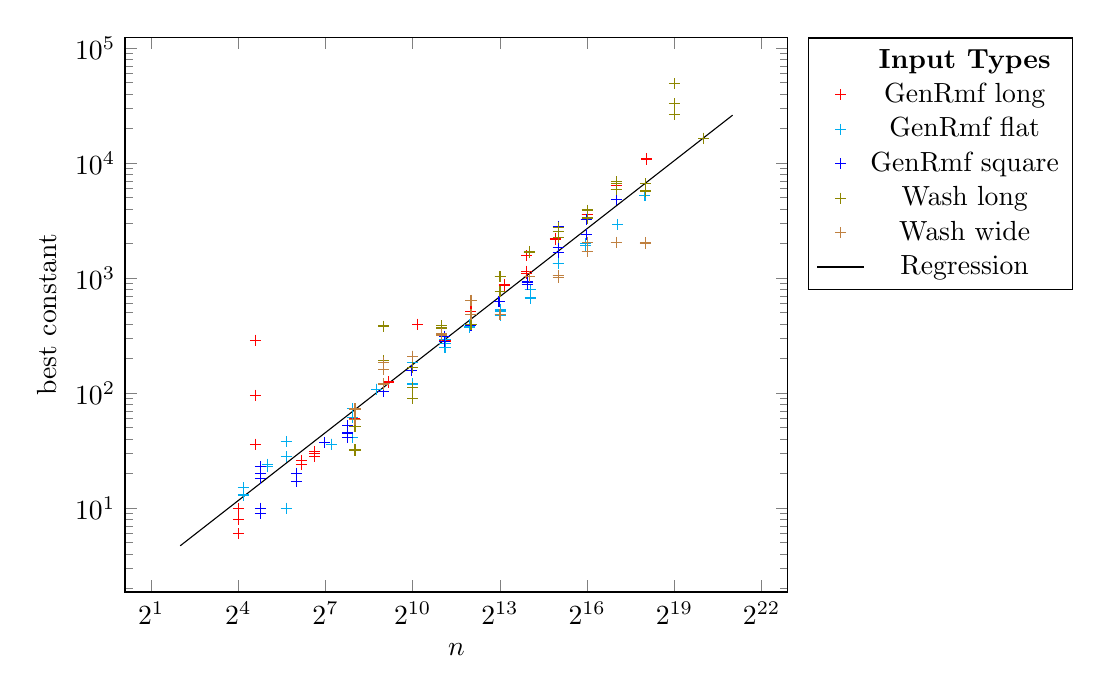
\begin{tikzpicture}
\begin{axis}[
    xlabel=$n$,ylabel=best constant,
    xmode=log,ymode=log,
    log basis x={2},
    legend style=
    {
        legend pos=outer north east
    },
    width=10cm
]
\addlegendimage{legend image code/.code=}
\legend{\textbf{Input Types}, GenRmf long, GenRmf flat, GenRmf square, Wash long, Wash wide, Regression}
\addplot [mark=+, red, only marks]table[x=n,y=value] {%GenRmf long
n   value
16	6
24	96
72	26
99	31
256	60
575	123
1152	396
2205	284
4096	512
9100	864
15488	1565
30589	2206
65536	3584
130682	5869
270848	10712
16	10
24	36
72	24
99	28
256	60
575	125
1152	396
2205	284
4096	512
9100	878
15488	1149
30589	2149
65536	3584
130682	6380
270848	10712
16	8
24	289
72	24
99	30
256	60
575	125
1152	396
2205	281
4096	512
9100	868
15488	1089
30589	2206
65536	3584
130682	5901
270848	10922
};
\addplot [mark=+, cyan, only marks]table[x=n,y=value] {%GenRmf flat
n   value
18	15
32	23
50	28
147	36
243	41
432	108
1024	184
2205	292
3920	380
8214	517
16807	795
32768	1344
63504	1937
135531	2908
259308	5218
18	13
32	24
50	38
147	36
243	61
432	108
1024	120
2205	272
3920	374
8214	533
16807	795
32768	1344
63504	1987
135531	2908
259308	5218
18	15
32	24
50	10
147	36
243	73
432	108
1024	184
2205	250
3920	397
8214	476
16807	671
32768	1344
63504	1987
135531	2908
};
\addplot [mark=+, blue, only marks]table[x=n,y=value] {%GenRmf square
n   value
27	20
27	23
64	20
125	37
216	52
512	104
1000	156
2197	309
4096	385
8000	625
15625	884
32768	1841
64000	3234
132651	4789
27	9
27	9
64	17
125	37
216	41
512	104
1000	156
2197	312
4096	384
8000	625
15625	933
32768	1680
64000	3234
132651	4792
27	10
27	18
64	20
125	37
216	45
512	104
1000	156
2197	282
4096	384
8000	625
15625	916
32768	2816
64000	2375
132651	4792
};
\addplot [mark=+, olive, only marks]table[x=n,y=value] {%Wash long
n   value
258	32
514	192
1026	168
2050	368
4098	480
8194	1024
16386	1673
32770	2752
65538	3344
131074	6880
262146	6592
524290	32768
1048578	16384
258	51
514	191
1026	112
2050	368
4098	480
8194	768
16386	1707
32770	2536
65538	3909
131074	5887
262146	5631
524290	49152
1048578	16512
258	32
514	383
1026	90
2050	384
4098	392
8194	1028
16386	1664
32770	2268
65538	3328
131074	6646
262146	5744
524290	26640
1048578	16512
};
\addplot [mark=+, brown, only marks]table[x=n,y=value] {%Wash wide
n   value
258	73
514	120
1026	209
2050	325
4098	480
8194	481
16386	1024
32770	1052
65538	2046
131074	2048
262146	1984
258	72
514	160
1026	209
2050	316
4098	480
8194	480
16386	1026
32770	1052
65538	1696
131074	2048
262146	1984
258	59
514	184
1026	209
2050	328
4098	640
8194	480
16386	1024
32770	1016
65538	1696
131074	2048
262146	2048
};
\addplot [domain=4:2097152]{1.8956*x^0.6548};
\end{axis}
\end{tikzpicture}
\caption{Constant estimation for Global Relabel with node count trigger for Goldberg Tarjan (GT GRN)}
\label{fig:GT_GRN_Constant}
\end{figure}

\begin{figure}[h]
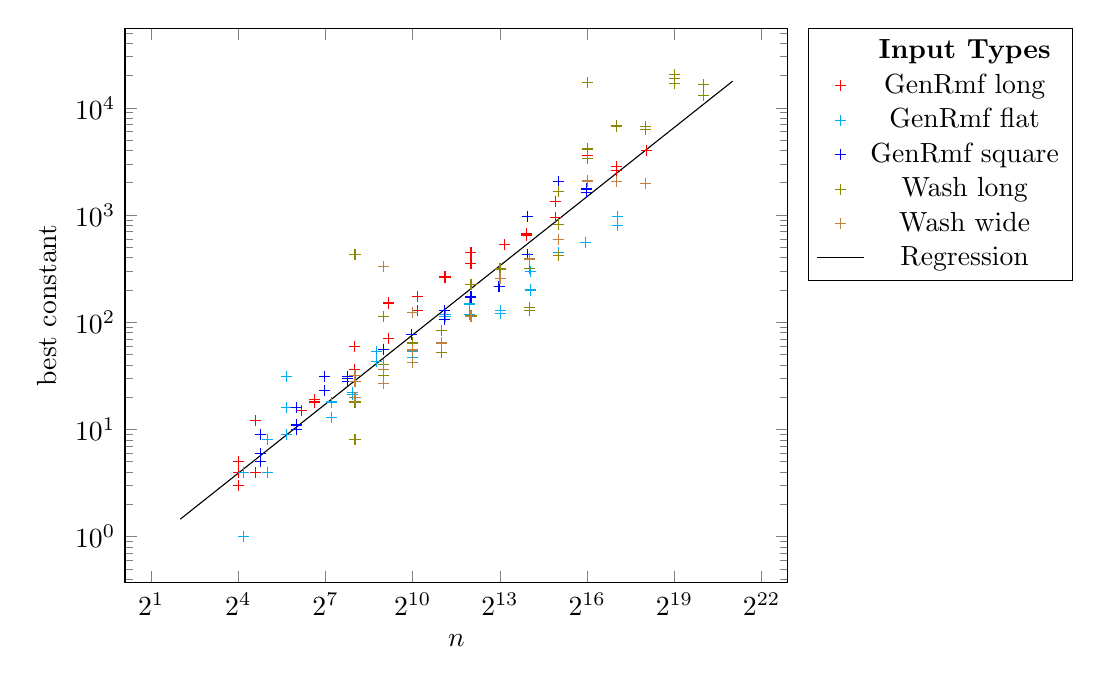
\begin{tikzpicture}
\begin{axis}[
    xlabel=$n$,ylabel=best constant,
    xmode=log,ymode=log,
    log basis x={2},
    legend style=
    {
        legend pos=outer north east
    },
    width=10cm
]
\addlegendimage{legend image code/.code=}
\legend{\textbf{Input Types}, GenRmf long, GenRmf flat, GenRmf square, Wash long, Wash wide, Regression}
\addplot [mark=+, red, only marks]table[x=n,y=value] {%GenRmf long
n   value
16	4
24	4
72	15
99	18
256	59
575	71
1152	175
2205	264
4096	352
9100	532
15488	650
30589	1327
65536	3584
130682	2582
270848	4020
16	5
24	4
72	15
99	18
256	36
575	151
1152	175
2205	264
4096	352
9100	532
15488	650
30589	1327
65536	3584
130682	2809
270848	4020
16	3
24	12
72	15
99	19
256	36
575	71
1152	129
2205	265
4096	448
9100	532
15488	665
30589	940
65536	3584
130682	2614
270848	3983
};
\addplot [mark=+, cyan, only marks]table[x=n,y=value] {%GenRmf flat
n   value
18	4
32	4
50	9
147	18
243	22
432	43
1024	53
2205	119
3920	148
8214	120
16807	200
32768	444
63504	558
135531	801
32	8
50	31
147	18
243	21
432	53
1024	47
2205	114
3920	118
8214	120
16807	196
32768	444
63504	558
135531	800
18	1
32	4
50	16
147	13
243	21
432	43
1024	53
2205	112
3920	118
8214	128
16807	296
32768	444
63504	558
135531	966
};
\addplot [mark=+, blue, only marks]table[x=n,y=value] {%GenRmf square
n   value
27	5
27	5
64	10
125	23
216	30
512	56
1000	77
2197	106
4096	172
8000	216
15625	427
32768	2040
64000	1624
27	5
27	5
64	16
125	23
216	31
512	56
1000	77
2197	128
4096	172
8000	216
15625	427
32768	2040
64000	1750
27	6
27	9
64	11
125	31
216	28
512	56
1000	77
2197	128
4096	172
8000	216
15625	976
32768	2048
64000	1750
};
\addplot [mark=+, olive, only marks]table[x=n,y=value] {%Wash long
n   value
258	429
514	40
1026	64
2050	52
4098	112
8194	318
16386	136
32770	812
65538	3344
131074	6648
262146	6752
524290	18656
1048578	16512
258	8
514	112
1026	64
2050	84
4098	116
8194	313
16386	128
32770	1664
65538	4128
131074	6880
262146	6656
524290	16704
1048578	12928
258	18
514	32
1026	64
2050	52
4098	223
8194	320
16386	320
32770	416
65538	17289
131074	6678
262146	6272
524290	20480
1048578	16384
};
\addplot [mark=+, brown, only marks]table[x=n,y=value] {%Wash wide
n   value
258	20
514	27
1026	124
2050	64
4098	112
8194	256
16386	392
32770	592
65538	2112
131074	2048
262146	1984
258	28
514	333
1026	42
2050	64
4098	112
8194	256
16386	384
32770	588
65538	2112
131074	2048
262146	1984
258	32
514	36
1026	55
2050	64
4098	113
8194	256
16386	384
32770	592
65538	2047
131074	2048
262146	1984
};
\addplot [domain=4:2097152]{0.54*x^0.7144};
\end{axis}
\end{tikzpicture}
\caption{Constant estimation for Global Relabel with node count trigger for Goldberg Tarjan Dynamic (GT D GRN)}
\label{fig:GT_D_GRN_Constant}
\end{figure}



\begin{figure}[h]
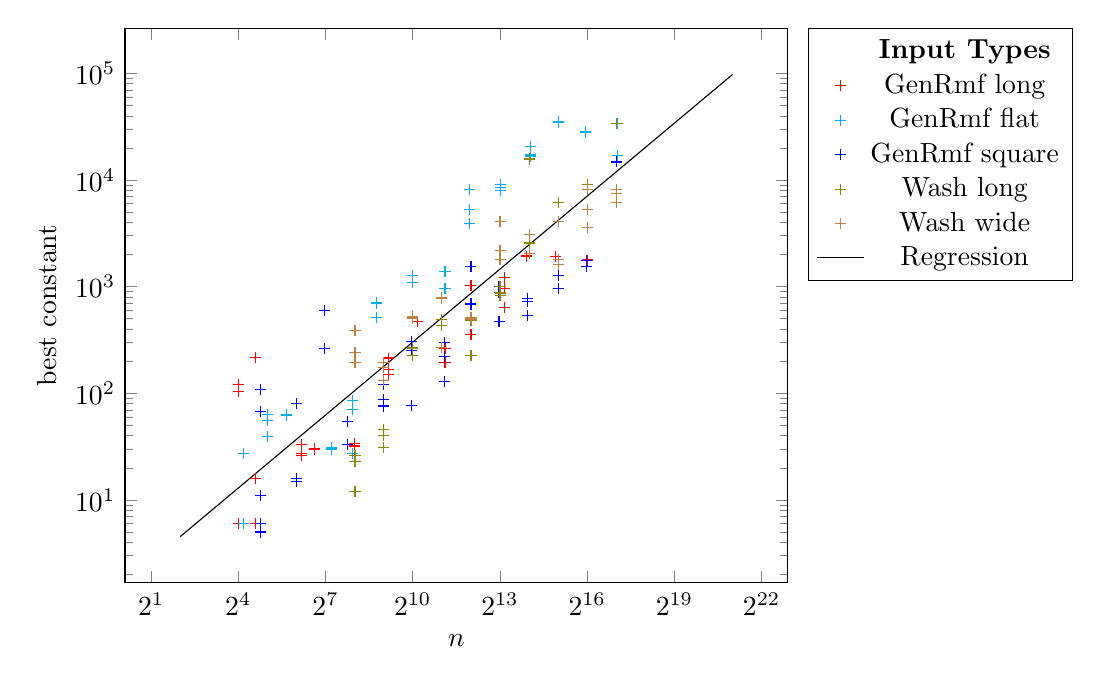
\begin{tikzpicture}
\begin{axis}[
    xlabel=$n$,ylabel=best constant,
    xmode=log,ymode=log,
    log basis x={2},
    legend style=
    {
        legend pos=outer north east
    },
    width=10cm
]
\addlegendimage{legend image code/.code=}
\legend{\textbf{Input Types}, GenRmf long, GenRmf flat, GenRmf square, Wash long, Wash wide, Regression}
\addplot [mark=+, red, only marks]table[x=n,y=value] {%GenRmf long
n   value
16	6
24	217
72	33
99	30
256	34
575	151
1152	468
2205	261
4096	1024
9100	643
15488	1928
30589	1911
65536	1776
16	121
24	16
72	27
99	30
256	32
575	214
1152	468
2205	261
4096	356
9100	960
15488	1928
30589	1911
65536	1776
16	104
24	6
72	26
99	30
256	32
575	167
1152	468
2205	196
4096	1024
9100	1208
15488	1936
30589	1911
65536	1776
};
\addplot [mark=+, cyan, only marks]table[x=n,y=value] {%GenRmf flat
n   value
18	6
32	39
50	62
147	30
243	86
432	702
1024	1092
2205	964
3920	5259
8214	8426
16807	20421
32768	34712
63504	28775
135531	16941
18	27
32	63
50	63
147	31
243	27
432	708
1024	1276
2205	1377
3920	3896
8214	9111
16807	16807
32768	35300
63504	27783
135531	33882	
32	56
50	62
147	30
243	71
432	509
1024	1276
2205	966
3920	8085
8214	7961
16807	17332
32768	35332
63504	28771
135531	16941
};
\addplot [mark=+, blue, only marks]table[x=n,y=value] {%GenRmf square
n   value
27	108
64	15	
216	33
512	88
1000	305
2197	299
4096	687
8000	875
15625	537
32768	960
64000	1765
132651	14768
27	6
27	11
64	80
125	265
216	54
512	76
1000	77
2197	222	
8000	468
15625	732
32768	952
64000	1531
132651	14767
27	5
27	67
64	16
125	598
216	33
512	120
1000	250
2197	128
4096	1552
8000	1000
15625	777
32768	1280
64000	1765
132651	14768
};
\addplot [mark=+, olive, only marks]table[x=n,y=value] {%Wash long
n   value
258	23
514	40
1026	228
2050	495
4098	483
8194	871
16386	2560
32770	6209
65538	9092
131074	33792
258	26
514	31
1026	228
2050	432
4098	224
8194	832
16386	2584
32770	6209
65538	9094
131074	33792
258	12
514	46
1026	266
2050	433
4098	482
8194	1006
16386	15753
32770	6172
65538	9094
131074	33728
};
\addplot [mark=+, brown, only marks]table[x=n,y=value] {%Wash wide
n   value
258	240
514	174
1026	513
2050	787
4098	498
8194	1797
16386	3080
32770	1600
65538	5248
131074	8160
258	385
514	132
1026	500
2050	270
4098	496
8194	4075
16386	2048
32770	1792
65538	8192
131074	7480
258	196
514	196
1026	522
2050	767
4098	512
8194	2179
16386	2054
32770	4066
65538	3584
131074	6147
};
\addplot [domain=4:2097152]{1.5834*x^0.7578};
\end{axis}
\end{tikzpicture}
\caption{Constant estimation for Global Relabel with node count trigger for King Rao Low Memory (GT LM GRN)}
\label{fig:KR LM_GRN_Constant}
\end{figure}



\begin{figure}[h]
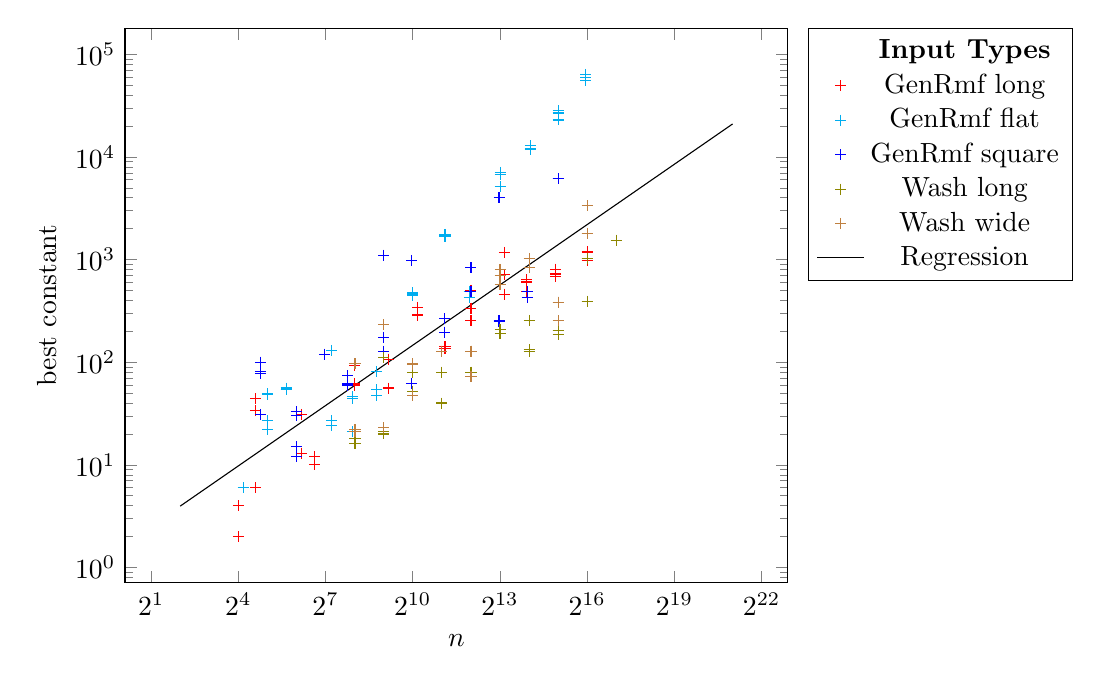
\begin{tikzpicture}
\begin{axis}[
    xlabel=$n$,ylabel=best constant,
    xmode=log,ymode=log,
    log basis x={2},
    legend style=
    {
        legend pos=outer north east
    },
    width=10cm
]
\addlegendimage{legend image code/.code=}
\legend{\textbf{Input Types}, GenRmf long, GenRmf flat, GenRmf square, Wash long, Wash wide, Regression}
\addplot [mark=+, red, only marks]table[x=n,y=value] {%GenRmf long
n   value
24	44
72	13
99	10
256	92
575	107
1152	288
2205	141
4096	336
9100	1172
15488	635
30589	804
65536	1184
16	4
24	34
72	13
99	12
256	60
575	107
1152	342
2205	141
4096	254
9100	711
15488	605
30589	681
65536	1029
16	2
24	6
72	31
99	10
256	62
575	56
1152	290
2205	137
4096	501
9100	461
15488	484
30589	723
65536	972
};
\addplot [mark=+, cyan, only marks]table[x=n,y=value] {%GenRmf flat
n   value
18	6
32	27
50	54
147	27
243	44
432	47
1024	456
2205	1756
3920	490
8214	5133
16807	11782
32768	26752
63504	55806
18	6
32	22
50	54
147	24
243	46
432	81
1024	448
2205	1684
3920	490
8214	7056
16807	12079
32768	28288
63504	59535
18	6
32	49
50	56
147	130
243	21
432	54
1024	472
2205	1703
3920	426
8214	6673
16807	12876
32768	22896
63504	63566
};
\addplot [mark=+, blue, only marks]table[x=n,y=value] {%GenRmf square
n   value
27	81
64	15	
216	74
512	175
1000	62
2197	196
4096	832
8000	255
15625	488
32768	6144	
27	77
64	12	
216	60
512	128
1000	62
2197	196
4096	832
8000	250
15625	431
32768	6144	
27	100
64	30
27	31
64	33
125	120
216	62
512	1102
1000	979
2197	265
4096	488
8000	4032
};
\addplot [mark=+, olive, only marks]table[x=n,y=value] {%Wash long
n   value
258	18
514	20
1026	52
2050	80
4098	80
8194	207
16386	132
32770	204
65538	392
131074	1536
258	16
514	21
1026	52
2050	40
4098	73
8194	191
16386	256
32770	204
65538	392
131074	1540	
514	111
1026	80	
4098	73	
16386	128
32770	188
65538	1024
131074	1536
};
\addplot [mark=+, brown, only marks]table[x=n,y=value] {%Wash wide
n   value
258	22
514	23
1026	96
2050	128
4098	73
8194	800
16386	1016
32770	384
65538	1796
258	21
514	23
1026	96
2050	128
4098	128
8194	577
16386	836
32770	384
65538	1792
258	97
514	232
1026	47
2050	128
4098	128
8194	704
16386	832
32770	254
65538	3336
};
\addplot [domain=4:2097152]{1.6078*x^0.6509};
\end{axis}
\end{tikzpicture}
\caption{Constant estimation for Global Relabel with node count trigger for King Rao Low Memory Dynamic (KR LM D GRN)}
\label{fig:KR_LM_GRN_Constant}
\end{figure}

    
\clearpage
\section{Charts}
\label{ChartAppendix}


\subsection{Results from CRH graphs}
\begin{figure}[h]
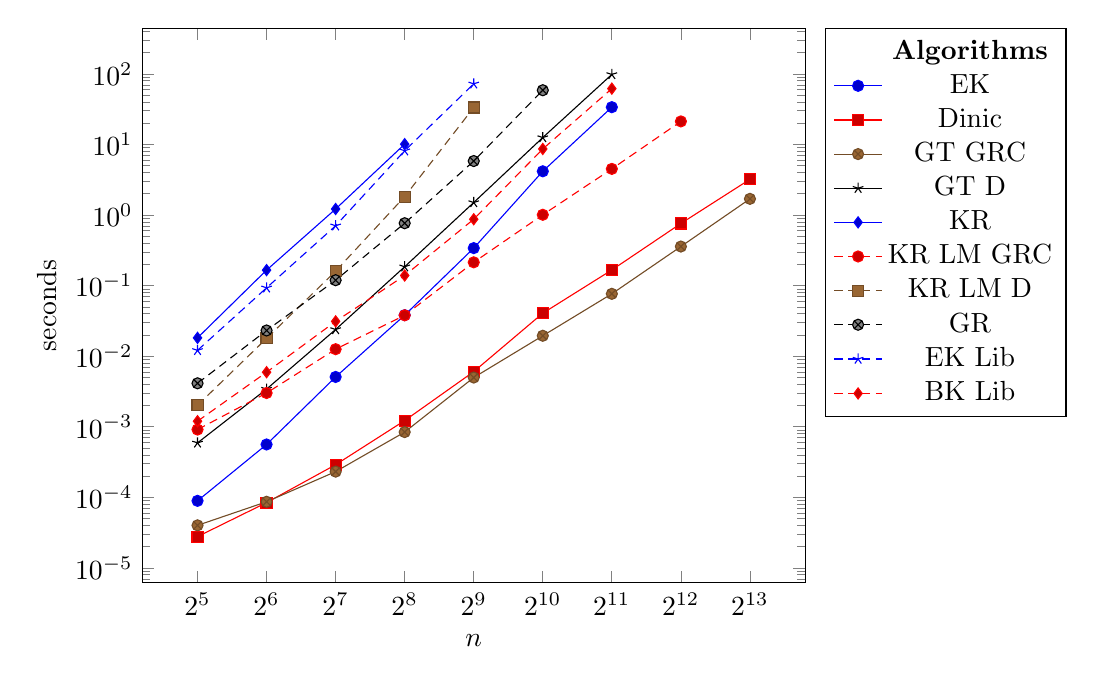
\begin{tikzpicture}
\begin{axis}[
    xlabel=$n$,ylabel=seconds,
    xmode=log,ymode=log,
    log basis x={2},
    legend style=
    {
        legend pos=outer north east
    },
    width=10cm
]
\addlegendimage{legend image code/.code=}
\legend{\textbf{Algorithms}, EK, Dinic, GT GRC, GT D, KR, KR LM GRC, KR LM D, GR, EK Lib, BK Lib}
\addplot table[x=n,y=value] {%EK
n value
32	8.91727E-05
64	0.00056091
128	0.005077953
256	0.038123333
512	0.339550667
1024	4.16451
2048	33.72456667
};
\addplot table[x=n,y=value] {%Dinic
n value
32	2.77623E-05
64	8.41754E-05
128	0.000289727
256	0.001222433
512	0.006034197
1024	0.040603633
2048	0.166434667
4096	0.758745667
8192	3.204413333
};
\addplot table[x=n,y=value] {%GT GRC
n value
32	4.00888E-05
64	8.65074E-05
128	0.000231315
256	0.000840643
512	0.004980787
1024	0.019460933
2048	0.0764499
4096	0.357635
8192	1.694086667
};
\addplot table[x=n,y=value] {%GT D
n value
32	0.000590562
64	0.003415777
128	0.023887433
256	0.185035333
512	1.504396667
1024	12.51486667
2048	98.09486667
};
\addplot table[x=n,y=value] {%KR
n value
32	0.0181733
64	0.165739667
128	1.21656
256	10.09223333
};
\addplot table[x=n,y=value] {%KR LM GRC
n value
32	0.000912274
64	0.00300656
128	0.012558933
256	0.037942
512	0.213656667
1024	1.007368333
2048	4.502716667
4096	21.199
};
\addplot table[x=n,y=value] {%KR LM D
n value
32	0.002014107
64	0.017856
128	0.16025
256	1.82407
512	33.37643333
};
\addplot table[x=n,y=value] {%GR
n value
32	0.004126927
64	0.023131233
128	0.119142333
256	0.765221333
512	5.817686667
1024	58.60563333
};
\addplot table[x=n,y=value] {%EK Lib
n value
32	0.0120941
64	0.092989167
128	0.704491333
256	8.1467
512	72.2544
};
\addplot table[x=n,y=value] {%BK Lib
n value
32	0.001199007
64	0.00592652
128	0.031122567
256	0.138813
512	0.871689667
1024	8.632126667
2048	61.7279
};
\end{axis}
\end{tikzpicture}
\caption{Best and worst results from the CRH graphs}
\label{fig:CRH_BW_Results}
\end{figure}


\begin{figure}[h]
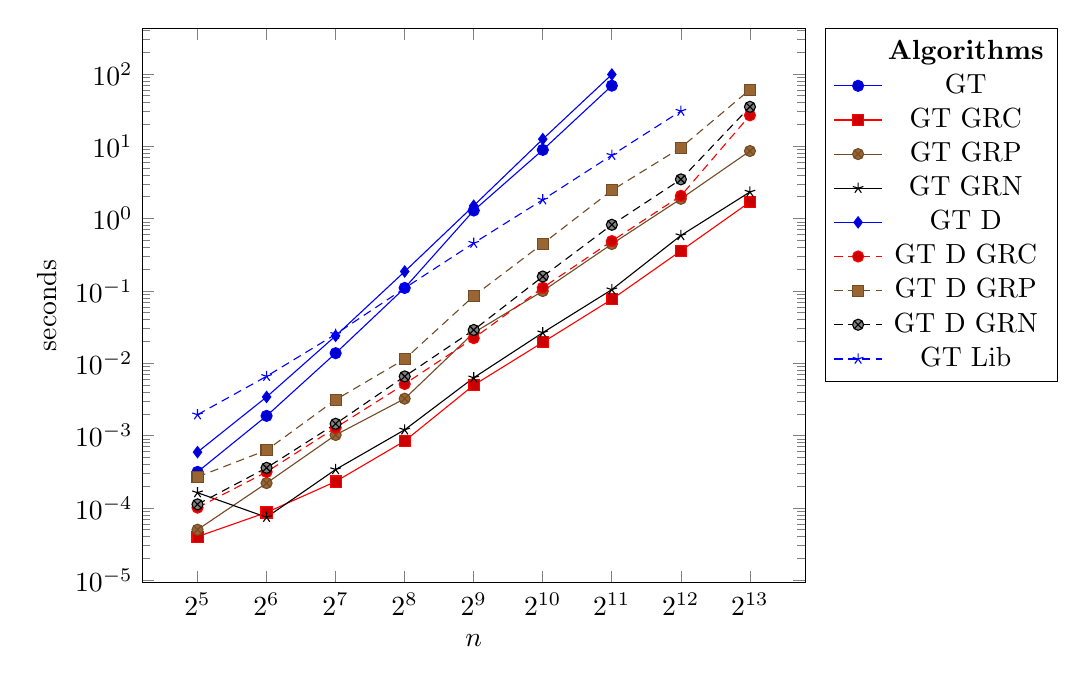
\begin{tikzpicture}
\begin{axis}[
    xlabel=$n$,ylabel=seconds,
    xmode=log,ymode=log,
    log basis x={2},
    legend style=
    {
        legend pos=outer north east
    },
    width=10cm
]
\addlegendimage{legend image code/.code=}
\legend{\textbf{Algorithms}, GT, GT GRC, GT GRP, GT GRN, GT D, GT D GRC, GT D GRP, GT D GRN, GT Lib}
\addplot table[x=n,y=value] {%GT
n value
32	0.000314492
64	0.001870183
128	0.0137617
256	0.109700333
512	1.290522
1024	8.888233333
2048	68.60676667
};
\addplot table[x=n,y=value] {%GT GRC
n value
32	4.00888E-05
64	8.65074E-05
128	0.000231315
256	0.000840643
512	0.004980787
1024	0.019460933
2048	0.0764499
4096	0.357635
8192	1.694086667
};
\addplot table[x=n,y=value] {%GT GRP
n value
32	4.99722E-05
64	0.000220322
128	0.0010181
256	0.003234533
512	0.026379533
1024	0.0994381
2048	0.444045
4096	1.873073333
8192	8.57279
};
\addplot table[x=n,y=value] {%GT GRN
n value
32	0.000162244
64	7.41812E-05
128	0.000339257
256	0.00120067
512	0.00629929
1024	0.0264405
2048	0.104068667
4096	0.582426667
8192	2.32921
};
\addplot table[x=n,y=value] {%GT D
n value
32	0.000590562
64	0.003415777
128	0.023887433
256	0.185035333
512	1.504396667
1024	12.51486667
2048	98.09486667
};
\addplot table[x=n,y=value] {%GT D GRC
n value
32	0.000100833
64	0.000313938
128	0.001286068
256	0.005157717
512	0.022182613
1024	0.1106239
2048	0.488021
4096	2.059113333
8192	26.67935333
};
\addplot table[x=n,y=value] {%GT D GRP
n value
32	0.000268296
64	0.000627764
128	0.003125717
256	0.011373383
512	0.084937633
1024	0.449372
2048	2.45048
4096	9.537386667
8192	60.5804
};
\addplot table[x=n,y=value] {%GT D GRN
n value
32	0.000111938
64	0.000358024
128	0.001454862
256	0.006570687
512	0.028821933
1024	0.157848667
2048	0.818823
4096	3.477246667
8192	34.995
};
\addplot table[x=n,y=value] {%GT Lib
n value
32	0.00194182
64	0.00659182
128	0.025150267
256	0.109139667
512	0.457306667
1024	1.818046667
2048	7.501273333
4096	30.58266667
};
\end{axis}
\end{tikzpicture}
\caption{Goldberg and Tarjan results from the CRH graphs}
\label{fig:CRH_GT_Results}
\end{figure}


\begin{figure}[h]
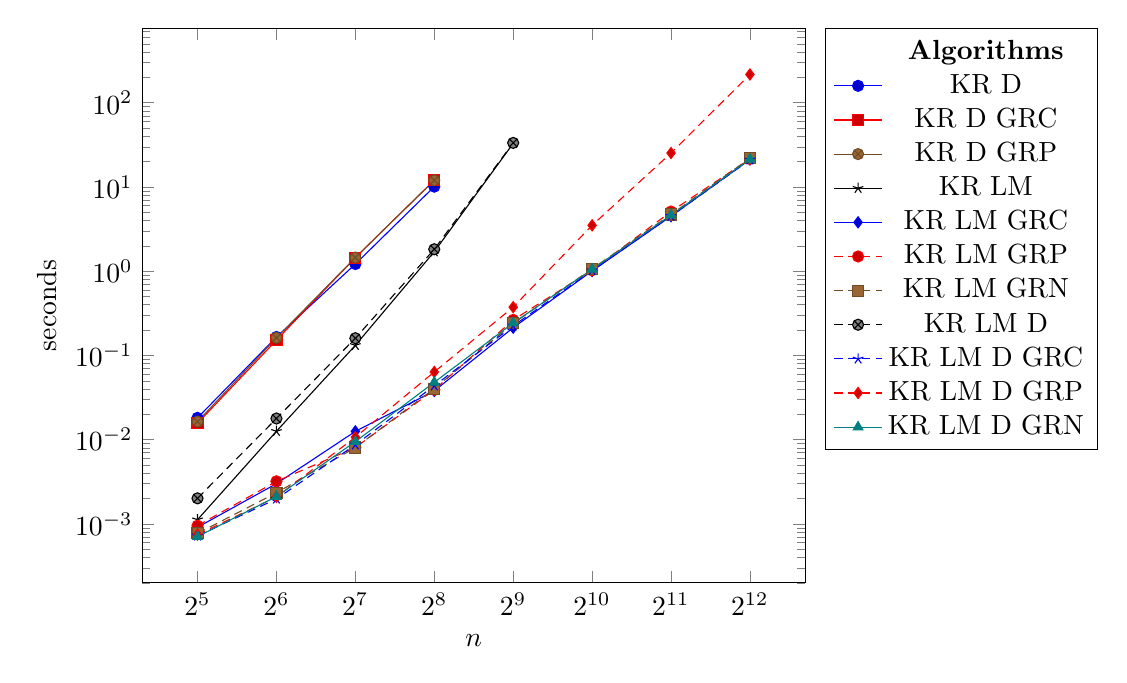
\begin{tikzpicture}
\begin{axis}[
    xlabel=$n$,ylabel=seconds,
    xmode=log,ymode=log,
    log basis x={2},
    legend style=
    {
        legend pos=outer north east
    },
    width=10cm
]
\addlegendimage{legend image code/.code=}
\legend{\textbf{Algorithms}, KR D, KR D GRC, KR D GRP, KR LM, KR LM GRC, KR LM GRP, KR LM GRN, KR LM D, KR LM D GRC, KR LM D GRP, KR LM D GRN}
\addplot table[x=n,y=value] {%KR
n value
32	0.0181733
64	0.165739667
128	1.21656
256	10.09223333
};
\addplot table[x=n,y=value] {%KR GRC
n value
32	0.0156879
64	0.151962
128	1.45053
256	12.0393
};
\addplot table[x=n,y=value] {%KR GRP
n value
32	0.016405833
64	0.162039667
128	1.45158
256	12.01736667
};
\addplot table[x=n,y=value] {%KR LM
n value
32	0.00112349
64	0.012595033
128	0.131954333
256	1.705006667
512	32.9077
};
\addplot table[x=n,y=value] {%KR LM GRC
n value
32	0.000912274
64	0.00300656
128	0.012558933
256	0.037942
512	0.213656667
1024	1.007368333
2048	4.502716667
4096	21.199
};
\addplot table[x=n,y=value] {%KR LM GRP
n value
32	0.00095436
64	0.003208227
128	0.00807021
256	0.0391309
512	0.264306667
1024	1.029762667
2048	5.10844
4096	21.54473333
};
\addplot table[x=n,y=value] {%KR LM GRN
n value
32	0.000772573
64	0.002344813
128	0.008068313
256	0.040385667
512	0.240289667
1024	1.069216667
2048	4.716753333
4096	21.92293333
};
\addplot table[x=n,y=value] {%KR LM D
n value
32	0.002014107
64	0.017856
128	0.16025
256	1.82407
512	33.37643333
};
\addplot table[x=n,y=value] {%KR LM D GRC
n value
32	0.000722157
64	0.001982017
128	0.00869863
256	0.043668633
512	0.224592667
1024	1.017951333
2048	4.51069
4096	21.01986667
};
\addplot table[x=n,y=value] {%KR LM D GRP
n value
32	0.000746587
64	0.002094287
128	0.010713517
256	0.063737267
512	0.374642667
1024	3.505513333
2048	25.29676667
4096	216.746
};
\addplot[mark=triangle*, teal] table[x=n,y=value] {%KR LM D GRN
n value
32	0.000707387
64	0.002113277
128	0.009478093
256	0.0480019
512	0.243291
1024	1.052536667
2048	4.632166667
4096	21.3589
};
\end{axis}
\end{tikzpicture}
\caption{King and Rao results from the CRH graphs}
\label{fig:CRH_KR_Results}
\end{figure}

%-----------------------------------------------------------------------------------------------------------
\clearpage


\subsection{Results from CRE graphs}
\begin{figure}[h]
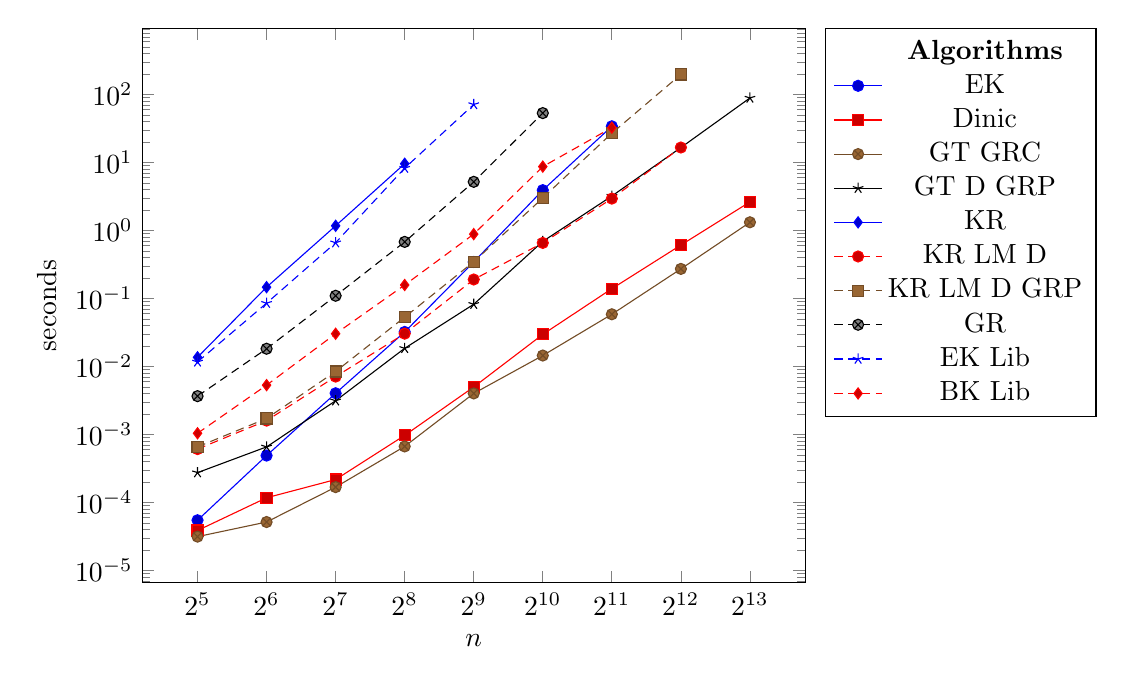
\begin{tikzpicture}
\begin{axis}[
    xlabel=$n$,ylabel=seconds,
    xmode=log,ymode=log,
    log basis x={2},
    legend style=
    {
        legend pos=outer north east
    },
    width=10cm
]
\addlegendimage{legend image code/.code=}
\legend{\textbf{Algorithms}, EK, Dinic, GT GRC, GT D GRP, KR, KR LM D, KR LM D GRP, GR, EK Lib, BK Lib}
\addplot table[x=n,y=value] {%EK
n value
32	5.47473E-05
64	0.000488839
128	0.00403531
256	0.032188067
512	0.344482667
1024	3.92213
2048	34.09136667
};
\addplot table[x=n,y=value] {%Dinic
n value
32	3.86452E-05
64	0.000117157
128	0.000217213
256	0.000969461
512	0.004991113
1024	0.0296234
2048	0.13921
4096	0.610286667
8192	2.630443333
};
\addplot table[x=n,y=value] {%GT GRC
n value
32	3.1427E-05
64	5.15269E-05
128	0.000168017
256	0.000666518
512	0.00401199
1024	0.0144843
2048	0.0585542
4096	0.272228333
8192	1.320586667
};
\addplot table[x=n,y=value] {%GT D GRP
n value
32	0.000274404
64	0.000656526
128	0.003130713
256	0.018493567
512	0.082231433
1024	0.691143667
2048	3.20825
4096	16.5731
8192	88.89143333
};
\addplot table[x=n,y=value] {%KR
n value
32	0.013644
64	0.146774
128	1.172116667
256	9.59715
};
\addplot table[x=n,y=value] {%KR LM D
n value
32	0.000609217
64	0.00159878
128	0.007093297
256	0.030375067
512	0.190262667
1024	0.656387333
2048	2.943613333
4096	16.61786667
};
\addplot table[x=n,y=value] {%KR LM D GRP
n value
32	0.000656525
64	0.001718273
128	0.008436667
256	0.0530621
512	0.346809
1024	3.012093333
2048	26.94046667
4096	197.305
};
\addplot table[x=n,y=value] {%GR
n value
32	0.003658853
64	0.0182312
128	0.109624667
256	0.679776333
512	5.196073333
1024	53.29516667
};
\addplot table[x=n,y=value] {%EK Lib
n value
32	0.011662833
64	0.0852518
128	0.661307667
256	8.265413333
512	71.3308
};
\addplot table[x=n,y=value] {%BK Lib
n value
32	0.001040203
64	0.005313077
128	0.030276133
256	0.157713
512	0.884518333
1024	8.698513333
2048	32.59023333
};
\end{axis}
\end{tikzpicture}
\caption{Best and worst results from the CRE graphs}
\label{fig:CRE_BW_Results}
\end{figure}


\begin{figure}[h]
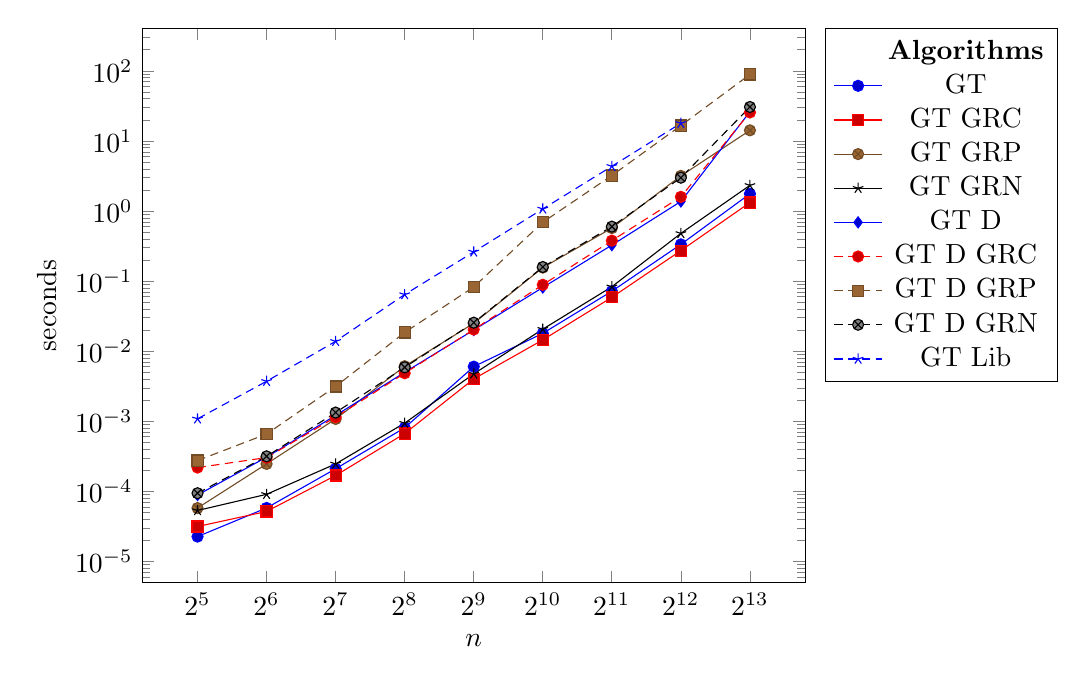
\begin{tikzpicture}
\begin{axis}[
    xlabel=$n$,ylabel=seconds,
    xmode=log,ymode=log,
    log basis x={2},
    legend style=
    {
        legend pos=outer north east
    },
    width=10cm
]
\addlegendimage{legend image code/.code=}
\legend{\textbf{Algorithms}, GT, GT GRC, GT GRP, GT GRN, GT D, GT D GRC, GT D GRP, GT D GRN, GT Lib}
\addplot table[x=n,y=value] {%GT
n value
32	0.000022543
64	5.78567E-05
128	0.000209439
256	0.000805885
512	0.006011103
1024	0.017948133
2048	0.071653367
4096	0.334158333
8192	1.76081
};
\addplot table[x=n,y=value] {%GT GRC
n value
32	3.1427E-05
64	5.15269E-05
128	0.000168017
256	0.000666518
512	0.00401199
1024	0.0144843
2048	0.0585542
4096	0.272228333
8192	1.320586667
};
\addplot table[x=n,y=value] {%GT GRP
n value
32	5.76346E-05
64	0.000245974
128	0.001076403
256	0.006092387
512	0.025003667
1024	0.155701
2048	0.570373667
4096	3.17186
8192	14.16263333
};
\addplot table[x=n,y=value] {%GT GRN
n value
32	5.31928E-05
64	9.05055E-05
128	0.000245975
256	0.000939036
512	0.004738823
1024	0.0205873
2048	0.082965767
4096	0.479294
8192	2.32381
};
\addplot table[x=n,y=value] {%GT D
n value
32	8.83956E-05
64	0.000307163
128	0.001209329
256	0.004990683
512	0.020028707
1024	0.081005167
2048	0.326051
4096	1.369142
8192	26.16655333
};
\addplot table[x=n,y=value] {%GT D GRC
n value
32	0.00021788
64	0.000302722
128	0.001143924
256	0.00483831
512	0.02032443
1024	0.088531933
2048	0.378064333
4096	1.592337667
8192	25.48298667
};
\addplot table[x=n,y=value] {%GT D GRP
n value
32	0.000274404
64	0.000656526
128	0.003130713
256	0.018493567
512	0.082231433
1024	0.691143667
2048	3.20825
4096	16.5731
8192	88.89143333
};
\addplot table[x=n,y=value] {%GT D GRN
n value
32	9.38368E-05
64	0.000315492
128	0.001328933
256	0.005874867
512	0.0254909
1024	0.158821667
2048	0.598509
4096	2.988956667
8192	30.53813333
};
\addplot table[x=n,y=value] {%GT Lib
n value
32	0.00108196
64	0.003715623
128	0.013819433
256	0.064229333
512	0.260638667
1024	1.070513333
2048	4.344643333
4096	17.865
};
\end{axis}
\end{tikzpicture}
\caption{Goldberg and Tarjan results from the CRE graphs}
\label{fig:CRE_GT_Results}
\end{figure}


\begin{figure}[h]
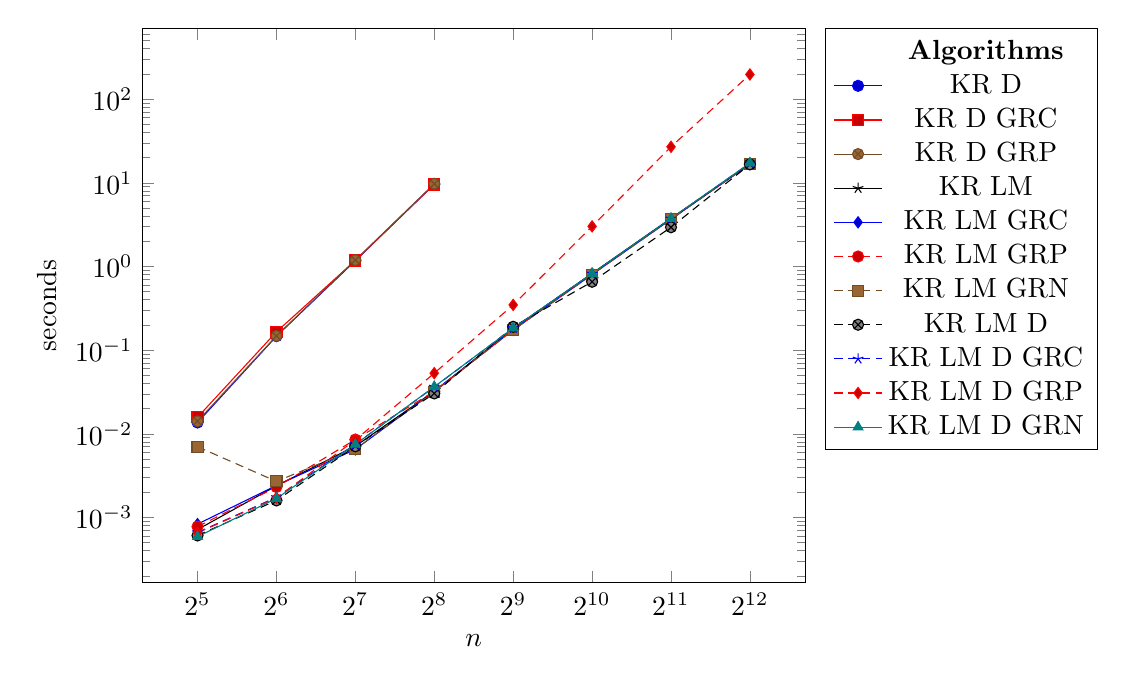
\begin{tikzpicture}
\begin{axis}[
    xlabel=$n$,ylabel=seconds,
    xmode=log,ymode=log,
    log basis x={2},
    legend style=
    {
        legend pos=outer north east
    },
    width=10cm
]
\addlegendimage{legend image code/.code=}
\legend{\textbf{Algorithms}, KR D, KR D GRC, KR D GRP, KR LM, KR LM GRC, KR LM GRP, KR LM GRN, KR LM D, KR LM D GRC, KR LM D GRP, KR LM D GRN}
\addplot table[x=n,y=value] {%KR
n value
32	0.013644
64	0.146774
128	1.172116667
256	9.59715
};
\addplot table[x=n,y=value] {%KR GRC
n value
32	0.015749367
64	0.165407333
128	1.180593333
256	9.566476667
};
\addplot table[x=n,y=value] {%KR GRP
n value
32	0.014125267
64	0.147867
128	1.192166667
256	9.735496667
};
\addplot table[x=n,y=value] {%KR LM
n value
32	0.000716493
64	0.002392677
128	0.007121063
256	0.0321503
512	0.180944667
1024	0.826992
2048	3.762636667
4096	16.7083
};
\addplot table[x=n,y=value] {%KR LM GRC
n value
32	0.00083254
64	0.002410663
128	0.006525943
256	0.032414067
512	0.174600667
1024	0.801770333
2048	3.67155
4096	16.72523333
};
\addplot table[x=n,y=value] {%KR LM GRP
n value
32	0.000777125
64	0.0023105
128	0.008542273
256	0.0321469
512	0.175911
1024	0.808778333
2048	3.688806667
4096	16.86536667
};
\addplot table[x=n,y=value] {%KR LM GRN
n value
32	0.007005796
64	0.002697727
128	0.006570027
256	0.031863467
512	0.173352333
1024	0.798951667
2048	3.65546
4096	16.72086667
};
\addplot table[x=n,y=value] {%KR LM D
n value
32	0.000609217
64	0.00159878
128	0.007093297
256	0.030375067
512	0.190262667
1024	0.656387333
2048	2.943613333
4096	16.61786667
};
\addplot table[x=n,y=value] {%KR LM D GRC
n value
32	0.00066219
64	0.001740923
128	0.007506513
256	0.0362996
512	0.183215667
1024	0.817935
2048	3.727963333
4096	17.15916667
};
\addplot table[x=n,y=value] {%KR LM D GRP
n value
32	0.000656525
64	0.001718273
128	0.008436667
256	0.0530621
512	0.346809
1024	3.012093333
2048	26.94046667
4096	197.305
};
\addplot[mark=triangle*, teal] table[x=n,y=value] {%KR LM D GRN
n value
32	0.000590452
64	0.00168551
128	0.00747431
256	0.036542667
512	0.183141
1024	0.823798
2048	3.743673333
4096	17.22786667
};
\end{axis}
\end{tikzpicture}
\caption{King and Rao results from the CRE graphs}
\label{fig:CRE_KR_Results}
\end{figure}

%-----------------------------------------------------------------------------------------------------------

\clearpage

\subsection{Results from CD graphs}
\begin{figure}[h]
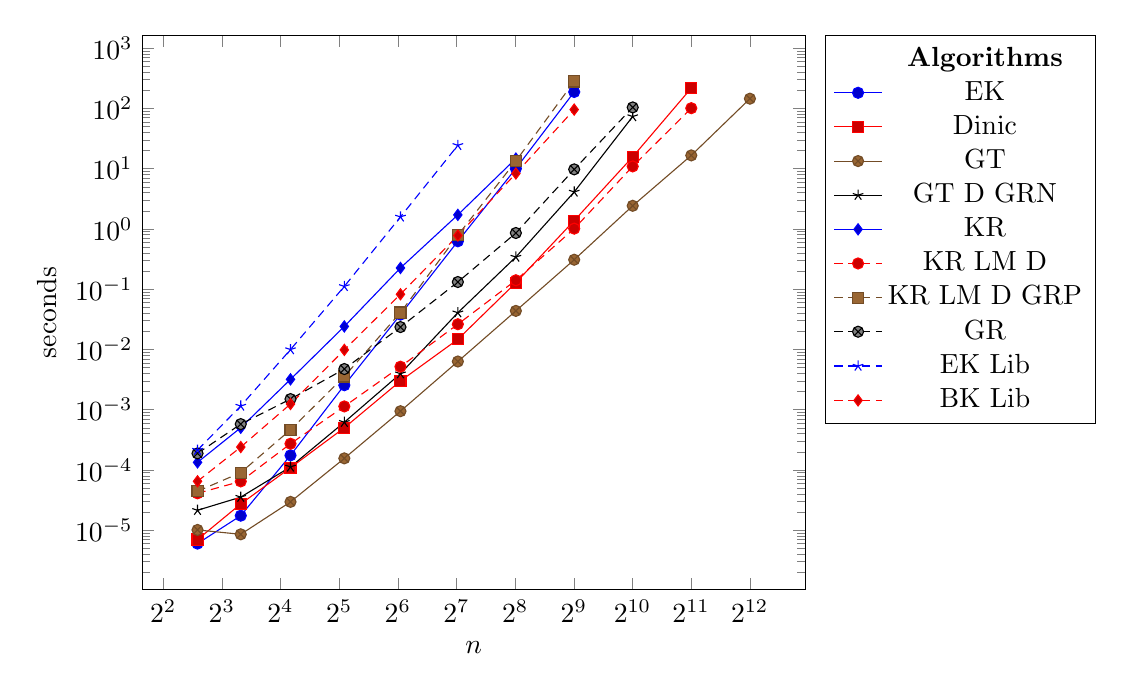
\begin{tikzpicture}
\begin{axis}[
    xlabel=$n$,ylabel=seconds,
    xmode=log,ymode=log,
    log basis x={2},
    legend style=
    {
        legend pos=outer north east
    },
    width=10cm
]
\addlegendimage{legend image code/.code=}
\legend{\textbf{Algorithms}, EK, Dinic, GT, GT D GRN, KR, KR LM D, KR LM D GRP, GR, EK Lib, BK Lib}
\addplot table[x=n,y=value] {%EK
n value
6	5.99667E-06
10	1.74347E-05
18	0.000174792
34	0.002550027
66	0.037885933
130	0.624042667
258	10.04213333
514	187.6203333
};
\addplot table[x=n,y=value] {%Dinic
n value
6	6.99611E-06
10	2.73181E-05
18	0.00010905
34	0.000501499
66	0.00300133
130	0.0147208
258	0.128177333
514	1.37476
1026	15.72296667
2050	217.4116667
};
\addplot table[x=n,y=value] {%GT
n value
6	1.01055E-05
10	8.5508E-06
18	2.95391E-05
34	0.000155802
66	0.000944475
130	0.006306823
258	0.043635633
514	0.308285667
1026	2.421146667
2050	16.61676667
4098	145.0676667
};
\addplot table[x=n,y=value] {%GT D GRN
n value
6	2.14326E-05
10	3.54248E-05
18	0.000112493
34	0.00061999
66	0.003963697
130	0.040730567
258	0.341904333
514	4.108336667
1026	73.36176667
};
\addplot table[x=n,y=value] {%KR
n value
6	0.000133704
10	0.000502276
18	0.00318767
34	0.0240945
66	0.225141333
130	1.711946667
258	14.71456667
};
\addplot table[x=n,y=value] {%KR LM D
n value
6	4.09773E-05
10	6.46309E-05
18	0.000272405
34	0.00113404
66	0.00517125
130	0.0262096
258	0.140639
514	1.011333333
1026	10.91203333
2050	100.9013333
};
\addplot table[x=n,y=value] {%KR LM D GRP
n value
6	4.43088E-05
10	9.02832E-05
18	0.000464965
34	0.003558917
66	0.040930333
130	0.784254333
258	13.388
514	280.4783333
};
\addplot table[x=n,y=value] {%GR
n value
6	0.000188451
10	0.000577012
18	0.001500943
34	0.004733923
66	0.023517667
130	0.131538667
258	0.856225667
514	9.73903
1026	103.9606667
};
\addplot table[x=n,y=value] {%EK Lib
n value
6	0.000213883
10	0.00115181
18	0.009964183
34	0.111426
66	1.58397
130	24.43106667
};
\addplot table[x=n,y=value] {%BK Lib
n value
6	6.48532E-05
10	0.000239979
18	0.001242873
34	0.00983991
66	0.082395133
130	0.777942
258	8.31923
514	95.6544
};
\end{axis}
\end{tikzpicture}
\caption{Best and worst results from the CD graphs}
\label{fig:CD_BW_Results}
\end{figure}


\begin{figure}[h]
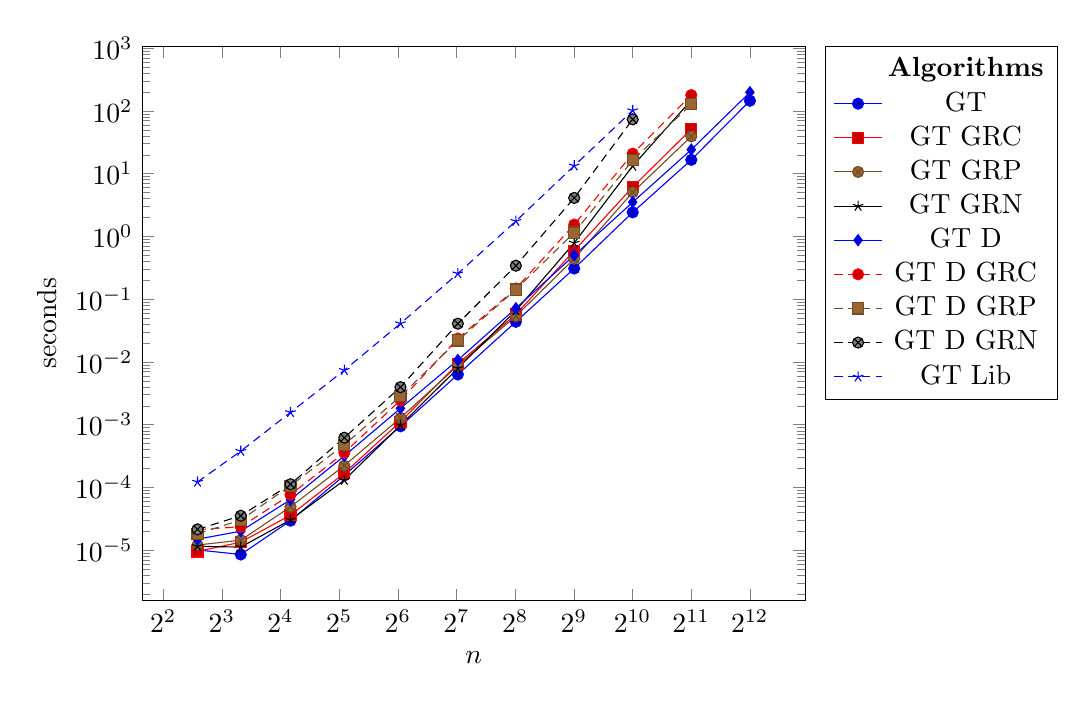
\begin{tikzpicture}
\begin{axis}[
    xlabel=$n$,ylabel=seconds,
    xmode=log,ymode=log,
    log basis x={2},
    legend style=
    {
        legend pos=outer north east
    },
    width=10cm
]
\addlegendimage{legend image code/.code=}
\legend{\textbf{Algorithms}, GT, GT GRC, GT GRP, GT GRN, GT D, GT D GRC, GT D GRP, GT D GRN, GT Lib}
\addplot table[x=n,y=value] {%GT
n value
6	1.01055E-05
10	8.5508E-06
18	2.95391E-05
34	0.000155802
66	0.000944475
130	0.006306823
258	0.043635633
514	0.308285667
1026	2.421146667
2050	16.61676667
4098	145.0676667
};
\addplot table[x=n,y=value] {%GT GRC
n value
6	9.55024E-06
10	1.34369E-05
18	3.62021E-05
34	0.000169017
66	0.001118267
130	0.009349797
258	0.057142333
514	0.591681667
1026	6.116086667
2050	51.259
};
\addplot table[x=n,y=value] {%GT GRP
n value
6	1.21044E-05
10	1.44364E-05
18	4.91949E-05
34	0.000222876
66	0.00128251
130	0.008756907
258	0.053604167
514	0.441572333
1026	5.047726667
2050	39.2892
};
\addplot table[x=n,y=value] {%GT GRN
n value
6	1.15492E-05
10	1.1216E-05
18	3.04276E-05
34	0.000130594
66	0.000979679
130	0.007932053
258	0.0657545
514	0.788411667
1026	13.26623333
2050	148.4456667
};
\addplot table[x=n,y=value] {%GT D
n value
6	1.49917E-05
10	2.01E-05
18	6.38536E-05
34	0.000318379
66	0.00181977
130	0.010725967
258	0.071542
514	0.499891
1026	3.513503333
2050	24.14273333
4098	198.0083333
};
\addplot table[x=n,y=value] {%GT D GRC
n value
6	2.13216E-05
10	2.36536E-05
18	7.66243E-05
34	0.000357802
66	0.00245109
130	0.023582033
258	0.147942
514	1.545093333
1026	20.85666667
2050	178.8586667
};
\addplot table[x=n,y=value] {%GT D GRP
n value
6	1.82122E-05
10	3.03165E-05
18	0.000106608
34	0.000480068
66	0.002840317
130	0.021989267
258	0.142533333
514	1.151853333
1026	16.32986667
2050	127.8266667
};
\addplot table[x=n,y=value] {%GT D GRN
n value
6	2.14326E-05
10	3.54248E-05
18	0.000112493
34	0.00061999
66	0.003963697
130	0.040730567
258	0.341904333
514	4.108336667
1026	73.36176667
};
\addplot table[x=n,y=value] {%GT Lib
n value
6	0.000122266
10	0.000379236
18	0.001570913
34	0.007375277
66	0.040921467
130	0.25571
258	1.75135
514	13.36043333
1026	101.6196667
};
\end{axis}
\end{tikzpicture}
\caption{Goldberg and Tarjan results from the CD graphs}
\label{fig:CD_GT_Results}
\end{figure}


\begin{figure}[h]
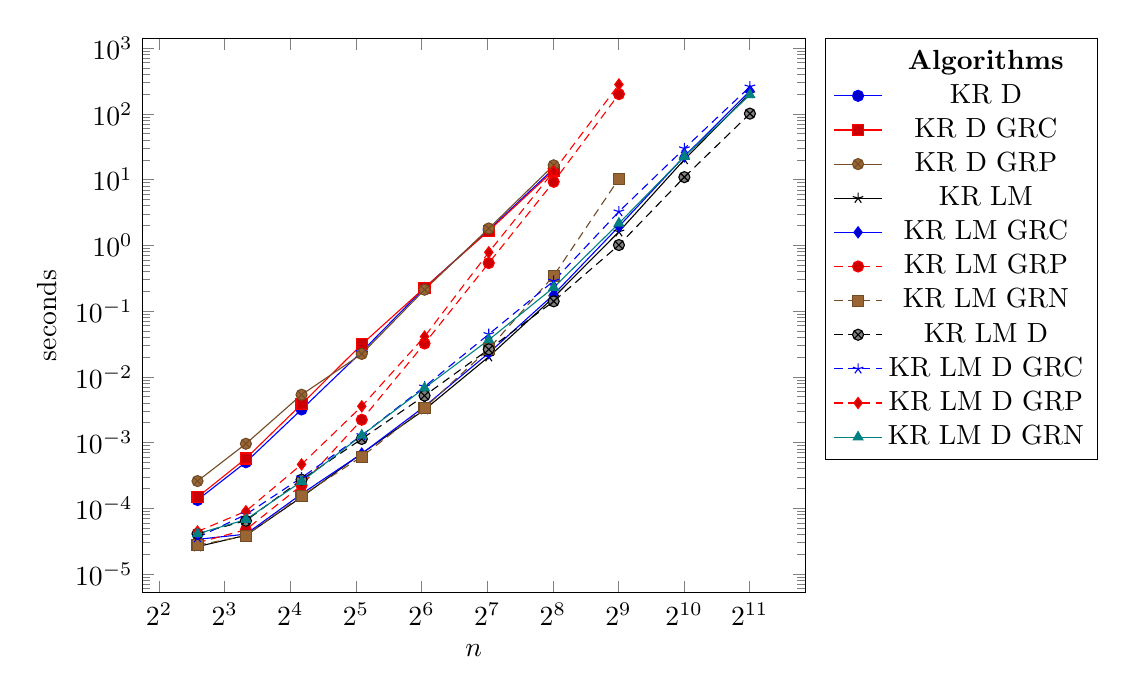
\begin{tikzpicture}
\begin{axis}[
    xlabel=$n$,ylabel=seconds,
    xmode=log,ymode=log,
    log basis x={2},
    legend style=
    {
        legend pos=outer north east
    },
    width=10cm
]
\addlegendimage{legend image code/.code=}
\legend{\textbf{Algorithms}, KR D, KR D GRC, KR D GRP, KR LM, KR LM GRC, KR LM GRP, KR LM GRN, KR LM D, KR LM D GRC, KR LM D GRP, KR LM D GRN}
\addplot table[x=n,y=value] {%KR
n value
6	0.000133704
10	0.000502276
18	0.00318767
34	0.0240945
66	0.225141333
130	1.711946667
258	14.71456667
};
\addplot table[x=n,y=value] {%KR GRC
n value
6	0.000147696
10	0.000572126
18	0.00383287
34	0.031165867
66	0.226962667
130	1.665713333
258	13.78036667
};
\addplot table[x=n,y=value] {%KR GRP
n value
6	0.00025919
10	0.000958247
18	0.005336383
34	0.022293567
66	0.211193
130	1.80843
258	16.52083333
};
\addplot table[x=n,y=value] {%KR LM
n value
6	2.60967E-05
10	3.87563E-05
18	0.00014814
34	0.000683844
66	0.00316436
130	0.020178967
258	0.161748
514	1.60653
1026	20.2325
2050	204.3513333
};
\addplot table[x=n,y=value] {%KR LM GRC
n value
6	3.36481E-05
10	4.04221E-05
18	0.000165353
34	0.000677847
66	0.00354215
130	0.022967967
258	0.178342667
514	1.937253333
1026	22.58583333
2050	222.2673333
};
\addplot table[x=n,y=value] {%KR LM GRP
n value
6	2.98723E-05
10	4.71961E-05
18	0.000222988
34	0.002223993
66	0.032125767
130	0.537739667
258	9.257863333
514	199.7963333
};
\addplot table[x=n,y=value] {%KR LM GRN
n value
6	2.74293E-05
10	3.82011E-05
18	0.000154914
34	0.000610884
66	0.003374687
130	0.0266112
258	0.343906
514	10.29113333
};
\addplot table[x=n,y=value] {%KR LM D
n value
6	4.09773E-05
10	6.46309E-05
18	0.000272405
34	0.00113404
66	0.00517125
130	0.0262096
258	0.140639
514	1.011333333
1026	10.91203333
2050	100.9013333
};
\addplot table[x=n,y=value] {%KR LM D GRC
n value
6	3.58691E-05
10	8.03999E-05
18	0.000291727
34	0.00128762
66	0.007077527
130	0.044424067
258	0.286881
514	3.257403333
1026	29.71603333
2050	258.9453333
};
\addplot table[x=n,y=value] {%KR LM D GRP
n value
6	4.43088E-05
10	9.02832E-05
18	0.000464965
34	0.003558917
66	0.040930333
130	0.784254333
258	13.388
514	280.4783333
};
\addplot[mark=triangle*, teal] table[x=n,y=value] {%KR LM D GRN
n value
6	4.09774E-05
10	6.72961E-05
18	0.000255414
34	0.001285843
66	0.00676959
130	0.0364898
258	0.228359667
514	2.162886667
1026	22.46466667
2050	194.565
};
\end{axis}
\end{tikzpicture}
\caption{King and Rao results from the CD graphs}
\label{fig:CD_KR_Results}
\end{figure}

%-----------------------------------------------------------------------------------------------------------
\clearpage


\subsection{Results from AK graphs}
\begin{figure}[h]
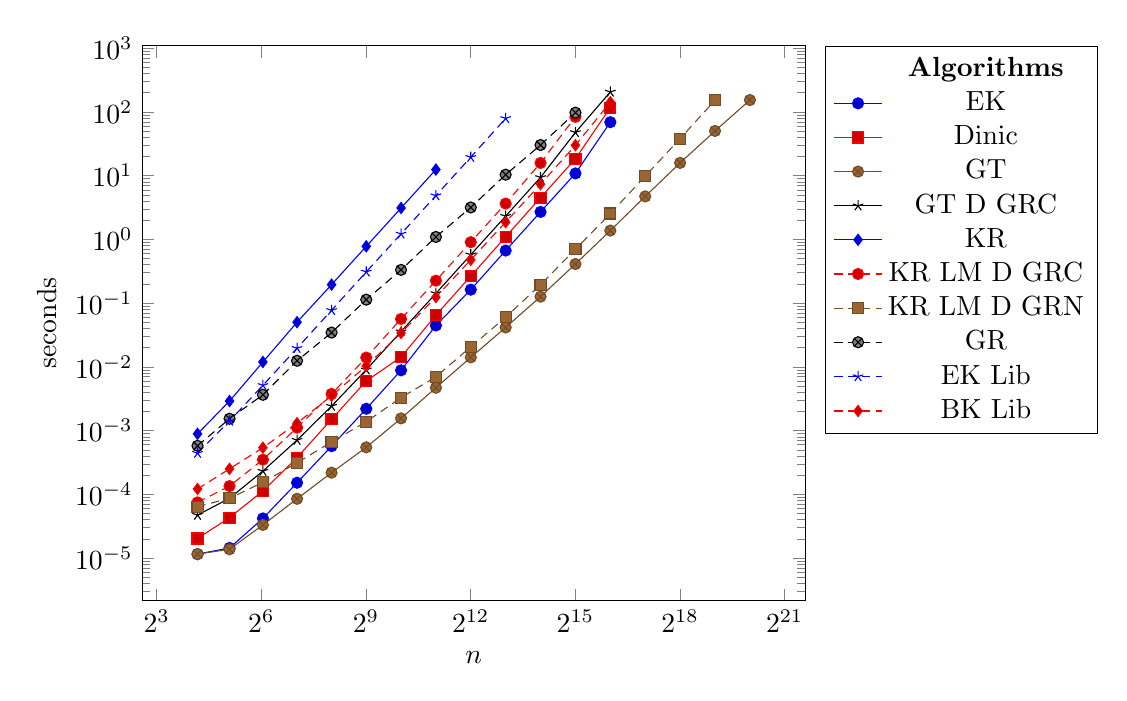
\begin{tikzpicture}
\begin{axis}[
    xlabel=$n$,ylabel=seconds,
    xmode=log,ymode=log,
    log basis x={2},
    legend style=
    {
        legend pos=outer north east
    },
    width=10cm
]
\addlegendimage{legend image code/.code=}
\legend{\textbf{Algorithms}, EK, Dinic, GT, GT D GRC, KR, KR LM D GRC, KR LM D GRN, GR, EK Lib, BK Lib}
\addplot table[x=n,y=value] {%EK
n value
18	1.15491E-05
34	1.44364E-05
66	4.19766E-05
130	0.000152249
258	0.000570682
514	0.002202887
1026	0.008838197
2050	0.0446577
4098	0.162670667
8194	0.668331333
16386	2.69851
32770	10.8331
65538	69.00813333
};
\addplot table[x=n,y=value] {%Dinic
n value
18	2.0322E-05
34	4.30871E-05
66	0.000113381
130	0.000376457
258	0.001508607
514	0.00600899
1026	0.014264533
2050	0.064598533
4098	0.265333667
8194	1.096893333
16386	4.517406667
32770	18.42716667
65538	116.604
};
\addplot table[x=n,y=value] {%GT
n value
18	1.15491E-05
34	1.37701E-05
66	3.32038E-05
130	8.51749E-05
258	0.000218989
514	0.000547029
1026	0.001555913
2050	0.004708267
4098	0.014102167
8194	0.041543667
16386	0.126403
32770	0.410714667
65538	1.375183333
131074	4.7243
262146	15.85233333
524290	50.24406667
1048578	153.437
};
\addplot table[x=n,y=value] {%GT D GRC
n value
18	4.73071E-05
34	8.68408E-05
66	0.000231983
130	0.000709607
258	0.002425103
514	0.009009903
1026	0.0358142
2050	0.142085333
4098	0.575261667
8194	2.315736667
16386	9.388776667
32770	47.68883333
65538	205.5886667
};
\addplot table[x=n,y=value] {%KR
n value
18	0.000889175
34	0.002908057
66	0.011943033
130	0.050249867
258	0.195147333
514	0.777756
1026	3.107726667
2050	12.4823
};
\addplot table[x=n,y=value] {%KR LM D GRC
n value
18	7.48474E-05
34	0.000134814
66	0.000350584
130	0.00111305
258	0.003765693
514	0.014000933
1026	0.0564863
2050	0.225324667
4098	0.904017333
8194	3.646476667
16386	15.8397
32770	83.65686667
};
\addplot table[x=n,y=value] {%KR LM D GRN
n value
18	6.41867E-05
34	8.66187E-05
66	0.00015447
130	0.000312605
258	0.000664521
514	0.001379017
1026	0.003295733
2050	0.006980693
4098	0.020601467
8194	0.0600087
16386	0.194730333
32770	0.69788
65538	2.548136667
131074	9.800743333
262146	38.14566667
524290	152.5736667
};
\addplot table[x=n,y=value] {%GR
n value
18	0.000578012
34	0.001536363
66	0.003647417
130	0.012470067
258	0.034521233
514	0.113386
1026	0.332325333
2050	1.092523333
4098	3.170253333
8194	10.35553333
16386	30.2229
32770	97.3555
};
\addplot table[x=n,y=value] {%EK Lib
n value
18	0.000443645
34	0.001415443
66	0.005145503
130	0.019632167
258	0.077202333
514	0.309274333
1026	1.21978
2050	4.860823333
4098	19.46263333
8194	79.22313333
};
\addplot table[x=n,y=value] {%BK Lib
n value
18	0.000121378
34	0.000251306
66	0.000539481
130	0.001310057
258	0.003520287
514	0.010349767
1026	0.0339719
2050	0.124275
4098	0.477602
8194	1.861176667
16386	7.34532
32770	29.98583333
65538	142.366
};
\end{axis}
\end{tikzpicture}
\caption{Best and worst results from the AK graphs}
\label{fig:AK_BW_Results}
\end{figure}


\begin{figure}[h]
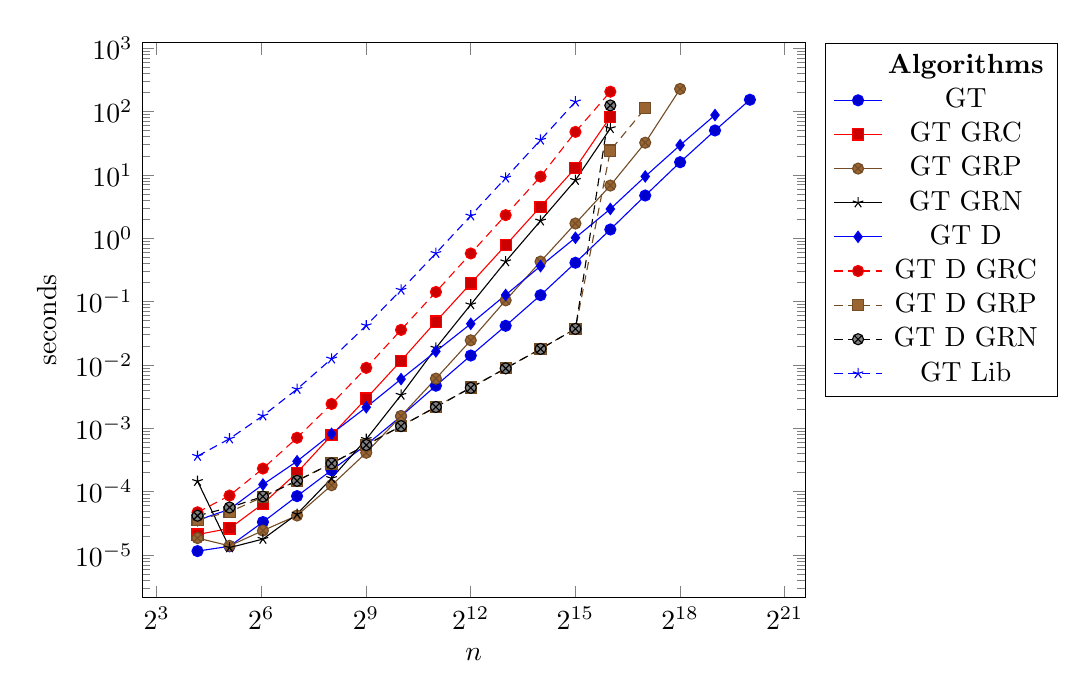
\begin{tikzpicture}
\begin{axis}[
    xlabel=$n$,ylabel=seconds,
    xmode=log,ymode=log,
    log basis x={2},
    legend style=
    {
        legend pos=outer north east
    },
    width=10cm
]
\addlegendimage{legend image code/.code=}
\legend{\textbf{Algorithms}, GT, GT GRC, GT GRP, GT GRN, GT D, GT D GRC, GT D GRP, GT D GRN, GT Lib}
\addplot table[x=n,y=value] {%GT
n value
18	1.15491E-05
34	1.37701E-05
66	3.32038E-05
130	8.51749E-05
258	0.000218989
514	0.000547029
1026	0.001555913
2050	0.004708267
4098	0.014102167
8194	0.041543667
16386	0.126403
32770	0.410714667
65538	1.375183333
131074	4.7243
262146	15.85233333
524290	50.24406667
1048578	153.437
};
\addplot table[x=n,y=value] {%GT GRC
n value
18	2.10994E-05
34	2.63187E-05
66	6.45197E-05
130	0.000200222
258	0.000779344
514	0.002955247
1026	0.011688167
2050	0.0483993
4098	0.193606
8194	0.774928333
16386	3.153233333
32770	12.85786667
65538	82.32676667
};
\addplot table[x=n,y=value] {%GT GRP
n value
18	1.85453E-05
34	1.39922E-05
66	2.43198E-05
130	4.20877E-05
258	0.000126596
514	0.000411993
1026	0.001565127
2050	0.006093057
4098	0.0244856
8194	0.104717
16386	0.428277667
32770	1.70907
65538	6.788133333
131074	32.18266667
262146	227.165
};
\addplot table[x=n,y=value] {%GT GRN
n value
18	0.000146252
34	1.31039E-05
66	0.000017879
130	4.43088E-05
258	0.00016291
514	0.000673739
1026	0.003355143
2050	0.018532733
4098	0.089804633
8194	0.429052667
16386	1.885126667
32770	8.247653333
65538	54.24016667
};
\addplot table[x=n,y=value] {%GT D
n value
18	3.54249E-05
34	5.28596E-05
66	0.000129928
130	0.00030261
258	0.000819102
514	0.002152143
1026	0.005989243
2050	0.016409467
4098	0.044628533
8194	0.127470333
16386	0.363211
32770	1.019396667
65538	2.897966667
131074	9.462753333
262146	29.41903333
524290	88.0256
};
\addplot table[x=n,y=value] {%GT D GRC
n value
18	4.73071E-05
34	8.68408E-05
66	0.000231983
130	0.000709607
258	0.002425103
514	0.009009903
1026	0.0358142
2050	0.142085333
4098	0.575261667
8194	2.315736667
16386	9.388776667
32770	47.68883333
65538	205.5886667
};
\addplot table[x=n,y=value] {%GT D GRP
n value
18	3.60912E-05
34	4.79734E-05
66	8.2621E-05
130	0.000149362
258	0.000279179
514	0.000546364
1026	0.00109295
2050	0.002178017
4098	0.00441367
8194	0.008896857
16386	0.017891767
32770	0.0374025
65538	24.21606667
131074	112.5863333
};
\addplot table[x=n,y=value] {%GT D GRN
n value
18	4.17547E-05
34	5.64132E-05
66	8.40646E-05
130	0.000148473
258	0.000279623
514	0.000545365
1026	0.001084287
2050	0.002170243
4098	0.00436003
8194	0.008836443
16386	0.0179194
32770	0.037174767
65538	124.819
};
\addplot table[x=n,y=value] {%GT Lib
n value
18	0.000364577
34	0.000685067
66	0.001577687
130	0.00415938
258	0.012518467
514	0.0419147
1026	0.152552
2050	0.579812333
4098	2.263826667
8194	8.971396667
16386	35.5501
32770	142.772
};
\end{axis}
\end{tikzpicture}
\caption{Goldberg and Tarjan results from the AK graphs}
\label{fig:AK_GT_ResultsAppendix}
\end{figure}


\begin{figure}[h]
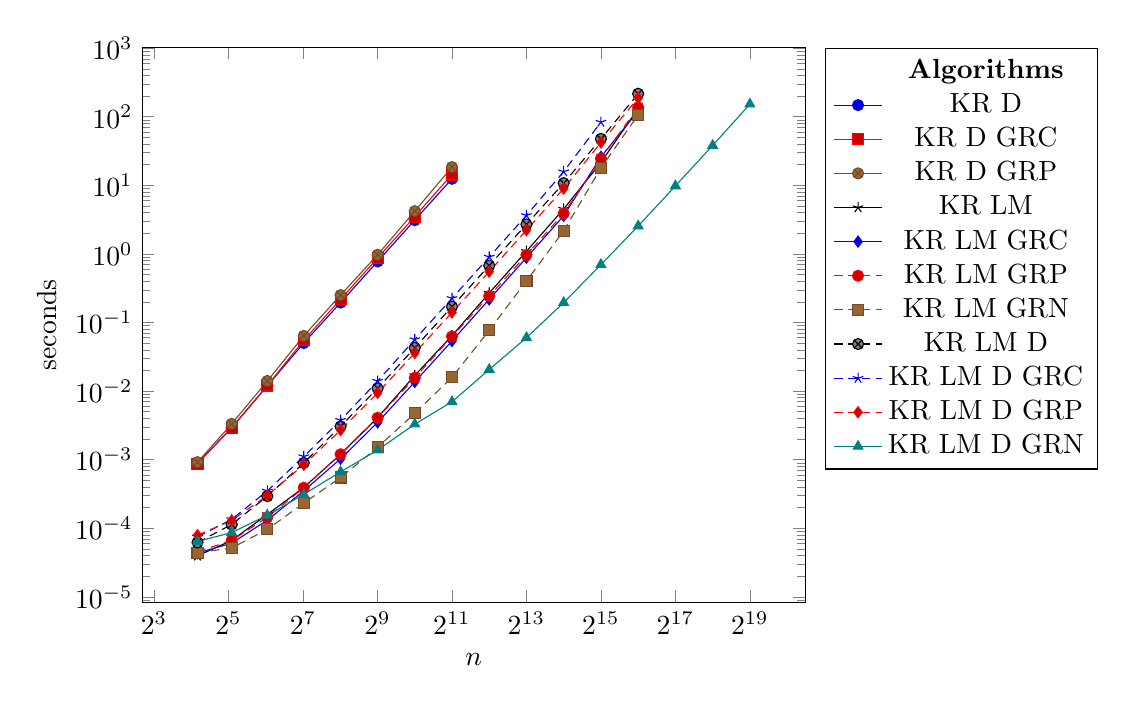
\begin{tikzpicture}
\begin{axis}[
    xlabel=$n$,ylabel=seconds,
    xmode=log,ymode=log,
    log basis x={2},
    legend style=
    {
        legend pos=outer north east
    },
    width=10cm
]
\addlegendimage{legend image code/.code=}
\legend{\textbf{Algorithms}, KR D, KR D GRC, KR D GRP, KR LM, KR LM GRC, KR LM GRP, KR LM GRN, KR LM D, KR LM D GRC, KR LM D GRP, KR LM D GRN}
\addplot table[x=n,y=value] {%KR
n value
18	0.000889175
34	0.002908057
66	0.011943033
130	0.050249867
258	0.195147333
514	0.777756
1026	3.107726667
2050	12.4823
};
\addplot table[x=n,y=value] {%KR GRC
n value
18	0.000875735
34	0.002938147
66	0.0120653
130	0.054935867
258	0.218274
514	0.872710333
1026	3.5095
2050	14.403
};
\addplot table[x=n,y=value] {%KR GRP
n value
18	0.000919492
34	0.00332838
66	0.014040333
130	0.0638248
258	0.251151333
514	0.971965333
1026	4.19931
2050	18.4658
};
\addplot table[x=n,y=value] {%KR LM
n value
18	3.95337E-05
34	6.66298E-05
66	0.000158912
130	0.000393449
258	0.00119856
514	0.00412505
1026	0.016918733
2050	0.064206667
4098	0.268975333
8194	1.09322
16386	4.51368
32770	21.53186667
65538	131.6553333
};
\addplot table[x=n,y=value] {%KR LM GRC
n value
18	4.34204E-05
34	6.07442E-05
66	0.000131261
130	0.000351139
258	0.001029877
514	0.00350173
1026	0.013609367
2050	0.0537659
4098	0.217405
8194	0.881691
16386	3.602213333
32770	26.04033333
65538	120.6886667
};
\addplot table[x=n,y=value] {%KR LM GRP
n value
18	4.57524E-05
34	6.62967E-05
66	0.000144697
130	0.000389451
258	0.00119834
514	0.00407752
1026	0.015643533
2050	0.062576267
4098	0.243189667
8194	0.966999333
16386	3.8901
32770	24.61043333
65538	136.8136667
};
\addplot table[x=n,y=value] {%KR LM GRN
n value
18	4.38646E-05
34	5.16381E-05
66	9.65021E-05
130	0.000232649
258	0.000549696
514	0.00151394
1026	0.00474304
2050	0.0158961
4098	0.0767171
8194	0.402905667
16386	2.16554
32770	17.93576667
65538	106.1156667
};
\addplot table[x=n,y=value] {%KR LM D
n value
18	6.21878E-05
34	0.000113493
66	0.000293837
130	0.000895949
258	0.003054753
514	0.010999333
1026	0.0427871
2050	0.170356
4098	0.676120333
8194	2.693893333
16386	10.74853333
32770	47.54073333
65538	216.514
};
\addplot table[x=n,y=value] {%KR LM D GRC
n value
18	7.48474E-05
34	0.000134814
66	0.000350584
130	0.00111305
258	0.003765693
514	0.014000933
1026	0.0564863
2050	0.225324667
4098	0.904017333
8194	3.646476667
16386	15.8397
32770	83.65686667
};
\addplot table[x=n,y=value] {%KR LM D GRP
n value
18	7.94004E-05
34	0.000130039
66	0.000300056
130	0.000844977
258	0.002696287
514	0.009420677
1026	0.035984667
2050	0.140029
4098	0.551803333
8194	2.21699
16386	8.955463333
32770	42.12056667
65538	186.7876667
};
\addplot[mark=triangle*, teal] table[x=n,y=value] {%KR LM D GRN
n value
18	6.41867E-05
34	8.66187E-05
66	0.00015447
130	0.000312605
258	0.000664521
514	0.001379017
1026	0.003295733
2050	0.006980693
4098	0.020601467
8194	0.0600087
16386	0.194730333
32770	0.69788
65538	2.548136667
131074	9.800743333
262146	38.14566667
524290	152.5736667
};
\end{axis}
\end{tikzpicture}
\caption{King and Rao results from the AK graphs}
\label{fig:AK_KR_ResultsAppendix}
\end{figure}

%-----------------------------------------------------------------------------------------------------------
\clearpage


\subsection{Results from GenRmf long graphs}
\begin{figure}[h]
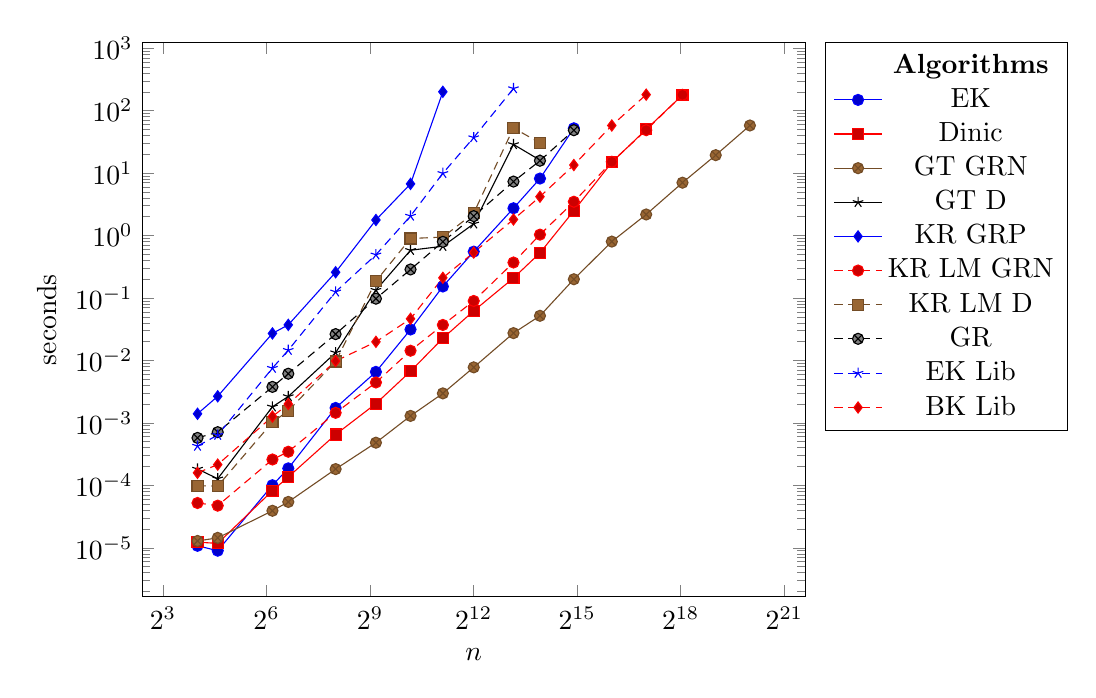
\begin{tikzpicture}
\begin{axis}[
    xlabel=$n$,ylabel=seconds,
    xmode=log,ymode=log,
    log basis x={2},
    legend style=
    {
        legend pos=outer north east
    },
    width=10cm
]
\addlegendimage{legend image code/.code=}
\legend{\textbf{Algorithms}, EK, Dinic, GT GRN, GT D, KR GRP, KR LM GRN, KR LM D, GR, EK Lib, BK Lib}
\addplot table[x=n,y=value] {%EK
n value
16	1.07718E-05
24	8.99499E-06
72	0.0001005
99	0.000187118
256	0.001736033
575	0.006561127
1152	0.031316167
2205	0.152855333
4096	0.552244333
9100	2.735133333
15488	8.1725
30589	52.13166667
};
\addplot table[x=n,y=value] {%Dinic
n value
16	1.23265E-05
24	1.17712E-05
72	8.21765E-05
99	0.000136146
256	0.000651637
575	0.002034203
1152	0.006705713
2205	0.022681033
4096	0.0621048
9100	0.208537333
15488	0.527127667
30589	2.491446667
65536	14.86433333
130682	50.06016667
270848	177.8626667
};
\addplot table[x=n,y=value] {%GT GRN
n value
16	1.28818E-05
24	1.44365E-05
72	3.92005E-05
99	5.43033E-05
256	0.000182232
575	0.000482289
1152	0.001294393
2205	0.002970023
4096	0.00775149
9100	0.0273884
15488	0.051847533
30589	0.199656667
65536	0.799864667
130682	2.173773333
270848	7.017736667
527796	19.36696667
1048576	57.80963333
};
\addplot table[x=n,y=value] {%GT D
n value
16	0.000182899
24	0.000127707
72	0.001811667
99	0.002649647
256	0.01333294
575	0.133493
1152	0.581190667
2205	0.673778667
4096	1.540246667
9100	28.75023333
15488	16.11123333
};
\addplot table[x=n,y=value] {%KR GRP
n value
16	0.00139845
24	0.002666637
72	0.0271098
99	0.037121367
256	0.258182333
575	1.773686667
1152	6.72207
2205	200.141
};
\addplot table[x=n,y=value] {%KR LM GRN
n value
16	5.21933E-05
24	4.73072E-05
72	0.000259523
99	0.000345365
256	0.001449643
575	0.00443921
1152	0.014312
2205	0.037018833
4096	0.089594333
9100	0.369817
15488	1.033306667
30589	3.473556667
65536	15.1593
130682	48.64013333
270848	178.9876667
};
\addplot table[x=n,y=value] {%KR LM D
n value
16	9.88343E-05
24	9.73907E-05
72	0.001024097
99	0.001562027
256	0.009612567
575	0.186065333
1152	0.896549
2205	0.943830667
4096	2.28156
9100	52.7981
15488	30.36093333
};
\addplot table[x=n,y=value] {%GR
n value
16	0.000575236
24	0.000710605
72	0.003772567
99	0.00613292
256	0.026391333
575	0.097505533
1152	0.286460667
2205	0.792706667
4096	2.04237
9100	7.310506667
15488	15.76233333
30589	48.56896667
};
\addplot table[x=n,y=value] {%EK Lib
n value
16	0.000425988
24	0.000638093
72	0.007533857
99	0.014606733
256	0.125504667
575	0.491983667
1152	2.055623333
2205	9.923236667
4096	37.06083333
9100	225.8106667
};
\addplot table[x=n,y=value] {%BK Lib
n value
16	0.00015869
24	0.000214993
72	0.00126475
99	0.002003343
256	0.009785063
575	0.019859533
1152	0.0464782
2205	0.210524
4096	0.53478
9100	1.80975
15488	4.18626
30589	13.45136667
65536	57.83356667
130682	180.1683333
};
\end{axis}
\end{tikzpicture}
\caption{Best and worst results from the GenRmf long graphs}
\label{fig:GenRmf long_BW_Results}
\end{figure}


\begin{figure}[h]
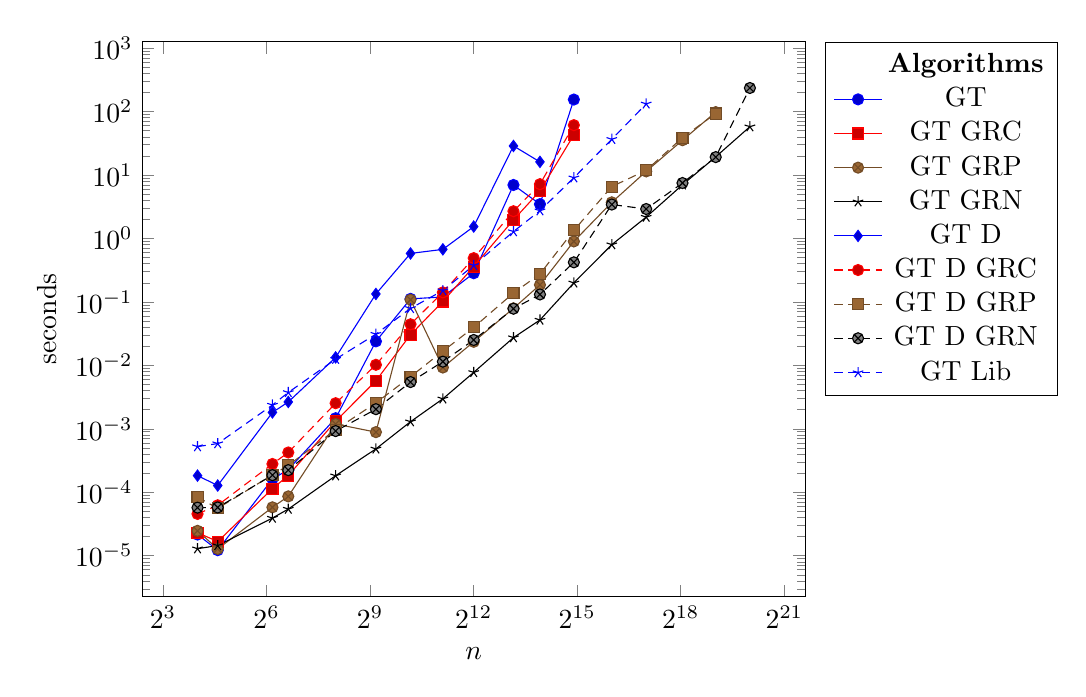
\begin{tikzpicture}
\begin{axis}[
    xlabel=$n$,ylabel=seconds,
    xmode=log,ymode=log,
    log basis x={2},
    legend style=
    {
        legend pos=outer north east
    },
    width=10cm
]
\addlegendimage{legend image code/.code=}
\legend{\textbf{Algorithms}, GT, GT GRC, GT GRP, GT GRN, GT D, GT D GRC, GT D GRP, GT D GRN, GT Lib}
\addplot table[x=n,y=value] {%GT
n value
16	2.15436E-05
24	1.22154E-05
72	0.000161133
99	0.00022754
256	0.001468293
575	0.023901133
1152	0.111713
2205	0.119803
4096	0.28348
9100	6.972716667
15488	3.47428
30589	154.8906667
};
\addplot table[x=n,y=value] {%GT GRC
n value
16	2.30983E-05
24	1.66574E-05
72	0.000114048
99	0.000183232
256	0.00131771
575	0.005709937
1152	0.030467267
2205	0.101588
4096	0.360189
9100	1.96376
15488	5.613036667
30589	42.95033333
};
\addplot table[x=n,y=value] {%GT GRP
n value
16	2.4653E-05
24	1.27707E-05
72	5.78567E-05
99	8.60632E-05
256	0.001188007
575	0.000886396
1152	0.108298
2205	0.009246077
4096	0.0235188
9100	0.079296967
15488	0.185714333
30589	0.899061333
65536	3.712403333
130682	11.41563333
270848	35.41273333
527796	98.1075
};
\addplot table[x=n,y=value] {%GT GRN
n value
16	1.28818E-05
24	1.44365E-05
72	3.92005E-05
99	5.43033E-05
256	0.000182232
575	0.000482289
1152	0.001294393
2205	0.002970023
4096	0.00775149
9100	0.0273884
15488	0.051847533
30589	0.199656667
65536	0.799864667
130682	2.173773333
270848	7.017736667
527796	19.36696667
1048576	57.80963333
};
\addplot table[x=n,y=value] {%GT D
n value
16	0.000182899
24	0.000127707
72	0.001811667
99	0.002649647
256	0.01333294
575	0.133493
1152	0.581190667
2205	0.673778667
4096	1.540246667
9100	28.75023333
15488	16.11123333
};
\addplot table[x=n,y=value] {%GT D GRC
n value
16	4.55303E-05
24	6.22988E-05
72	0.000279179
99	0.000423655
256	0.00253193
575	0.010205033
1152	0.044468633
2205	0.141443667
4096	0.490048
9100	2.690203333
15488	7.183683333
30589	61.1455
};
\addplot table[x=n,y=value] {%GT D GRP
n value
16	8.40646E-05
24	5.57469E-05
72	0.000188007
99	0.000264631
256	0.000967909
575	0.002560693
1152	0.006632443
2205	0.016727867
4096	0.039698667
9100	0.138222667
15488	0.27566
30589	1.342566667
65536	6.573553333
130682	11.86123333
270848	38.87526667
527796	93.12866667
};
\addplot table[x=n,y=value] {%GT D GRN
n value
16	5.71906E-05
24	5.75237E-05
72	0.000186008
99	0.000223099
256	0.000920491
575	0.002039097
1152	0.005452093
2205	0.011442267
4096	0.025133533
9100	0.078167533
15488	0.131162333
30589	0.420732667
65536	3.42981
130682	2.91399
270848	7.486506667
527796	19.16753333
1048576	235.5196667
};
\addplot table[x=n,y=value] {%GT Lib
n value
16	0.000524045
24	0.000584789
72	0.002370587
99	0.003742273
256	0.012512867
575	0.031066333
1152	0.079139833
2205	0.151054
4096	0.376943
9100	1.286306667
15488	2.73918
30589	9.066496667
65536	36.64306667
130682	132.3713333
};
\end{axis}
\end{tikzpicture}
\caption{Goldberg and Tarjan results from the GenRmf long graphs}
\label{fig:GenRmf long_GT_ResultsAppendix}
\end{figure}


\begin{figure}[h]
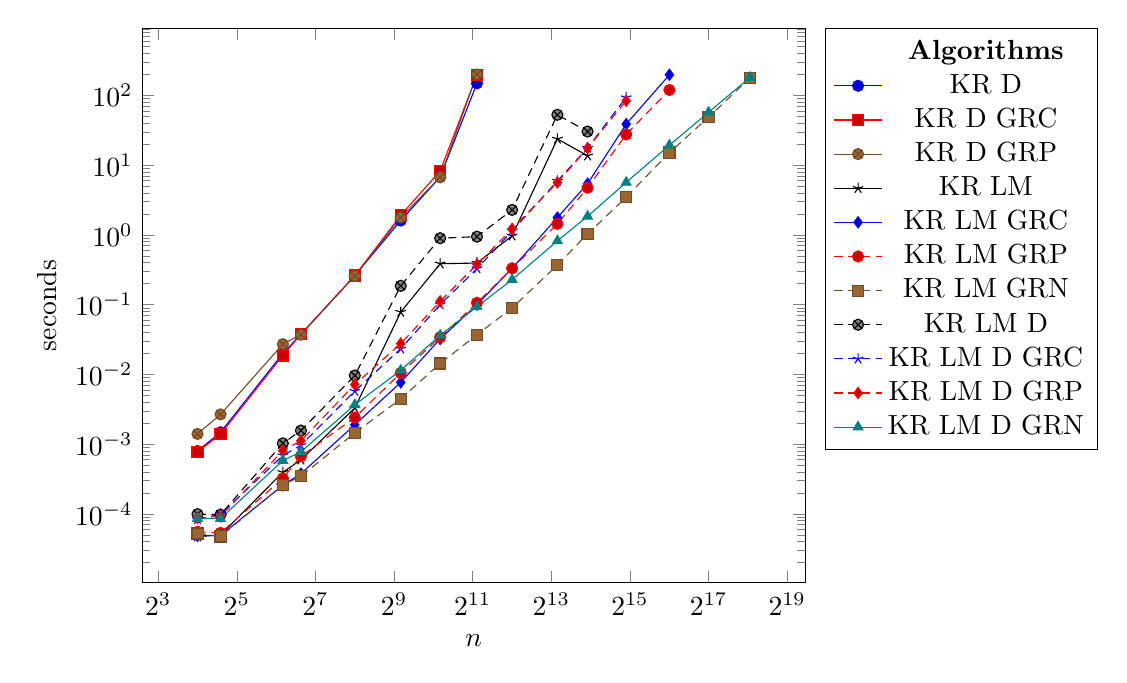
\begin{tikzpicture}
\begin{axis}[
    xlabel=$n$,ylabel=seconds,
    xmode=log,ymode=log,
    log basis x={2},
    legend style=
    {
        legend pos=outer north east
    },
    width=10cm
]
\addlegendimage{legend image code/.code=}
\legend{\textbf{Algorithms}, KR D, KR D GRC, KR D GRP, KR LM, KR LM GRC, KR LM GRP, KR LM GRN, KR LM D, KR LM D GRC, KR LM D GRP, KR LM D GRN}
\addplot table[x=n,y=value] {%KR
n value
16	0.000795004
24	0.00147618
72	0.019901867
99	0.037501367
256	0.260456667
575	1.606663333
1152	6.740186667
2205	149.337
};
\addplot table[x=n,y=value] {%KR GRC
n value
16	0.000769905
24	0.001389337
72	0.018663067
99	0.0377529
256	0.261381
575	1.908376667
1152	8.252073333
2205	197.4756667
};
\addplot table[x=n,y=value] {%KR GRP
n value
16	0.00139845
24	0.002666637
72	0.0271098
99	0.037121367
256	0.258182333
575	1.773686667
1152	6.72207
2205	200.141
};
\addplot table[x=n,y=value] {%KR LM
n value
16	4.70851E-05
24	4.97503E-05
72	0.000394004
99	0.000594782
256	0.003290843
575	0.078265033
1152	0.385737667
2205	0.395114667
4096	0.969813
9100	23.78033333
15488	13.6657
};
\addplot table[x=n,y=value] {%KR LM GRC
n value
16	4.81955E-05
24	4.90839E-05
72	0.000255858
99	0.000376681
256	0.001889957
575	0.007676197
1152	0.0321853
2205	0.099800333
4096	0.331238
9100	1.773373333
15488	5.421613333
30589	38.8194
65536	197.752
};
\addplot table[x=n,y=value] {%KR LM GRP
n value
16	5.53027E-05
24	5.31928E-05
72	0.000322266
99	0.000671628
256	0.002406003
575	0.010445347
1152	0.034050267
2205	0.10638
4096	0.331282667
9100	1.439603333
15488	4.751253333
30589	27.6015
65536	119.7773333
};
\addplot table[x=n,y=value] {%KR LM GRN
n value
16	5.21933E-05
24	4.73072E-05
72	0.000259523
99	0.000345365
256	0.001449643
575	0.00443921
1152	0.014312
2205	0.037018833
4096	0.089594333
9100	0.369817
15488	1.033306667
30589	3.473556667
65536	15.1593
130682	48.64013333
270848	178.9876667
};
\addplot table[x=n,y=value] {%KR LM D
n value
16	9.88343E-05
24	9.73907E-05
72	0.001024097
99	0.001562027
256	0.009612567
575	0.186065333
1152	0.896549
2205	0.943830667
4096	2.28156
9100	52.7981
15488	30.36093333
};
\addplot table[x=n,y=value] {%KR LM D GRC
n value
16	8.31763E-05
24	9.87233E-05
72	0.000685843
99	0.000960468
256	0.00575304
575	0.023246133
1152	0.100415667
2205	0.328566333
4096	1.139136667
9100	5.931156667
15488	17.6933
30589	93.37536667
};
\addplot table[x=n,y=value] {%KR LM D GRP
n value
16	8.69519E-05
24	9.19491E-05
72	0.000803777
99	0.001117273
256	0.007166817
575	0.027587633
1152	0.111327333
2205	0.376117333
4096	1.221456667
9100	5.651543333
15488	17.5763
30589	83.79273333
};
\addplot[mark=triangle*, teal] table[x=n,y=value] {%KR LM D GRN
n value
16	8.53971E-05
24	8.53972E-05
72	0.000580235
99	0.000774794
256	0.00366275
575	0.011421333
1152	0.036280633
2205	0.0934643
4096	0.228176333
9100	0.820808667
15488	1.847203333
30589	5.658126667
65536	19.2994
130682	57.2744
270848	180.989
};
\end{axis}
\end{tikzpicture}
\caption{King and Rao results from the GenRmf long graphs}
\label{fig:GenRmf long_KR_ResultsAppendix}
\end{figure}

%-----------------------------------------------------------------------------------------------------------
\clearpage


\subsection{Results from GenRmf flat graphs}
\begin{figure}[h]
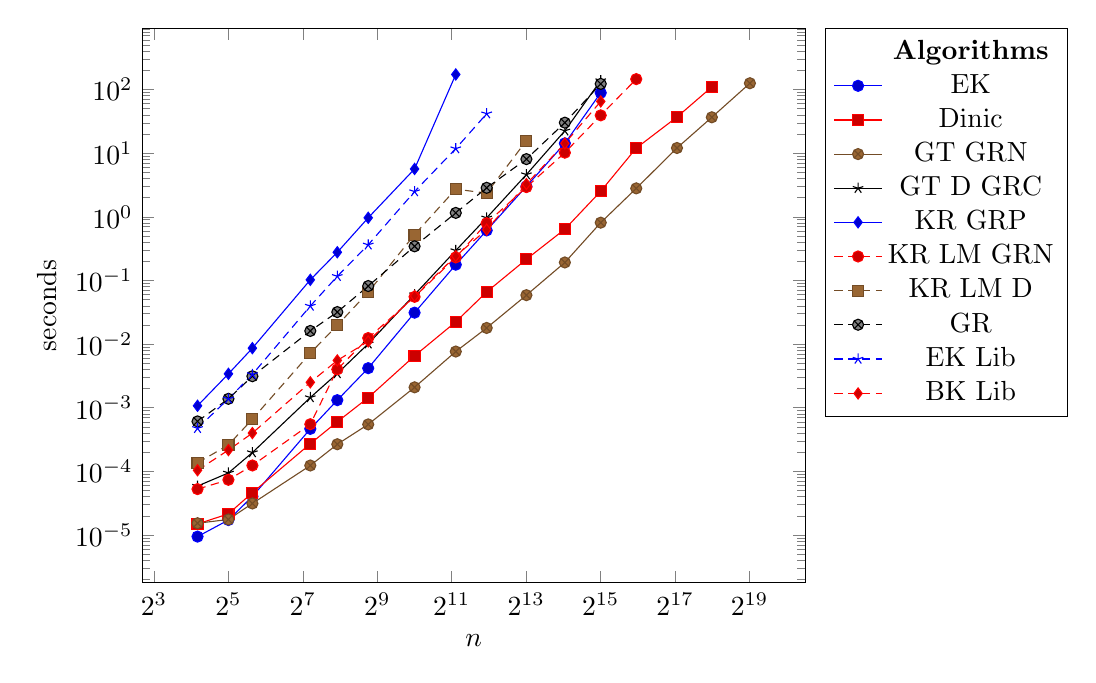
\begin{tikzpicture}
\begin{axis}[
    xlabel=$n$,ylabel=seconds,
    xmode=log,ymode=log,
    log basis x={2},
    legend style=
    {
        legend pos=outer north east
    },
    width=10cm
]
\addlegendimage{legend image code/.code=}
\legend{\textbf{Algorithms}, EK, Dinic, GT GRN, GT D GRC, KR GRP, KR LM GRN, KR LM D, GR, EK Lib, BK Lib}
\addplot table[x=n,y=value] {%EK
n value
18	9.4392E-06
32	1.72126E-05
50	4.03109E-05
147	0.000465408
243	0.001316157
432	0.00418523
1024	0.031191967
2205	0.176996333
3920	0.611422
8214	3.014606667
16807	14.2787
32768	88.94956667
};
\addplot table[x=n,y=value] {%Dinic
n value
18	1.48806E-05
32	2.15436E-05
50	4.61965E-05
147	0.000272404
243	0.000601443
432	0.001440867
1024	0.00653603
2205	0.022350033
3920	0.0660307
8214	0.215527667
16807	0.640137667
32768	2.524353333
63504	12.02686667
135531	36.99756667
259308	109.8443333
};
\addplot table[x=n,y=value] {%GT GRN
n value
18	1.53249E-05
32	1.75459E-05
50	0.000031316
147	0.00012371
243	0.000266963
432	0.000547475
1024	0.002093063
2205	0.007644327
3920	0.017937867
8214	0.0587656
16807	0.191883
32768	0.809820333
63504	2.801476667
135531	12.06703333
259308	36.68086667
526904	125.7226667
};
\addplot table[x=n,y=value] {%GT D GRC
n value
18	5.87453E-05
32	9.45034E-05
50	0.000197669
147	0.001447867
243	0.003451533
432	0.010111967
1024	0.059864533
2205	0.295727
3920	0.963905
8214	4.61783
16807	22.47756667
32768	138.508
};
\addplot table[x=n,y=value] {%KR GRP
n value
18	0.001074073
32	0.003409223
50	0.008633337
147	0.102404
243	0.277406
432	0.965820667
1024	5.656363333
2205	172.7583333
};
\addplot table[x=n,y=value] {%KR LM GRN
n value
18	5.26376E-05
32	0.000073737
50	0.00012382
147	0.000550917
243	0.004011667
432	0.012442333
1024	0.055324933
2205	0.230305333
3920	0.794109
8214	2.930473333
16807	10.18923333
32768	39.32803333
63504	145.8696667
};
\addplot table[x=n,y=value] {%KR LM D
n value
18	0.000136036
32	0.000260523
50	0.000661301
147	0.007218563
243	0.019773733
432	0.0653776
1024	0.525896
2205	2.72503
3920	2.35291
8214	15.7247
};
\addplot table[x=n,y=value] {%GR
n value
18	0.000610216
32	0.00138123
50	0.003127593
147	0.016109833
243	0.031885167
432	0.0818089
1024	0.343863333
2205	1.153163333
3920	2.85746
8214	8.068233333
16807	30.1861
32768	122.866
};
\addplot table[x=n,y=value] {%EK Lib
n value
18	0.000475183
32	0.001380687
50	0.00333872
147	0.039699067
243	0.116443333
432	0.363236333
1024	2.4961
2205	11.80336667
3920	41.74636667
};
\addplot table[x=n,y=value] {%BK Lib
n value
18	0.000104054
32	0.000215992
50	0.00039978
147	0.002510063
243	0.005535177
432	0.0110366
1024	0.0570666
2205	0.242166333
3920	0.629387
8214	3.27575
16807	14.24913333
32768	65.0965
};
\end{axis}
\end{tikzpicture}
\caption{Best and worst results from the GenRmf flat graphs}
\label{fig:GenRmf flat_BW_Results}
\end{figure}


\begin{figure}[h]
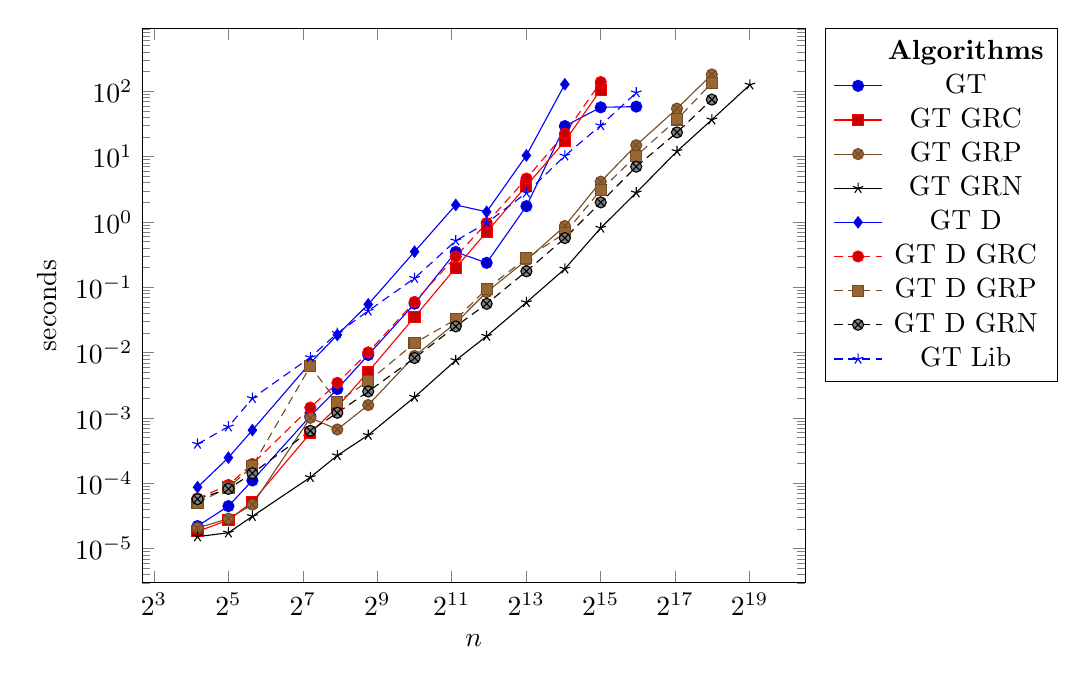
\begin{tikzpicture}
\begin{axis}[
    xlabel=$n$,ylabel=seconds,
    xmode=log,ymode=log,
    log basis x={2},
    legend style=
    {
        legend pos=outer north east
    },
    width=10cm
]
\addlegendimage{legend image code/.code=}
\legend{\textbf{Algorithms}, GT, GT GRC, GT GRP, GT GRN, GT D, GT D GRC, GT D GRP, GT D GRN, GT Lib}
\addplot table[x=n,y=value] {%GT
n value
18	2.22099E-05
32	4.48639E-05
50	0.000110827
147	0.001072623
243	0.002777677
432	0.009227643
1024	0.056178767
2205	0.347710667
3920	0.236927
8214	1.74571
16807	29.33203333
32768	56.85273333
63504	58.28513333
};
\addplot table[x=n,y=value] {%GT GRC
n value
18	1.84342E-05
32	2.74292E-05
50	5.23042E-05
147	0.000586896
243	0.001477067
432	0.00509139
1024	0.035166767
2205	0.199472
3920	0.702958333
8214	3.58601
16807	17.21576667
32768	105.3156667
};
\addplot table[x=n,y=value] {%GT GRP
n value
18	2.07662E-05
32	2.88728E-05
50	4.7307E-05
147	0.001008216
243	0.000668406
432	0.001579343
1024	0.008907267
2205	0.0284375
3920	0.084576833
8214	0.260927667
16807	0.868911
32768	4.137436667
63504	14.96233333
135531	54.3359
259308	181.0383333
};
\addplot table[x=n,y=value] {%GT GRN
n value
18	1.53249E-05
32	1.75459E-05
50	0.000031316
147	0.00012371
243	0.000266963
432	0.000547475
1024	0.002093063
2205	0.007644327
3920	0.017937867
8214	0.0587656
16807	0.191883
32768	0.809820333
63504	2.801476667
135531	12.06703333
259308	36.68086667
526904	125.7226667
};
\addplot table[x=n,y=value] {%GT D
n value
18	8.7396E-05
32	0.000247641
50	0.000652417
147	0.0069717
243	0.018692567
432	0.054880833
1024	0.351534
2205	1.823923333
3920	1.4308
8214	10.43303333
16807	127.9706667
};
\addplot table[x=n,y=value] {%GT D GRC
n value
18	5.87453E-05
32	9.45034E-05
50	0.000197669
147	0.001447867
243	0.003451533
432	0.010111967
1024	0.059864533
2205	0.295727
3920	0.963905
8214	4.61783
16807	22.47756667
32768	138.508
};
\addplot table[x=n,y=value] {%GT D GRP
n value
18	5.07497E-05
32	8.62856E-05
50	0.000182565
147	0.00619224
243	0.00176569
432	0.003644983
1024	0.014012367
2205	0.032288
3920	0.095217433
8214	0.279258333
16807	0.672308333
32768	3.07767
63504	10.2616
135531	37.05286667
259308	134.3013333
};
\addplot table[x=n,y=value] {%GT D GRN
n value
18	5.74127E-05
32	8.23989E-05
50	0.000143032
147	0.000637869
243	0.001202003
432	0.00254581
1024	0.008284307
2205	0.025236567
3920	0.056017433
8214	0.176041667
16807	0.567211
32768	1.995766667
63504	7.020556667
135531	23.4784
259308	74.6085
};
\addplot table[x=n,y=value] {%GT Lib
n value
18	0.000400113
32	0.000736262
50	0.00200534
147	0.008467563
243	0.019826867
432	0.043577133
1024	0.137993667
2205	0.516753333
3920	0.966842
8214	2.78562
16807	10.30583333
32768	29.97566667
63504	95.17936667
};
\end{axis}
\end{tikzpicture}
\caption{Goldberg and Tarjan results from the GenRmf flat graphs}
\label{fig:GenRmf flat_GT_Results}
\end{figure}


\begin{figure}[h]
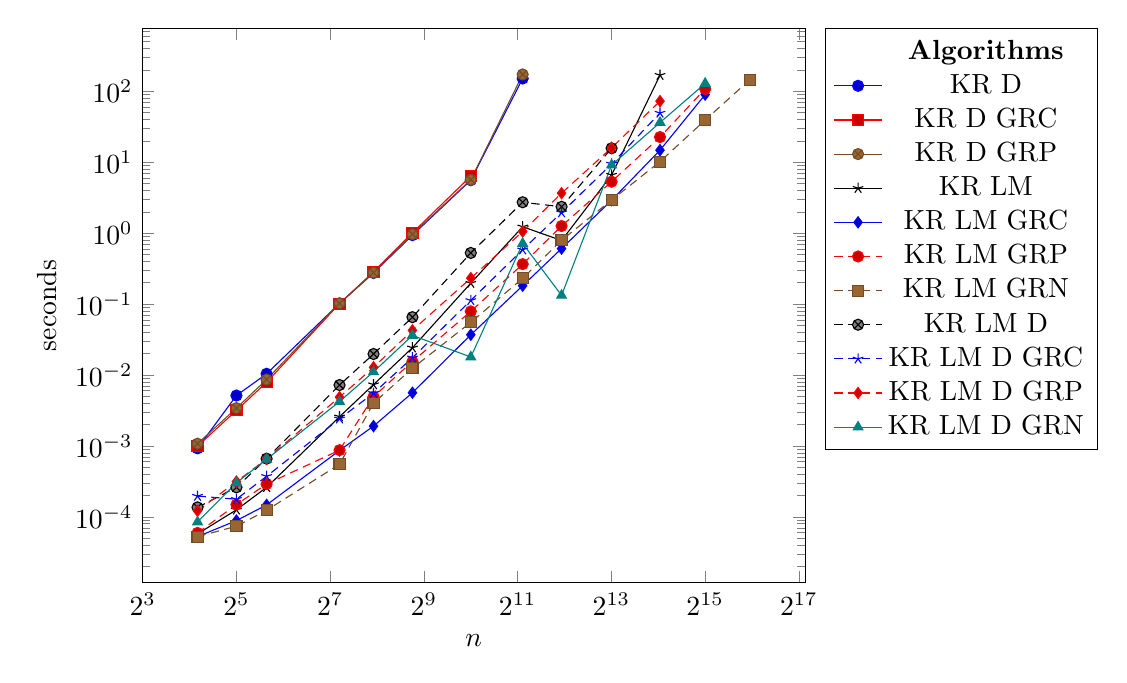
\begin{tikzpicture}
\begin{axis}[
    xlabel=$n$,ylabel=seconds,
    xmode=log,ymode=log,
    log basis x={2},
    legend style=
    {
        legend pos=outer north east
    },
    width=10cm
]
\addlegendimage{legend image code/.code=}
\legend{\textbf{Algorithms}, KR D, KR D GRC, KR D GRP, KR LM, KR LM GRC, KR LM GRP, KR LM GRN, KR LM D, KR LM D GRC, KR LM D GRP, KR LM D GRN}
\addplot table[x=n,y=value] {%KR
n value
18	0.000924822
32	0.005135713
50	0.010398667
147	0.1019604
243	0.274302333
432	0.936981667
1024	5.575076667
2205	151.3853333
};
\addplot table[x=n,y=value] {%KR GRC
n value
18	0.000991894
32	0.0031699
50	0.00789183
147	0.101455
243	0.285877333
432	1.00962
1024	6.366356667
};
\addplot table[x=n,y=value] {%KR GRP
n value
18	0.001074073
32	0.003409223
50	0.008633337
147	0.102404
243	0.277406
432	0.965820667
1024	5.656363333
2205	172.7583333
};
\addplot table[x=n,y=value] {%KR LM
n value
18	5.74127E-05
32	0.000125597
50	0.000260411
147	0.002579683
243	0.0073245
432	0.024196833
1024	0.197125667
2205	1.23007
3920	0.787139667
8214	6.59962
16807	168.589
};
\addplot table[x=n,y=value] {%KR LM GRC
n value
18	5.26375E-05
32	8.85064E-05
50	0.000147363
147	0.000863189
243	0.001903393
432	0.00562644
1024	0.036906367
2205	0.181411333
3920	0.605830667
8214	2.91064
16807	14.7904
32768	89.8431
};
\addplot table[x=n,y=value] {%KR LM GRP
n value
18	5.93005E-05
32	0.000149029
50	0.000290284
147	0.000871407
243	0.00495037
432	0.015484133
1024	0.078886133
2205	0.365700333
3920	1.26005
8214	5.312396667
16807	22.63123333
32768	107.989
};
\addplot table[x=n,y=value] {%KR LM GRN
n value
18	5.26376E-05
32	0.000073737
50	0.00012382
147	0.000550917
243	0.004011667
432	0.012442333
1024	0.055324933
2205	0.230305333
3920	0.794109
8214	2.930473333
16807	10.18923333
32768	39.32803333
63504	145.8696667
};
\addplot table[x=n,y=value] {%KR LM D
n value
18	0.000136036
32	0.000260523
50	0.000661301
147	0.007218563
243	0.019773733
432	0.0653776
1024	0.525896
2205	2.72503
3920	2.35291
8214	15.7247
};
\addplot table[x=n,y=value] {%KR LM D GRC
n value
18	0.000196224
32	0.000177235
50	0.000373349
147	0.002416107
243	0.005545263
432	0.017499567
1024	0.112657
2205	0.583763667
3920	1.945043333
8214	9.460863333
16807	49.42546667
};
\addplot table[x=n,y=value] {%KR LM D GRP
n value
18	0.000121488
32	0.000314382
50	0.00065486
147	0.00486675
243	0.0128281
432	0.042627733
1024	0.232225
2205	1.053173333
3920	3.663543333
8214	15.96356667
16807	72.6246
};
\addplot[mark=triangle*, teal] table[x=n,y=value] {%KR LM D GRN
n value
18	8.47309E-05
32	0.000302277
50	0.000648308
147	0.00421978
243	0.0110721
432	0.036097033
1024	0.017925533
2205	0.714243333
3920	0.132640667
8214	9.112416667
16807	36.27683333
32768	128.902
};
\end{axis}
\end{tikzpicture}
\caption{King and Rao results from the GenRmf flat graphs}
\label{fig:GenRmf flat_KR_Results}
\end{figure}

%-----------------------------------------------------------------------------------------------------------
\clearpage


\subsection{Results from GenRmf square graphs}
\begin{figure}[h]
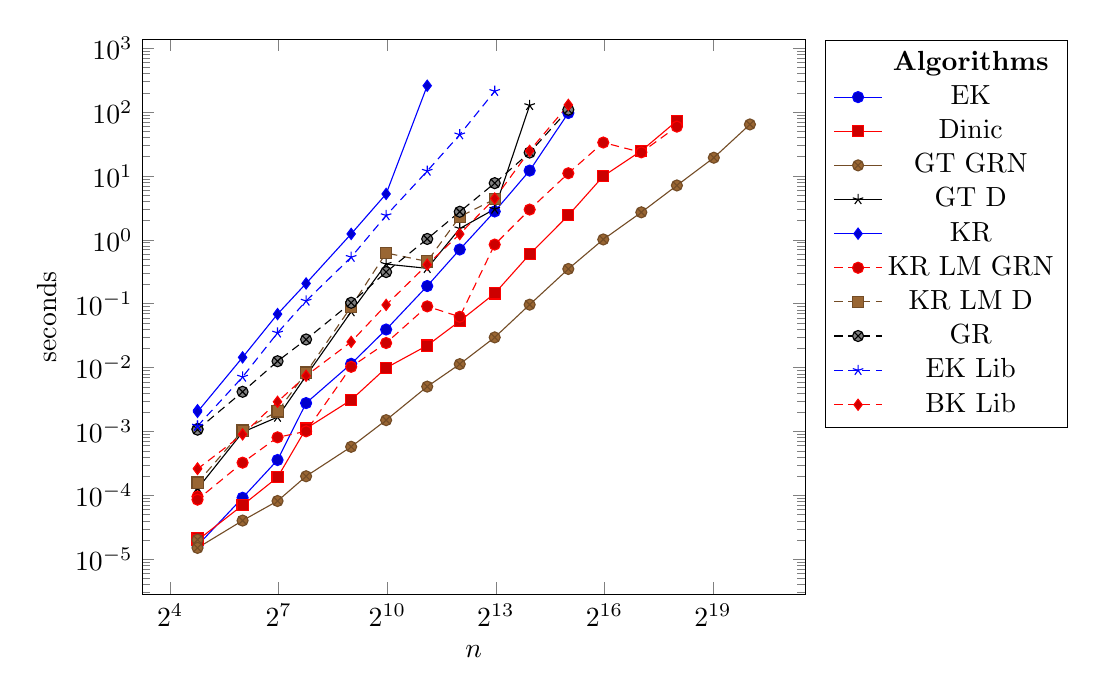
\begin{tikzpicture}
\begin{axis}[
    xlabel=$n$,ylabel=seconds,
    xmode=log,ymode=log,
    log basis x={2},
    legend style=
    {
        legend pos=outer north east
    },
    width=10cm
]
\addlegendimage{legend image code/.code=}
\legend{\textbf{Algorithms}, EK, Dinic, GT GRN, GT D, KR, KR LM GRN, KR LM D, GR, EK Lib, BK Lib}
\addplot table[x=n,y=value] {%EK
n value
27	1.83E-05
27	1.64353E-05
64	9.19488E-05
125	0.000358578
216	0.002789337
512	0.011478267
1000	0.039519567
2197	0.189271
4096	0.706506333
8000	2.78247
15625	12.12773333
32768	96.6569
};
\addplot table[x=n,y=value] {%Dinic
n value
27	2.16546E-05
27	1.98778E-05
64	7.04053E-05
125	0.000192226
216	0.001115157
512	0.003119373
1000	0.00991604
2197	0.0221898
4096	0.053542767
8000	0.144866667
15625	0.59337
32768	2.4171
64000	9.927513333
132651	24.71566667
262144	72.89203333
};
\addplot table[x=n,y=value] {%GT GRN
n value
27	2.03E-05
27	1.51027E-05
64	4.04221E-05
125	8.18436E-05
216	0.000199778
512	0.000577347
1000	0.001509167
2197	0.005050763
4096	0.0113486
8000	0.0297681
15625	0.096823533
32768	0.350279
64000	1.014996667
132651	2.6983
262144	7.101253333
531441	19.29156667
1061208	64.0214
};
\addplot table[x=n,y=value] {%GT D
n value
27	1.33E-04
27	0.000127152
64	0.000977459
125	0.00168207
216	0.007420783
512	0.0751745
1000	0.417246
2197	0.358329333
4096	1.503013333
8000	3.035766667
15625	127.1716667
};
\addplot table[x=n,y=value] {%KR
n value
27	2.16E-03
27	0.002033977
64	0.0144907
125	0.0688899
216	0.207899
512	1.23922
1000	5.23004
2197	258.178
};
\addplot table[x=n,y=value] {%KR LM GRN
n value
27	9.63E-05
27	8.59525E-05
64	0.000325931
125	0.000811551
216	0.001009107
512	0.010306333
1000	0.0242879
2197	0.090985567
4096	0.062492867
8000	0.84353
15625	2.978673333
32768	11.0194
64000	33.353
132651	23.40396667
262144	59.15526667
};
\addplot table[x=n,y=value] {%KR LM D
n value
27	1.61E-04
27	0.000158246
64	0.001037093
125	0.002061527
216	0.008381697
512	0.089949433
1000	0.622961333
2197	0.459367667
4096	2.298873333
8000	4.334706667
};
\addplot table[x=n,y=value] {%GR
n value
27	1.10E-03
27	0.00107007
64	0.004186893
125	0.0125998
216	0.027625867
512	0.103603333
1000	0.313361667
2197	1.03351
4096	2.753226667
8000	7.715346667
15625	23.232
32768	108.9246667
};
\addplot table[x=n,y=value] {%EK Lib
n value
27	0.001224103
27	0.001216997
64	0.007149513
125	0.0350155
216	0.110498333
512	0.535476
1000	2.40563
2197	11.93883333
4096	44.25053333
8000	211.9366667
};
\addplot table[x=n,y=value] {%BK Lib
n value
27	0.000264632
27	0.000259413
64	0.000902392
125	0.002922727
216	0.007462453
512	0.025325933
1000	0.095990433
2197	0.408633667
4096	1.230866667
8000	4.441643333
15625	24.72616667
32768	129.544
};
\end{axis}
\end{tikzpicture}
\caption{Best and worst results from the GenRmf square graphs}
\label{fig:GenRmf square_BW_ResultsAppendix}
\end{figure}


\begin{figure}[h]
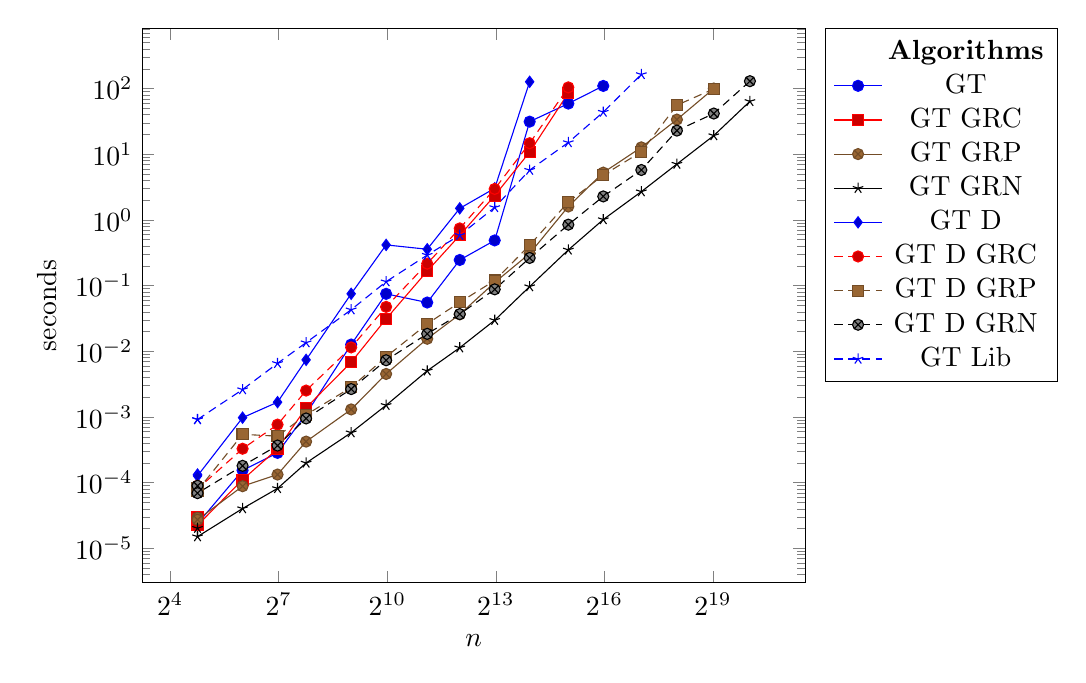
\begin{tikzpicture}
\begin{axis}[
    xlabel=$n$,ylabel=seconds,
    xmode=log,ymode=log,
    log basis x={2},
    legend style=
    {
        legend pos=outer north east
    },
    width=10cm
]
\addlegendimage{legend image code/.code=}
\legend{\textbf{Algorithms}, GT, GT GRC, GT GRP, GT GRN, GT D, GT D GRC, GT D GRP, GT D GRN, GT Lib}
\addplot table[x=n,y=value] {%GT
n value
27	2.54E-05
27	2.37646E-05
64	0.000153914
125	0.000284286
216	0.00111416
512	0.0126945
1000	0.075073033
2197	0.055363333
4096	0.245961333
8000	0.488409
15625	31.41703333
32768	59.17186667
64000	109.8606667
};
\addplot table[x=n,y=value] {%GT GRC
n value
27	3.03E-05
27	2.2432E-05
64	0.00011116
125	0.000326596
216	0.001382787
512	0.00682398
1000	0.031213833
2197	0.16648
4096	0.583621333
8000	2.351263333
15625	10.812
32768	85.61236667
};
\addplot table[x=n,y=value] {%GT GRP
n value
27	2.93E-05
27	2.73182E-05
64	8.83953E-05
125	0.000133037
216	0.000422432
512	0.00130516
1000	0.004525817
2197	0.0155378
4096	0.036563667
8000	0.111814333
15625	0.307891
32768	1.603586667
64000	5.25922
132651	12.75386667
262144	33.78733333
531441	100.2623333
};
\addplot table[x=n,y=value] {%GT GRN
n value
27	2.03E-05
27	1.51027E-05
64	4.04221E-05
125	8.18436E-05
216	0.000199778
512	0.000577347
1000	0.001509167
2197	0.005050763
4096	0.0113486
8000	0.0297681
15625	0.096823533
32768	0.350279
64000	1.014996667
132651	2.6983
262144	7.101253333
531441	19.29156667
1061208	64.0214
};
\addplot table[x=n,y=value] {%GT D
n value
27	1.33E-04
27	0.000127152
64	0.000977459
125	0.00168207
216	0.007420783
512	0.0751745
1000	0.417246
2197	0.358329333
4096	1.503013333
8000	3.035766667
15625	127.1716667
};
\addplot table[x=n,y=value] {%GT D GRC
n value
27	8.95E-05
27	8.04E-05
64	0.000328818
125	0.000766354
216	0.002527713
512	0.0114739
1000	0.0475249
2197	0.216508333
4096	0.744132
8000	2.9685
15625	14.74123333
32768	104.462
};
\addplot table[x=n,y=value] {%GT D GRP
n value
27	8.15E-05
27	7.59579E-05
64	0.000544588
125	0.000511051
216	0.001081957
512	0.002827437
1000	0.008248543
2197	0.026213167
4096	0.055797467
8000	0.119685667
15625	0.412618667
32768	1.87621
64000	4.814616667
132651	10.91256667
262144	55.88503333
531441	99.03183333
};
\addplot table[x=n,y=value] {%GT D GRN
n value
27	8.98E-05
27	0.000069295
64	0.000180789
125	0.000367908
216	0.000950806
512	0.00266219
1000	0.00731351
2197	0.018466767
4096	0.036885933
8000	0.0878232
15625	0.264105667
32768	0.848473667
64000	2.283013333
132651	5.76648
262144	22.9456
531441	41.73593333
1061208	129.805
};
\addplot table[x=n,y=value] {%GT Lib
n value
27	0.000922159
27	0.000915052
64	0.002620227
125	0.006562393
216	0.013568533
512	0.043020667
1000	0.114954
2197	0.291912667
4096	0.586437667
8000	1.553093333
15625	5.743833333
32768	15.12613333
64000	43.95683333
132651	164.3336667
};
\end{axis}
\end{tikzpicture}
\caption{Goldberg and Tarjan results from the GenRmf square graphs}
\label{fig:GenRmf square_GT_ResultsAppendix}
\end{figure}


\begin{figure}[h]
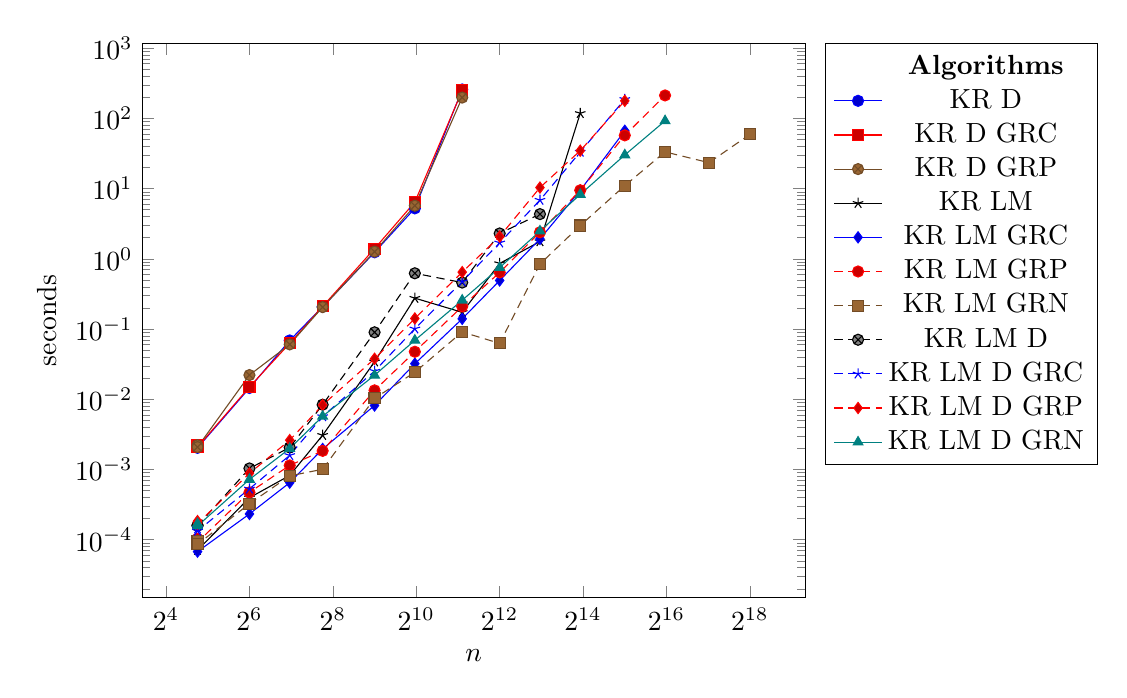
\begin{tikzpicture}
\begin{axis}[
    xlabel=$n$,ylabel=seconds,
    xmode=log,ymode=log,
    log basis x={2},
    legend style=
    {
        legend pos=outer north east
    },
    width=10cm
]
\addlegendimage{legend image code/.code=}
\legend{\textbf{Algorithms}, KR D, KR D GRC, KR D GRP, KR LM, KR LM GRC, KR LM GRP, KR LM GRN, KR LM D, KR LM D GRC, KR LM D GRP, KR LM D GRN}
\addplot table[x=n,y=value] {%KR
n value
27	2.16E-03
27	0.002033977
64	0.0144907
125	0.0688899
216	0.207899
512	1.23922
1000	5.23004
2197	258.178
};
\addplot table[x=n,y=value] {%KR GRC
n value
27	2.23E-03
27	0.00208284
64	0.014971033
125	0.062672033
216	0.210346
512	1.397736667
1000	6.43309
2197	249.9376667
};
\addplot table[x=n,y=value] {%KR GRP
n value
27	2.22E-03
27	0.002085847
64	0.022137767
125	0.060497533
216	0.205200667
512	1.26544
1000	5.717356667
2197	198.016
};
\addplot table[x=n,y=value] {%KR LM
n value
27	7.78E-05
27	7.11828E-05
64	0.000396225
125	0.000823766
216	0.003079187
512	0.034277133
1000	0.275727667
2197	0.173293667
4096	0.859855333
8000	1.765033333
15625	118.149
};
\addplot table[x=n,y=value] {%KR LM GRC
n value
27	7.58E-05
27	6.77403E-05
64	0.000232871
125	0.000650307
216	0.00196269
512	0.008164487
1000	0.0320805
2197	0.139880333
4096	0.492149333
8000	1.92034
15625	9.41052
32768	66.65046667
};
\addplot table[x=n,y=value] {%KR LM GRP
n value
27	1.03E-04
27	9.21711E-05
64	0.000473294
125	0.001145363
216	0.00184309
512	0.013407133
1000	0.047549267
2197	0.209707
4096	0.641041333
8000	2.392316667
15625	9.472133333
32768	57.29816667
64000	212.2696667
};
\addplot table[x=n,y=value] {%KR LM GRN
n value
27	9.63E-05
27	8.59525E-05
64	0.000325931
125	0.000811551
216	0.001009107
512	0.010306333
1000	0.0242879
2197	0.090985567
4096	0.062492867
8000	0.84353
15625	2.978673333
32768	11.0194
64000	33.353
132651	23.40396667
262144	59.15526667
};
\addplot table[x=n,y=value] {%KR LM D
n value
27	1.61E-04
27	0.000158246
64	0.001037093
125	0.002061527
216	0.008381697
512	0.089949433
1000	0.622961333
2197	0.459367667
4096	2.298873333
8000	4.334706667
};
\addplot table[x=n,y=value] {%KR LM D GRC
n value
27	1.43E-04
27	0.000133593
64	0.000530595
125	0.001592453
216	0.005694627
512	0.025246367
1000	0.100972333
2197	0.473784333
4096	1.692813333
8000	6.861693333
15625	33.215
32768	187.0353333
};
\addplot table[x=n,y=value] {%KR LM D GRP
n value
27	1.84E-04
27	0.000169795
64	0.000882734
125	0.00262177
216	0.008297853
512	0.037802967
1000	0.141620333
2197	0.646652
4096	2.074956667
8000	10.3482
15625	34.67336667
32768	177.815
};
\addplot[mark=triangle*, teal] table[x=n,y=value] {%KR LM D GRN
n value
27	1.70E-04
27	0.000157357
64	0.0007226
125	0.001988787
216	0.005735383
512	0.022002833
1000	0.0692056
2197	0.257478
4096	0.750494333
8000	2.48334
15625	8.26
32768	30.14693333
64000	92.17513333
};
\end{axis}
\end{tikzpicture}
\caption{King and Rao results from the GenRmf square graphs}
\label{fig:GenRmf square_KR_Results}
\end{figure}

%-----------------------------------------------------------------------------------------------------------
\clearpage


\subsection{Results from Wash long graphs}
\begin{figure}[h]
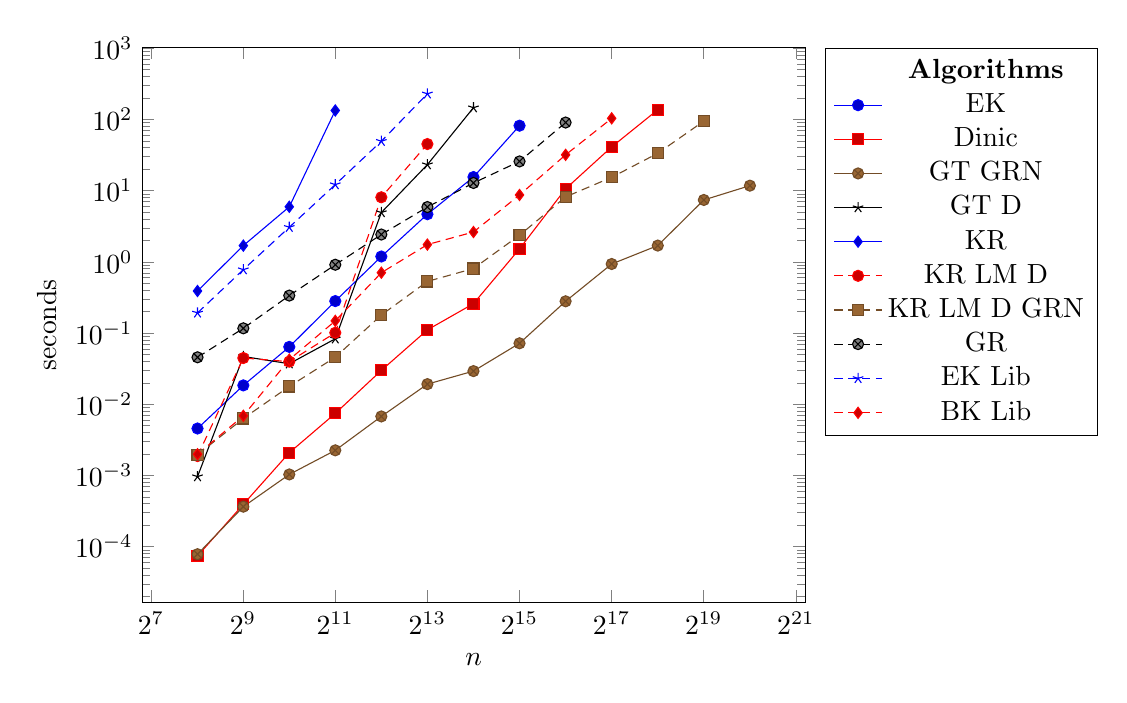
\begin{tikzpicture}
\begin{axis}[
    xlabel=$n$,ylabel=seconds,
    xmode=log,ymode=log,
    log basis x={2},
    legend style=
    {
        legend pos=outer north east
    },
    width=10cm
]
\addlegendimage{legend image code/.code=}
\legend{\textbf{Algorithms}, EK, Dinic, GT GRN, GT D, KR, KR LM D, KR LM D GRN, GR, EK Lib, BK Lib}
\addplot table[x=n,y=value] {%EK
n value
258	0.00455813
514	0.018388
1026	0.063829267
2050	0.280650667
4098	1.186396667
8194	4.660366667
16386	15.4853
32770	81.58816667
};
\addplot table[x=n,y=value] {%Dinic
n value
258	7.39589E-05
514	0.000392448
1026	0.00208284
2050	0.007431643
4098	0.0298423
8194	0.110588
16386	0.258280667
32770	1.520013333
65538	10.58663333
131074	41.0456
262146	136.5323333
};
\addplot table[x=n,y=value] {%GT GRN
n value
258	0.00007829
514	0.000364021
1026	0.00103243
2050	0.002250977
4098	0.00673583
8194	0.0191461
16386	0.029171
32770	0.071709467
65538	0.278762667
131074	0.931172
262146	1.689216667
524290	7.384293333
1048576	11.7299
};
\addplot table[x=n,y=value] {%GT D
n value
258	0.000963133
514	0.046797767
1026	0.037027933
2050	0.082945567
4098	4.91926
8194	23.14326667
16386	145.951
};
\addplot table[x=n,y=value] {%KR
n value
258	0.388986
514	1.687986667
1026	5.91655
2050	133.461
};
\addplot table[x=n,y=value] {%KR LM D
n value
258	0.001871523
514	0.044522067
1026	0.0396492
2050	0.100842
4098	8.054103333
8194	45.0224
};
\addplot table[x=n,y=value] {%KR LM D GRN
n value
258	0.001956473
514	0.006307733
1026	0.0177545
2050	0.045698067
4098	0.178866333
8194	0.530067
16386	0.803962667
32770	2.36107
65538	8.150896667
131074	15.36236667
262146	33.3926
524290	94.52643333
};
\addplot table[x=n,y=value] {%GR
n value
258	0.0455862
514	0.116387
1026	0.335383333
2050	0.909223667
4098	2.416166667
8194	5.87323
16386	12.79106667
32770	25.68216667
65538	90.29623333
};
\addplot table[x=n,y=value] {%EK Lib
n value
258	0.191596667
514	0.776001
1026	3.056936667
2050	12.1327
4098	49.3162
8194	228.5943333
};
\addplot table[x=n,y=value] {%BK Lib
n value
258	0.001984353
514	0.006870553
1026	0.0423145
2050	0.147986667
4098	0.702769333
8194	1.744473333
16386	2.61717
32770	8.679073333
65538	31.74643333
131074	103.3123333
};
\end{axis}
\end{tikzpicture}
\caption{Best and worst results from the Wash long graphs}
\label{fig:Wash long_BW_Results}
\end{figure}


\begin{figure}[h]
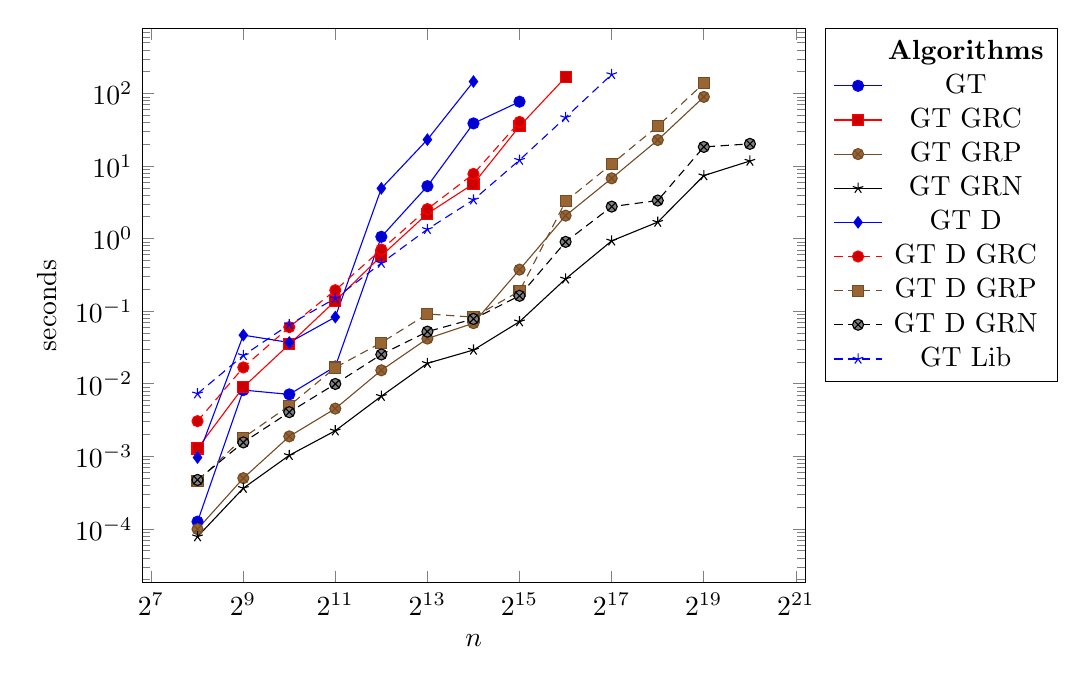
\begin{tikzpicture}
\begin{axis}[
    xlabel=$n$,ylabel=seconds,
    xmode=log,ymode=log,
    log basis x={2},
    legend style=
    {
        legend pos=outer north east
    },
    width=10cm
]
\addlegendimage{legend image code/.code=}
\legend{\textbf{Algorithms}, GT, GT GRC, GT GRP, GT GRN, GT D, GT D GRC, GT D GRP, GT D GRN, GT Lib}
\addplot table[x=n,y=value] {%GT
n value
258	0.000125819
514	0.008185667
1026	0.007138363
2050	0.017273933
4098	1.059973333
8194	5.279913333
16386	38.7052
32770	77.06073333
};
\addplot table[x=n,y=value] {%GT GRC
n value
258	0.001285393
514	0.008987553
1026	0.034958967
2050	0.138807
4098	0.579380667
8194	2.207283333
16386	5.693513333
32770	35.35053333
65538	167.6426667
};
\addplot table[x=n,y=value] {%GT GRP
n value
258	9.92782E-05
514	0.000500499
1026	0.00188184
2050	0.00454514
4098	0.015331
8194	0.041919
16386	0.068337667
32770	0.374196333
65538	2.072736667
131074	6.770743333
262146	22.8228
524290	89.71463333
};
\addplot table[x=n,y=value] {%GT GRN
n value
258	0.00007829
514	0.000364021
1026	0.00103243
2050	0.002250977
4098	0.00673583
8194	0.0191461
16386	0.029171
32770	0.071709467
65538	0.278762667
131074	0.931172
262146	1.689216667
524290	7.384293333
1048576	11.7299
};
\addplot table[x=n,y=value] {%GT D
n value
258	0.000963133
514	0.046797767
1026	0.037027933
2050	0.082945567
4098	4.91926
8194	23.14326667
16386	145.951
};
\addplot table[x=n,y=value] {%GT D GRC
n value
258	0.0030522
514	0.0168027
1026	0.0603235
2050	0.194416667
4098	0.707329333
8194	2.552136667
16386	7.796243333
32770	40.53683333
};
\addplot table[x=n,y=value] {%GT D GRP
n value
258	0.000453305
514	0.001807667
1026	0.00497547
2050	0.016712433
4098	0.036814533
8194	0.091586867
16386	0.082781533
32770	0.188612667
65538	3.26371
131074	10.66083333
262146	35.4517
524290	138.2766667
};
\addplot table[x=n,y=value] {%GT D GRN
n value
258	0.000472849
514	0.00155514
1026	0.00405964
2050	0.00993795
4098	0.025338533
8194	0.052303033
16386	0.0782536
32770	0.162790667
65538	0.901931333
131074	2.760933333
262146	3.348056667
524290	18.34756667
1048576	20.21003333
};
\addplot table[x=n,y=value] {%GT Lib
n value
258	0.007290433
514	0.024574033
1026	0.065415467
2050	0.150266333
4098	0.459179333
8194	1.343486667
16386	3.42729
32770	12.08016667
65538	46.69996667
131074	182.9003333
};
\end{axis}
\end{tikzpicture}
\caption{Goldberg and Tarjan results from the Wash long graphs}
\label{fig:Wash long_GT_Results}
\end{figure}


\begin{figure}[h]
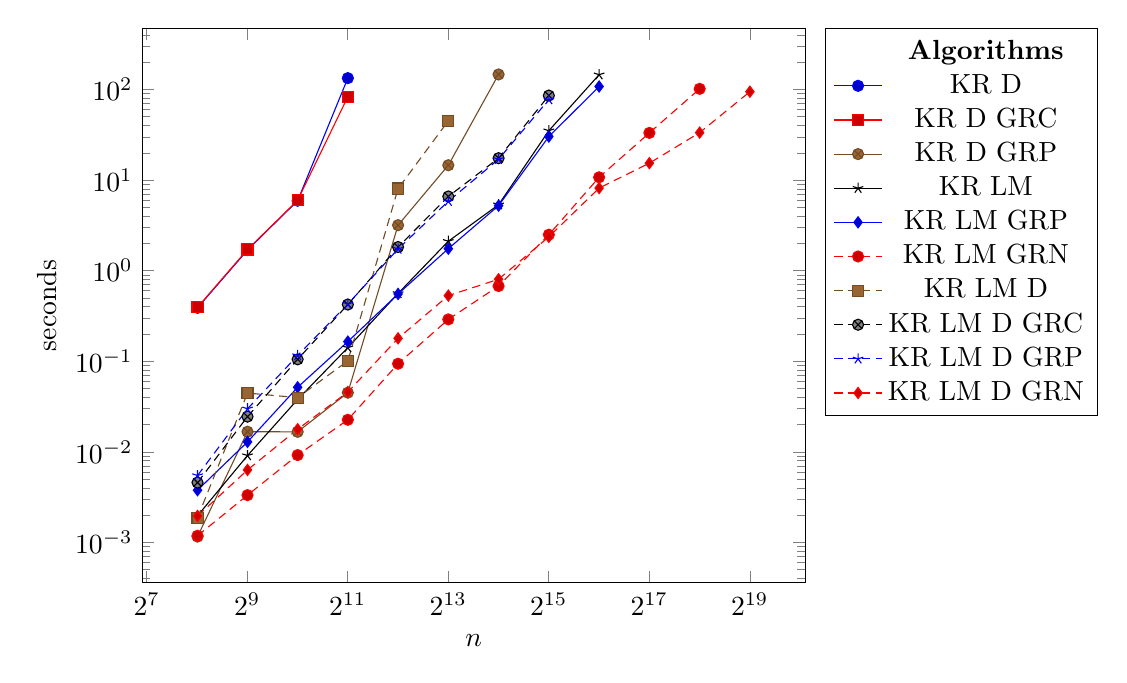
\begin{tikzpicture}
\begin{axis}[
    xlabel=$n$,ylabel=seconds,
    xmode=log,ymode=log,
    log basis x={2},
    legend style=
    {
        legend pos=outer north east
    },
    width=10cm
]
\addlegendimage{legend image code/.code=}
\legend{\textbf{Algorithms}, KR D, KR D GRC, KR D GRP, KR LM, KR LM GRP, KR LM GRN, KR LM D, KR LM D GRC, KR LM D GRP, KR LM D GRN}
\addplot table[x=n,y=value] {%KR
n value
258	0.388986
514	1.687986667
1026	5.91655
2050	133.461
};
\addplot table[x=n,y=value] {%KR GRP
n value
258	0.394335667
514	1.712723333
1026	5.980416667
2050	83.11296667
};
\addplot table[x=n,y=value] {%KR LM
n value
258	0.001158027
514	0.016664333
1026	0.0166107
2050	0.044975967
4098	3.17705
8194	14.57306667
16386	146.5643333
};
\addplot table[x=n,y=value] {%KR LM GRC
n value
258	0.0019678
514	0.00909097
1026	0.037847933
2050	0.141140667
4098	0.560116
8194	2.111113333
16386	5.345923333
32770	35.08333333
65538	145.6033333
};
\addplot table[x=n,y=value] {%KR LM GRP
n value
258	0.003771133
514	0.0128673
1026	0.051574
2050	0.164608333
4098	0.552708
8194	1.747106667
16386	5.22136
32770	30.23373333
65538	107.821
};
\addplot table[x=n,y=value] {%KR LM GRN
n value
258	0.001184233
514	0.003323717
1026	0.00919758
2050	0.022584967
4098	0.093840167
8194	0.289705333
16386	0.67618
32770	2.49438
65538	10.7308
131074	33.17436667
262146	101.676
};
\addplot table[x=n,y=value] {%KR LM D
n value
258	0.001871523
514	0.044522067
1026	0.0396492
2050	0.100842
4098	8.054103333
8194	45.0224
};
\addplot table[x=n,y=value] {%KR LM D GRC
n value
258	0.004577133
514	0.024459433
1026	0.104925
2050	0.422261
4098	1.82286
8194	6.58966
16386	17.44673333
32770	85.69343333
};
\addplot table[x=n,y=value] {%KR LM D GRP
n value
258	0.005469973
514	0.029860167
1026	0.115612667
2050	0.42751
4098	1.734793333
8194	5.83833
16386	16.96373333
32770	77.27503333
};
\addplot table[x=n,y=value] {%KR LM D GRN
n value
258	0.001956473
514	0.006307733
1026	0.0177545
2050	0.045698067
4098	0.178866333
8194	0.530067
16386	0.803962667
32770	2.36107
65538	8.150896667
131074	15.36236667
262146	33.3926
524290	94.52643333
};
\end{axis}
\end{tikzpicture}
\caption{King and Rao results from the Wash long graphs}
\label{fig:Wash long_KR_Results}
\end{figure}

%-----------------------------------------------------------------------------------------------------------
\clearpage


\subsection{Results from Wash wide graphs}
\begin{figure}[h]
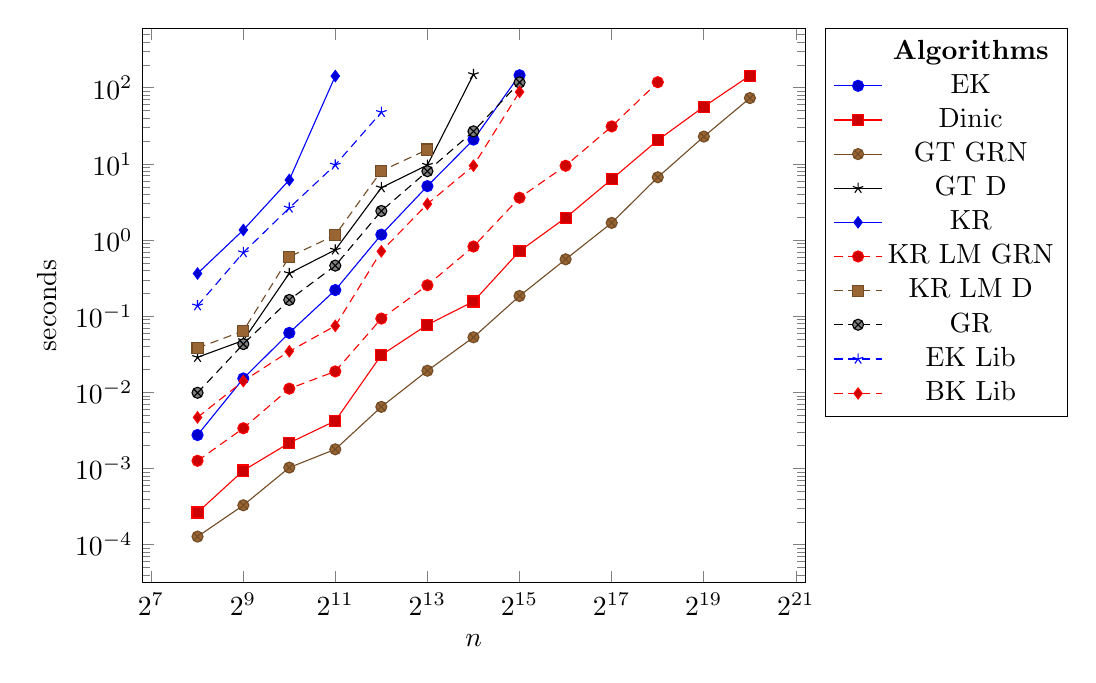
\begin{tikzpicture}
\begin{axis}[
    xlabel=$n$,ylabel=seconds,
    xmode=log,ymode=log,
    log basis x={2},
    legend style=
    {
        legend pos=outer north east
    },
    width=10cm
]
\addlegendimage{legend image code/.code=}
\legend{\textbf{Algorithms}, EK, Dinic, GT GRN, GT D, KR, KR LM GRN, KR LM D, GR, EK Lib, BK Lib}
\addplot table[x=n,y=value] {%EK
n value
258	0.00275391
514	0.0152435
1026	0.060453233
2050	0.220815
4098	1.178703333
8194	5.108153333
16386	20.86096667
32770	145.9943333
};
\addplot table[x=n,y=value] {%Dinic
n value
258	0.000264853
514	0.000941476
1026	0.002168793
2050	0.00422976
4098	0.030909467
8194	0.0773594
16386	0.156071667
32770	0.715507333
65538	1.959956667
131074	6.289176667
262146	20.50246667
524290	56.4742
1048578	144.392
};
\addplot table[x=n,y=value] {%GT GRN
n value
258	0.000127707
514	0.000329373
1026	0.001029652
2050	0.001789457
4098	0.00645676
8194	0.0192589
16386	0.052897167
32770	0.184429667
65538	0.559192
131074	1.680873333
262146	6.679286667
524290	22.85353333
1048578	73.2423
};
\addplot table[x=n,y=value] {%GT D
n value
258	0.028931
514	0.0480383
1026	0.366069
2050	0.743220667
4098	4.87707
8194	9.65479
16386	149.6193333
};
\addplot table[x=n,y=value] {%KR
n value
258	0.363904333
514	1.35767
1026	6.165536667
2050	142.452
};
\addplot table[x=n,y=value] {%KR LM GRN
n value
258	0.00126419
514	0.003382793
1026	0.011198767
2050	0.018873433
4098	0.0931617
8194	0.255151667
16386	0.822616667
32770	3.595813333
65538	9.45794
131074	31.09106667
262146	118.3703333
};
\addplot table[x=n,y=value] {%KR LM D
n value
258	0.038245967
514	0.064131167
1026	0.602363
2050	1.16391
4098	8.07734
8194	15.42616667
};
\addplot table[x=n,y=value] {%GR
n value
258	0.00988439
514	0.043069933
1026	0.163758333
2050	0.462004333
4098	2.41123
8194	8.02773
16386	26.78126667
32770	117.4263333
};
\addplot table[x=n,y=value] {%EK Lib
n value
258	0.137420667
514	0.686362333
1026	2.640513333
2050	9.708146667
4098	47.70486667
};
\addplot table[x=n,y=value] {%BK Lib
n value
258	0.00469564
514	0.014075633
1026	0.0346164
2050	0.074734567
4098	0.711892
8194	2.98372
16386	9.469473333
32770	88.19736667
};
\end{axis}
\end{tikzpicture}
\caption{Best and worst results from the Wash wide graphs}
\label{fig:Wash wide_BW_Results}
\end{figure}


\begin{figure}[h]
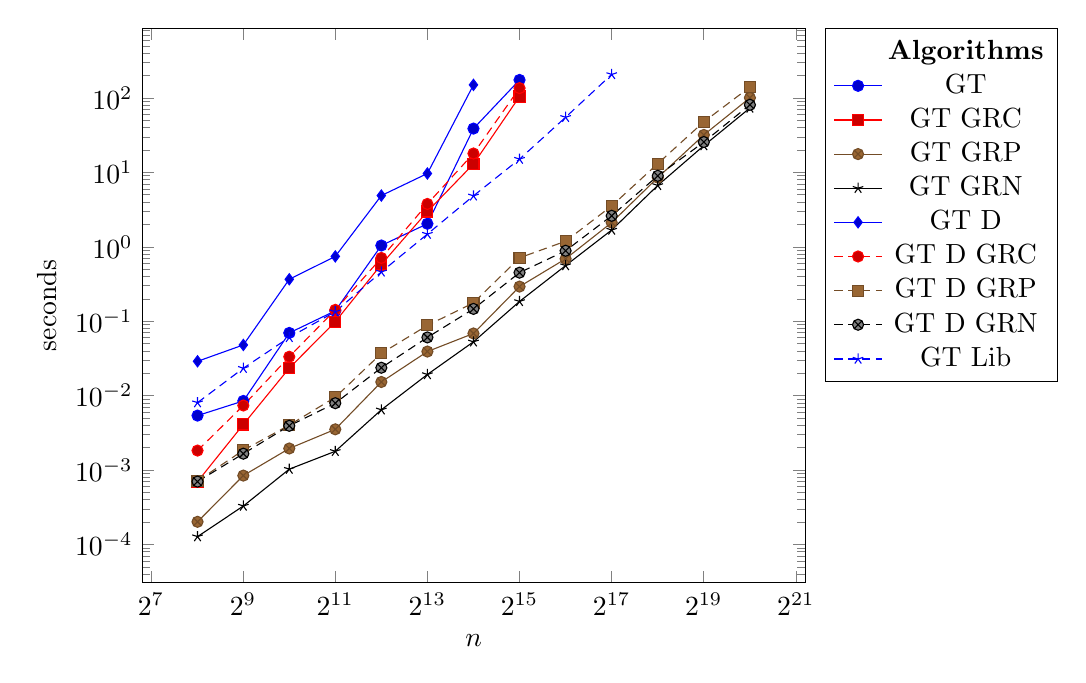
\begin{tikzpicture}
\begin{axis}[
    xlabel=$n$,ylabel=seconds,
    xmode=log,ymode=log,
    log basis x={2},
    legend style=
    {
        legend pos=outer north east
    },
    width=10cm
]
\addlegendimage{legend image code/.code=}
\legend{\textbf{Algorithms}, GT, GT GRC, GT GRP, GT GRN, GT D, GT D GRC, GT D GRP, GT D GRN, GT Lib}
\addplot table[x=n,y=value] {%GT
n value
258	0.005397887
514	0.00849272
1026	0.069627133
2050	0.137981667
4098	1.041136667
8194	2.039763333
16386	38.72533333
32770	174.4586667
};
\addplot table[x=n,y=value] {%GT GRC
n value
258	0.000700388
514	0.004106717
1026	0.0234676
2050	0.0985133
4098	0.578804
8194	2.978286667
16386	12.9586
32770	104.409
};
\addplot table[x=n,y=value] {%GT GRP
n value
258	0.000201999
514	0.000843642
1026	0.001951807
2050	0.00353048
4098	0.015270067
8194	0.0391442
16386	0.068477133
32770	0.291984
65538	0.689515
131074	2.116356667
262146	8.503033333
524290	31.83243333
1048578	100.3662333
};
\addplot table[x=n,y=value] {%GT GRN
n value
258	0.000127707
514	0.000329373
1026	0.001029652
2050	0.001789457
4098	0.00645676
8194	0.0192589
16386	0.052897167
32770	0.184429667
65538	0.559192
131074	1.680873333
262146	6.679286667
524290	22.85353333
1048578	73.2423
};
\addplot table[x=n,y=value] {%GT D
n value
258	0.028931
514	0.0480383
1026	0.366069
2050	0.743220667
4098	4.87707
8194	9.65479
16386	149.6193333
};
\addplot table[x=n,y=value] {%GT D GRC
n value
258	0.00182921
514	0.007377473
1026	0.0333401
2050	0.142173667
4098	0.708439333
8194	3.76566
16386	17.92476667
32770	135.5356667
};
\addplot table[x=n,y=value] {%GT D GRP
n value
258	0.000714938
514	0.001848203
1026	0.004024107
2050	0.00951629
4098	0.037023733
8194	0.087905367
16386	0.176312
32770	0.711375
65538	1.187876667
131074	3.542926667
262146	13.07743333
524290	47.78543333
1048578	140.107
};
\addplot table[x=n,y=value] {%GT D GRN
n value
258	0.000700724
514	0.001661527
1026	0.003936377
2050	0.007919837
4098	0.023725
8194	0.060609267
16386	0.146432
32770	0.449296
65538	0.884841667
131074	2.60916
262146	8.989773333
524290	25.54076667
1048578	80.799
};
\addplot table[x=n,y=value] {%GT Lib
n value
258	0.00805746
514	0.023360733
1026	0.060663733
2050	0.134216
4098	0.459610333
8194	1.481406667
16386	4.83742
32770	15.06266667
65538	54.98906667
131074	206.772
};
\end{axis}
\end{tikzpicture}
\caption{Goldberg and Tarjan results from the Wash wide graphs}
\label{fig:Wash wide_GT_Results}
\end{figure}


\begin{figure}[h]
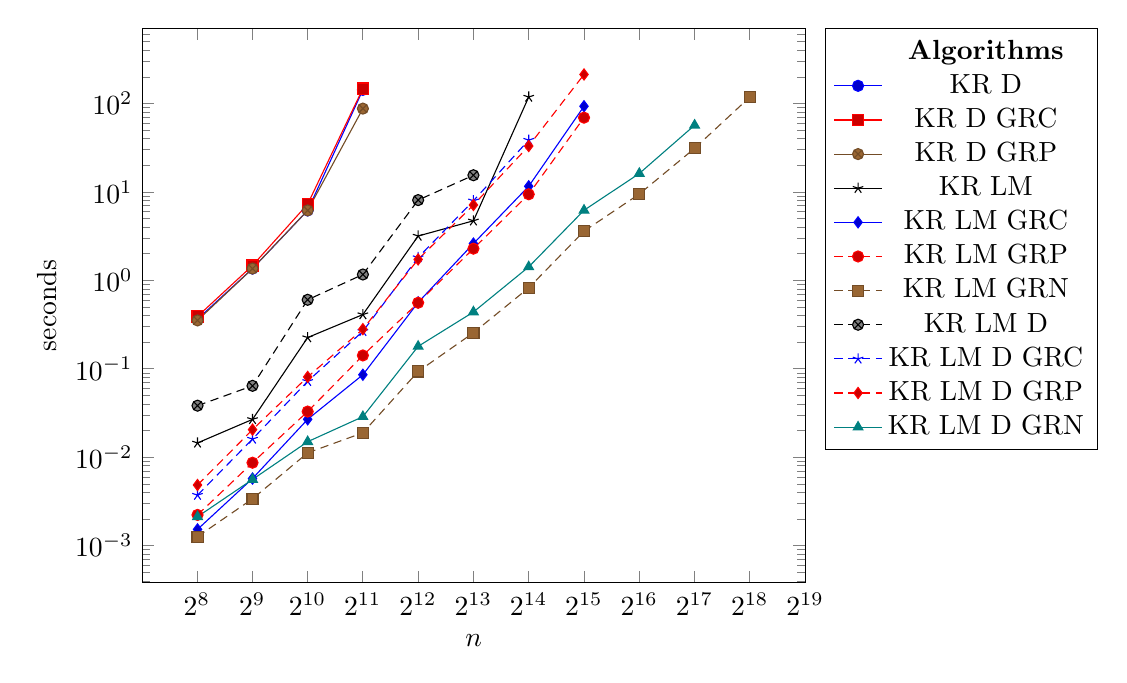
\begin{tikzpicture}
\begin{axis}[
    xlabel=$n$,ylabel=seconds,
    xmode=log,ymode=log,
    log basis x={2},
    legend style=
    {
        legend pos=outer north east
    },
    width=10cm
]
\addlegendimage{legend image code/.code=}
\legend{\textbf{Algorithms}, KR D, KR D GRC, KR D GRP, KR LM, KR LM GRC, KR LM GRP, KR LM GRN, KR LM D, KR LM D GRC, KR LM D GRP, KR LM D GRN}
\addplot table[x=n,y=value] {%KR
n value
258	0.363904333
514	1.35767
1026	6.165536667
2050	142.452
};
\addplot table[x=n,y=value] {%KR GRC
n value
258	0.390611333
514	1.4708
1026	7.269586667
2050	147.5433333
};
\addplot table[x=n,y=value] {%KR GRP
n value
258	0.352055333
514	1.358303333
1026	6.17634
2050	87.4755
};
\addplot table[x=n,y=value] {%KR LM
n value
258	0.014494433
514	0.0267644
1026	0.225451667
2050	0.410102
4098	3.170193333
8194	4.711013333
16386	118.326
};
\addplot table[x=n,y=value] {%KR LM GRC
n value
258	0.001526377
514	0.005739157
1026	0.026819933
2050	0.085569067
4098	0.562867
8194	2.602023333
16386	11.57923333
32770	92.96356667
};
\addplot table[x=n,y=value] {%KR LM GRP
n value
258	0.00222466
514	0.008658543
1026	0.0328203
2050	0.141411
4098	0.557627
8194	2.280763333
16386	9.398566667
32770	69.1255
};
\addplot table[x=n,y=value] {%KR LM GRN
n value
258	0.00126419
514	0.003382793
1026	0.011198767
2050	0.018873433
4098	0.0931617
8194	0.255151667
16386	0.822616667
32770	3.595813333
65538	9.45794
131074	31.09106667
262146	118.3703333
};
\addplot table[x=n,y=value] {%KR LM D
n value
258	0.038245967
514	0.064131167
1026	0.602363
2050	1.16391
4098	8.07734
8194	15.42616667
};
\addplot table[x=n,y=value] {%KR LM D GRC
n value
258	0.003725053
514	0.016062567
1026	0.0721805
2050	0.265253667
4098	1.81085
8194	7.93862
16386	38.531
};
\addplot table[x=n,y=value] {%KR LM D GRP
n value
258	0.00484776
514	0.020500433
1026	0.0808727
2050	0.280267333
4098	1.72412
8194	7.104583333
16386	32.9985
32770	212.8473333
};
\addplot[mark=triangle*, teal] table[x=n,y=value] {%KR LM D GRN
n value
258	0.002122937
514	0.005603013
1026	0.014965867
2050	0.028723433
4098	0.179154667
8194	0.438172
16386	1.418813333
32770	6.193153333
65538	16.14906667
131074	56.7592
};
\end{axis}
\end{tikzpicture}
\caption{King and Rao results from the Wash wide graphs}
\label{fig:Wash wide_KR_Results}
\end{figure}


%-----------------------------------------------------------------------------------------------------------
\clearpage


\subsection{Results from Computer Vision graphs}
\begin{figure}[h]
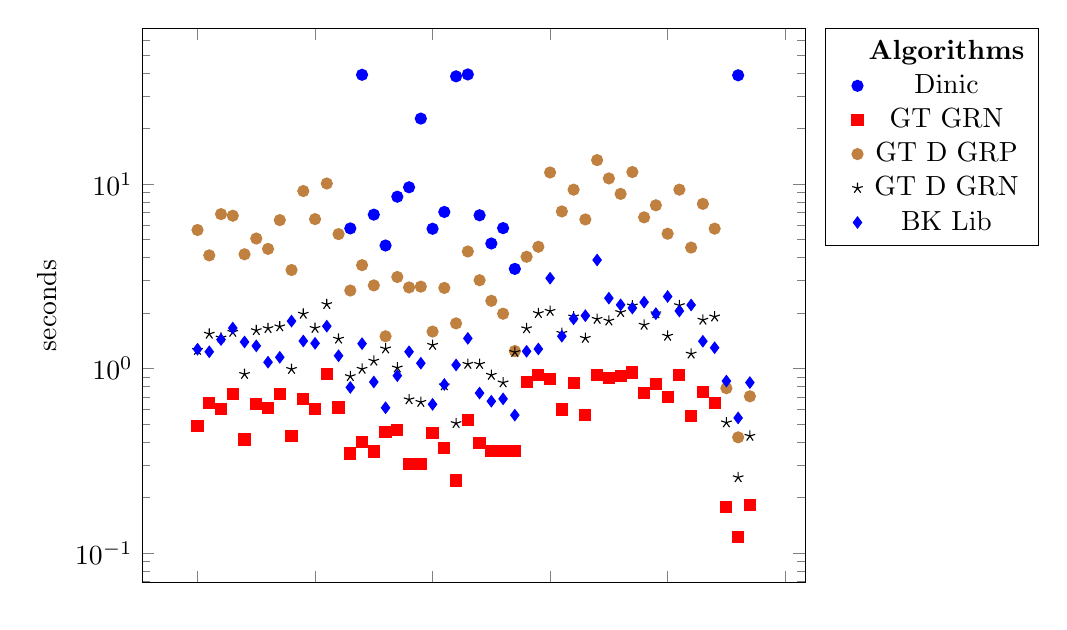
\begin{tikzpicture}
\begin{axis}[
    ylabel=seconds,ymode=log,
	symbolic x coords={BVZ-sawtooth04,BVZ-sawtooth06,BVZ-sawtooth07,BVZ-sawtooth08,BVZ-sawtooth09,BVZ-sawtooth10,BVZ-sawtooth11,BVZ-sawtooth12,BVZ-sawtooth13,BVZ-sawtooth14,BVZ-sawtooth15,BVZ-sawtooth16,BVZ-sawtooth18,BVZ-tsukuba00,BVZ-tsukuba01,BVZ-tsukuba02,BVZ-tsukuba03,BVZ-tsukuba04,BVZ-tsukuba05,BVZ-tsukuba6,BVZ-tsukuba7,BVZ-tsukuba8,BVZ-tsukuba9,BVZ-tsukuba10,BVZ-tsukuba11,BVZ-tsukuba12,BVZ-tsukuba14,BVZ-tsukuba15,BVZ-venus01,BVZ-venus02,BVZ-venus03,BVZ-venus04,BVZ-venus05,BVZ-venus06,BVZ-venus07,BVZ-venus08,BVZ-venus09,BVZ-venus10,BVZ-venus11,BVZ-venus12,BVZ-venus13,BVZ-venus14,BVZ-venus15,BVZ-venus16,BVZ-venus17,KZ2-sawtooth17,KZ2-tsukuba13,KZ2-venus19},
	xticklabels={,,},
    legend style=
    {
        legend pos=outer north east
    },
    width=10cm
]
\addlegendimage{legend image code/.code=}
\legend{\textbf{Algorithms}, Dinic, GT GRN, GT D GRP, GT D GRN, BK Lib}
\addplot[only marks, blue, mark=*] table[x=n,y=value] {%Dinic
n value
BVZ-tsukuba00	5.750836667
BVZ-tsukuba01	39.14823333
BVZ-tsukuba02	6.83006
BVZ-tsukuba03	4.645143333
BVZ-tsukuba04	8.541403333
BVZ-tsukuba05	9.609163333
BVZ-tsukuba10	39.3178
BVZ-tsukuba11	6.7765
BVZ-tsukuba12	4.763366667
BVZ-tsukuba14	5.771553333
BVZ-tsukuba15	3.468896667
BVZ-tsukuba6	22.6535
BVZ-tsukuba7	5.724696667
BVZ-tsukuba8	7.061796667
BVZ-tsukuba9	38.3952
KZ2-tsukuba13	38.90546667
};
\addplot[only marks, red, mark=square*] table[x=n,y=value] {%GT GRN
n value
BVZ-sawtooth04	0.489767333
BVZ-sawtooth06	0.650722667
BVZ-sawtooth07	0.602036667
BVZ-sawtooth08	0.728916
BVZ-sawtooth09	0.412417333
BVZ-sawtooth10	0.642597
BVZ-sawtooth11	0.610116
BVZ-sawtooth12	0.731337
BVZ-sawtooth13	0.429253333
BVZ-sawtooth14	0.683659333
BVZ-sawtooth15	0.604143
BVZ-sawtooth16	0.933819
BVZ-sawtooth18	0.614827667
BVZ-tsukuba00	0.346019
BVZ-tsukuba01	0.39826
BVZ-tsukuba02	0.355036667
BVZ-tsukuba03	0.452382667
BVZ-tsukuba04	0.462989667
BVZ-tsukuba05	0.302774
BVZ-tsukuba10	0.523340333
BVZ-tsukuba11	0.394437667
BVZ-tsukuba12	0.357265333
BVZ-tsukuba14	0.356760667
BVZ-tsukuba15	0.358245
BVZ-tsukuba6	0.30229
BVZ-tsukuba7	0.447588333
BVZ-tsukuba8	0.371264
BVZ-tsukuba9	0.247241333
BVZ-venus01	0.844272667
BVZ-venus02	0.918598
BVZ-venus03	0.873629667
BVZ-venus04	0.599272
BVZ-venus05	0.836556333
BVZ-venus06	0.559744667
BVZ-venus07	0.920171667
BVZ-venus08	0.885694
BVZ-venus09	0.912648
BVZ-venus10	0.951088333
BVZ-venus11	0.740437333
BVZ-venus12	0.821746
BVZ-venus13	0.702746333
BVZ-venus14	0.926211
BVZ-venus15	0.550986667
BVZ-venus16	0.742330333
BVZ-venus17	0.649391333
KZ2-sawtooth17	0.177902
KZ2-tsukuba13	0.12262
KZ2-venus19	0.181196667
};
\addplot[only marks, brown, mark=oplus*] table[x=n,y=value] {%GT D GRP
n value
BVZ-sawtooth04	5.637843333
BVZ-sawtooth06	4.106903333
BVZ-sawtooth07	6.87372
BVZ-sawtooth08	6.738953333
BVZ-sawtooth09	4.163056667
BVZ-sawtooth10	5.067443333
BVZ-sawtooth11	4.45305
BVZ-sawtooth12	6.378663333
BVZ-sawtooth13	3.42055
BVZ-sawtooth14	9.17015
BVZ-sawtooth15	6.45878
BVZ-sawtooth16	10.07306667
BVZ-sawtooth18	5.355506667
BVZ-tsukuba00	2.647463333
BVZ-tsukuba01	3.635553333
BVZ-tsukuba02	2.823506667
BVZ-tsukuba03	1.495733333
BVZ-tsukuba04	3.1349
BVZ-tsukuba05	2.75291
BVZ-tsukuba10	4.310993333
BVZ-tsukuba11	3.01142
BVZ-tsukuba12	2.328253333
BVZ-tsukuba14	1.98249
BVZ-tsukuba15	1.243746667
BVZ-tsukuba6	2.779606667
BVZ-tsukuba7	1.58586
BVZ-tsukuba8	2.73537
BVZ-tsukuba9	1.757243333
BVZ-venus01	4.034523333
BVZ-venus02	4.57276
BVZ-venus03	11.55953333
BVZ-venus04	7.10882
BVZ-venus05	9.328716667
BVZ-venus06	6.432303333
BVZ-venus07	13.49126667
BVZ-venus08	10.73153333
BVZ-venus09	8.848846667
BVZ-venus10	11.6229
BVZ-venus11	6.6005
BVZ-venus12	7.675843333
BVZ-venus13	5.381833333
BVZ-venus14	9.32988
BVZ-venus15	4.527093333
BVZ-venus16	7.814476667
BVZ-venus17	5.7328
KZ2-sawtooth17	0.782533333
KZ2-tsukuba13	0.42346
KZ2-venus19	0.706977667
};
\addplot[only marks, black, mark=star] table[x=n,y=value] {%GT D GRN
n value
BVZ-sawtooth04	1.257363333
BVZ-sawtooth06	1.5395
BVZ-sawtooth07	1.467783333
BVZ-sawtooth08	1.575723333
BVZ-sawtooth09	0.931440667
BVZ-sawtooth10	1.60887
BVZ-sawtooth11	1.65183
BVZ-sawtooth12	1.687383333
BVZ-sawtooth13	0.991900333
BVZ-sawtooth14	1.97617
BVZ-sawtooth15	1.65473
BVZ-sawtooth16	2.2296
BVZ-sawtooth18	1.4468
BVZ-tsukuba00	0.906884333
BVZ-tsukuba01	0.993645333
BVZ-tsukuba02	1.099296667
BVZ-tsukuba03	1.280756667
BVZ-tsukuba04	1.009479333
BVZ-tsukuba05	0.679007
BVZ-tsukuba10	1.05689
BVZ-tsukuba11	1.0557
BVZ-tsukuba12	0.921605
BVZ-tsukuba14	0.837999333
BVZ-tsukuba15	1.225756667
BVZ-tsukuba6	0.657387333
BVZ-tsukuba7	1.33941
BVZ-tsukuba8	0.807863333
BVZ-tsukuba9	0.504580667
BVZ-venus01	1.648326667
BVZ-venus02	1.992683333
BVZ-venus03	2.047933333
BVZ-venus04	1.555906667
BVZ-venus05	1.909363333
BVZ-venus06	1.461823333
BVZ-venus07	1.853596667
BVZ-venus08	1.81487
BVZ-venus09	2.017216667
BVZ-venus10	2.190356667
BVZ-venus11	1.721903333
BVZ-venus12	1.98797
BVZ-venus13	1.501023333
BVZ-venus14	2.19958
BVZ-venus15	1.20103
BVZ-venus16	1.834053333
BVZ-venus17	1.909196667
KZ2-sawtooth17	0.508664
KZ2-tsukuba13	0.256661
KZ2-venus19	0.430539333
};
\addplot[only marks, blue, mark=diamond*] table[x=n,y=value] {%BK Lib
n value
BVZ-sawtooth04	1.272543333
BVZ-sawtooth06	1.23261
BVZ-sawtooth07	1.43546
BVZ-sawtooth08	1.65753
BVZ-sawtooth09	1.39307
BVZ-sawtooth10	1.32683
BVZ-sawtooth11	1.082433333
BVZ-sawtooth12	1.150216667
BVZ-sawtooth13	1.807283333
BVZ-sawtooth14	1.409916667
BVZ-sawtooth15	1.36928
BVZ-sawtooth16	1.69699
BVZ-sawtooth18	1.172643333
BVZ-tsukuba00	0.789907667
BVZ-tsukuba01	1.363463333
BVZ-tsukuba02	0.844900667
BVZ-tsukuba03	0.612848667
BVZ-tsukuba04	0.914284667
BVZ-tsukuba05	1.232753333
BVZ-tsukuba10	1.457013333
BVZ-tsukuba11	0.736029333
BVZ-tsukuba12	0.664695333
BVZ-tsukuba14	0.684720333
BVZ-tsukuba15	0.559057667
BVZ-tsukuba6	1.068726667
BVZ-tsukuba7	0.639465
BVZ-tsukuba8	0.819790667
BVZ-tsukuba9	1.045543333
BVZ-venus01	1.240246667
BVZ-venus02	1.27637
BVZ-venus03	3.08739
BVZ-venus04	1.497496667
BVZ-venus05	1.8612
BVZ-venus06	1.934973333
BVZ-venus07	3.87581
BVZ-venus08	2.406416667
BVZ-venus09	2.214203333
BVZ-venus10	2.129076667
BVZ-venus11	2.290323333
BVZ-venus12	1.983696667
BVZ-venus13	2.456886667
BVZ-venus14	2.050246667
BVZ-venus15	2.21068
BVZ-venus16	1.405656667
BVZ-venus17	1.296033333
KZ2-sawtooth17	0.855298667
KZ2-tsukuba13	0.539781667
KZ2-venus19	0.839086
};
\end{axis}
\end{tikzpicture}
\caption{Results from the Computer Vision graphs}
\label{fig:CV_ResultsAppendix}
\end{figure}

%-----------------------------------------------------------------------------------------------------------
\clearpage


\subsection{Algorithm Running Times}
\label{AlgorithmRunningTimeSection}

\begin{figure}[h]
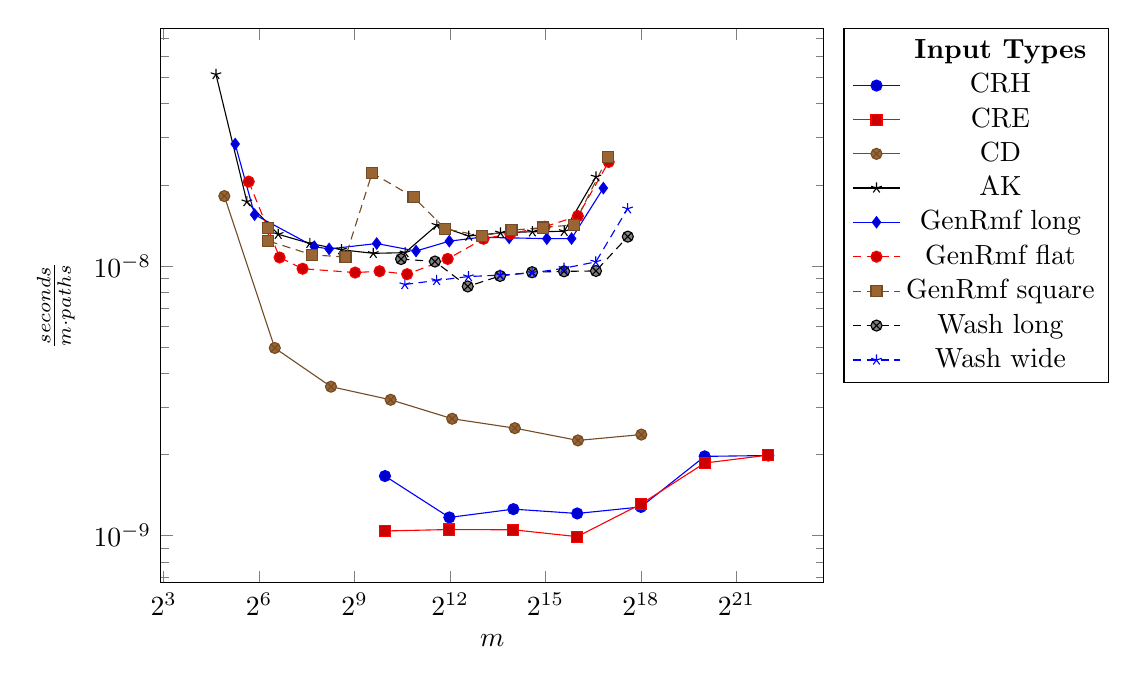
\begin{tikzpicture}
\begin{axis}[
    xlabel=$m$,ylabel=$\frac{\text{seconds}}{m\cdot \text{paths}}$,
    xmode=log,ymode=log,
    log basis x={2},
    legend style=
    {
        legend pos=outer north east
    },
    width=10cm
]
\addlegendimage{legend image code/.code=}
\legend{\textbf{Input Types}, CRH, CRE, CD, AK, GenRmf long, GenRmf flat, GenRmf square, Wash long, Wash wide}
\addplot table[x=n,y=value] {%CRH
n value
992	1.66466E-09
4032	1.16903E-09
16256	1.25451E-09
65280	1.2091E-09
261632	1.27864E-09
1047552	1.96903E-09
4192256	1.98336E-09
};
\addplot table[x=n,y=value] {%CRE
n value
992	1.0413E-09
4032	1.05426E-09
16256	1.05184E-09
65280	9.92107E-10
261632	1.31012E-09
1047552	1.85996E-09
4192256	1.99021E-09
};
\addplot table[x=n,y=value] {%CD
n value
30	1.81717E-08
90	4.96716E-09
306	3.57009E-09
1122	3.19207E-09
4290	2.71479E-09
16770	2.50517E-09
66306	2.25596E-09
263682	2.37129E-09
};
\addplot table[x=n,y=value] {%AK
n value
25	5.13295E-08
49	1.73307E-08
97	1.31136E-08
193	1.21362E-08
385	1.14906E-08
769	1.11464E-08
1537	1.12091E-08
3073	1.41778E-08
6145	1.29195E-08
12289	1.32742E-08
24577	1.34015E-08
49153	1.34511E-08
98305	2.14221E-08
};
\addplot table[x=n,y=value] {%GenRmf long
n value
38	2.83468E-08
58	1.55086E-08
213	1.17957E-08
294	1.15719E-08
828	1.21194E-08
1950	1.13672E-08
4026	1.23664E-08
7868	1.27728E-08
14840	1.27225E-08
33660	1.26353E-08
57717	1.26436E-08
115284	1.94512E-08
};
\addplot table[x=n,y=value] {%GenRmf flat
n value
51	2.05647E-08
100	1.07579E-08
165	9.77235E-09
518	9.45758E-09
882	9.56565E-09
1608	9.32887E-09
3888	1.0626E-08
8484	1.26209E-08
15232	1.31695E-08
32153	1.39854E-08
66150	1.53185E-08
129472	2.43192E-08
};
\addplot table[x=n,y=value] {%GenRmf square
n value
78	1.38184E-08
78	1.23946E-08
204	1.09934E-08
420	1.08071E-08
750	2.21376E-08
1848	1.80034E-08
3690	1.37307E-08
8268	1.29187E-08
15600	1.35717E-08
30780	1.38904E-08
60600	1.42187E-08
127968	2.5442E-08
};
\addplot table[x=n,y=value] {%Wash long
n value
1408	1.06141E-08
2944	1.03926E-08
6016	8.40057E-09
12160	9.18783E-09
24448	9.48726E-09
49024	9.55599E-09
98176	9.58903E-09
196480	1.28548E-08
};
\addplot table[x=n,y=value] {%Wash wide
n value
1528	8.54169E-09
3056	8.84407E-09
6112	9.14132E-09
12224	9.25413E-09
24448	9.42574E-09
48896	9.81213E-09
97792	1.03599E-08
195584	1.63099E-08
};
\end{axis}
\end{tikzpicture}
\caption{Edmonds and Karp performance per $m$ and the number of augmenting paths}
\label{fig:EK_runningTimeappendix}
\end{figure}



\begin{figure}[h]
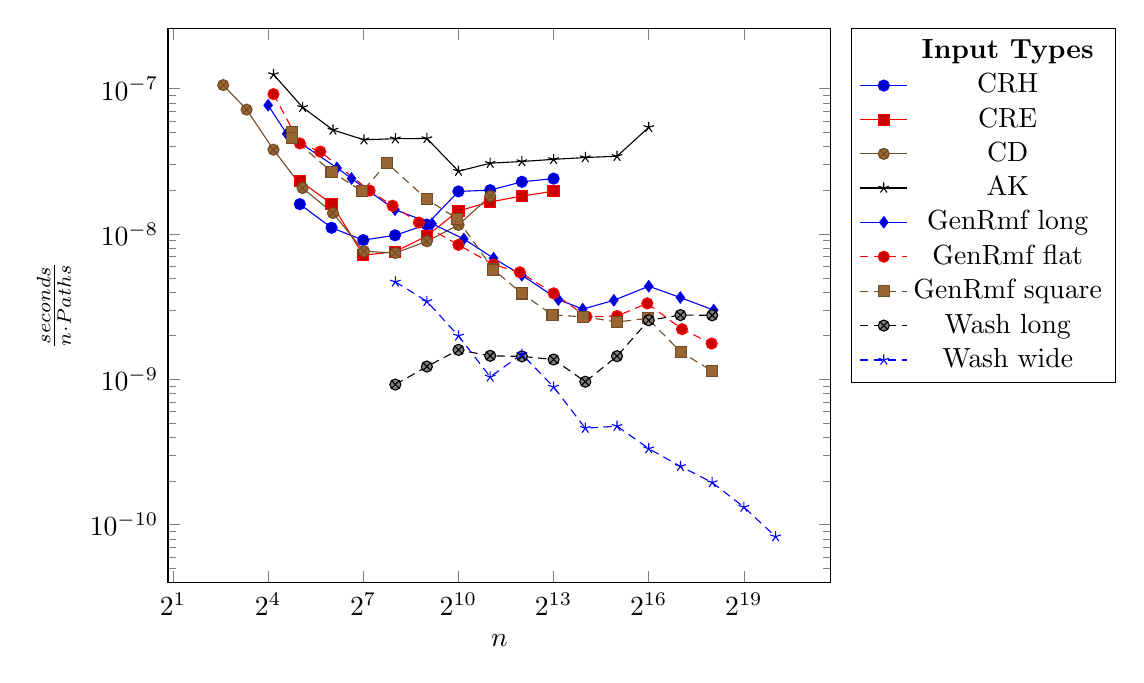
\begin{tikzpicture}
\begin{axis}[
    xlabel=$n$,ylabel=$\frac{\text{seconds}}{n\cdot \text{Paths}}$,
    xmode=log,ymode=log,
    log basis x={2},
    legend style=
    {
        legend pos=outer north east
    },
    width=10cm
]
\addlegendimage{legend image code/.code=}
\legend{\textbf{Input Types}, CRH, CRE, CD, AK, GenRmf long, GenRmf flat, GenRmf square, Wash long, Wash wide}
\addplot table[x=n,y=value] {%CRH
n value
32	1.60662E-08
64	1.10524E-08
128	9.09034E-09
256	9.8052E-09
512	1.16228E-08
1024	1.96589E-08
2048	2.00461E-08
4096	2.29003E-08
8192	2.40805E-08
};
\addplot table[x=n,y=value] {%CRE
n value
32	2.32243E-08
64	1.61998E-08
128	7.16023E-09
256	7.55879E-09
512	9.70943E-09
1024	1.44429E-08
2048	1.66357E-08
4096	1.82794E-08
8192	1.97247E-08
};
\addplot table[x=n,y=value] {%CD
n value
6	1.06002E-07
10	7.18898E-08
18	3.81028E-08
34	2.07454E-08
66	1.39579E-08
130	7.62282E-09
258	7.40559E-09
514	8.92618E-09
1026	1.1564E-08
2050	1.82553E-08
};
\addplot table[x=n,y=value] {%AK
n value
18	1.25445E-07
34	7.45452E-08
66	5.20575E-08
130	4.45512E-08
258	4.5328E-08
514	4.54889E-08
1026	2.71015E-08
2050	3.07429E-08
4098	3.15994E-08
8194	3.2674E-08
16386	3.36491E-08
32770	3.43191E-08
65538	5.42947E-08
};
\addplot table[x=n,y=value] {%GenRmf long
n value
16	7.70404E-08
24	4.90468E-08
72	2.85335E-08
99	2.41266E-08
256	1.47136E-08
575	1.17925E-08
1152	9.25426E-09
2205	6.82108E-09
4096	5.21221E-09
9100	3.54137E-09
15488	3.04506E-09
30589	3.50078E-09
65536	4.37844E-09
130682	3.65803E-09
270848	2.99932E-09
};
\addplot table[x=n,y=value] {%GenRmf flat
n value
18	9.18556E-08
32	4.20773E-08
50	3.69572E-08
147	1.99257E-08
243	1.5665E-08
432	1.19976E-08
1024	8.43176E-09
2205	6.16549E-09
3920	5.46192E-09
8214	3.90928E-09
16807	2.70144E-09
32768	2.72785E-09
63504	3.33529E-09
135531	2.21539E-09
259308	1.76556E-09
};
\addplot table[x=n,y=value] {%GenRmf square
n value
27	5.01265E-08
27	4.60135E-08
64	2.68313E-08
125	1.97155E-08
216	3.07307E-08
512	1.74072E-08
1000	1.27292E-08
2197	5.6998E-09
4096	3.90324E-09
8000	2.77607E-09
15625	2.69714E-09
32768	2.48514E-09
64000	2.62866E-09
132651	1.5397E-09
262144	1.14193E-09
};
\addplot table[x=n,y=value] {%Wash long
n value
258	9.21744E-10
514	1.22555E-09
1026	1.59596E-09
2050	1.45298E-09
4098	1.44002E-09
8194	1.37073E-09
16386	9.63818E-10
32770	1.4445E-09
65538	2.55088E-09
131074	2.77054E-09
262146	2.75927E-09
};
\addplot table[x=n,y=value] {%Wash wide
n value
258	4.6875E-09
514	3.44298E-09
1026	1.9923E-09
2050	1.03997E-09
4098	1.49151E-09
8194	8.8731E-10
16386	4.61535E-10
32770	4.76501E-10
65538	3.33716E-10
131074	2.52127E-10
262146	1.95298E-10
524290	1.32129E-10
1048578	8.27744E-11
};
\end{axis}
\end{tikzpicture}
\caption{Dinic performance per $nP$}
\label{fig:Dinic_runningTimeAppendix}
\end{figure}


\begin{figure}[h]
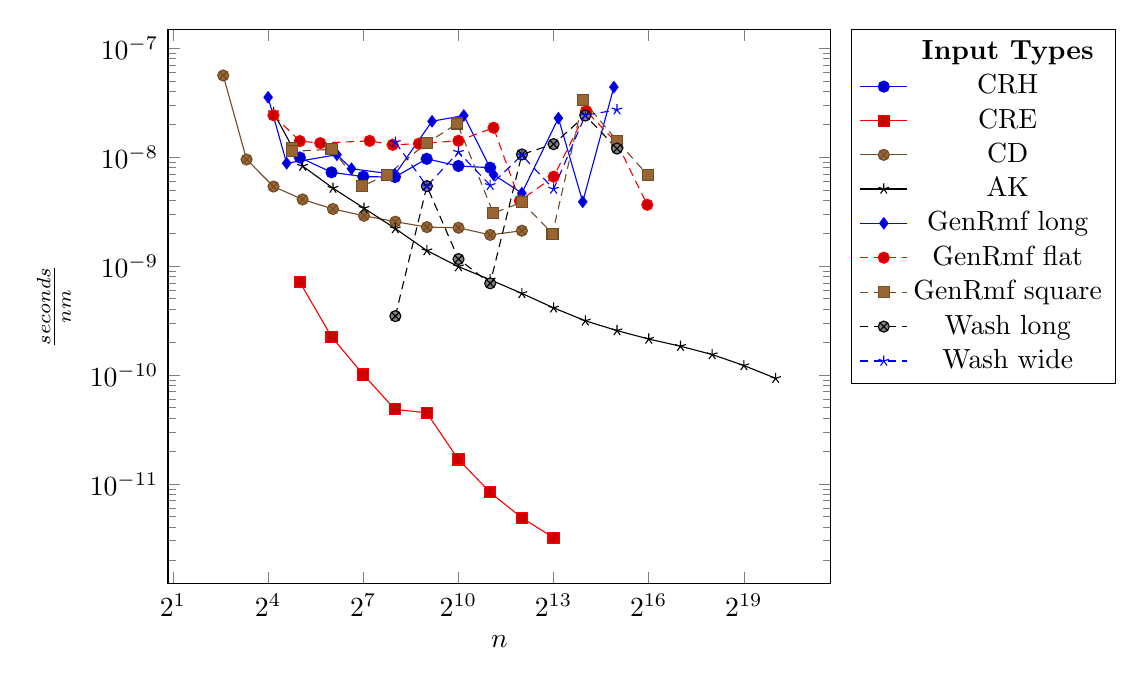
\begin{tikzpicture}
\begin{axis}[
    xlabel=$n$,ylabel=$\frac{\text{seconds}}{nm}$,
    xmode=log,ymode=log,
    log basis x={2},
    legend style=
    {
        legend pos=outer north east
    },
    width=10cm
]
\addlegendimage{legend image code/.code=}
\legend{\textbf{Input Types}, CRH, CRE, CD, AK, GenRmf long, GenRmf flat, GenRmf square, Wash long, Wash wide}
\addplot table[x=n,y=value] {%CRH
n value
32	9.90712E-09
64	7.24742E-09
128	6.61376E-09
256	6.56429E-09
512	9.63395E-09
1024	8.2859E-09
2048	7.99078E-09
};
\addplot table[x=n,y=value] {%CRE
n value
32	7.1015E-10
64	2.24209E-10
128	1.00655E-10
256	4.82229E-11
512	4.48739E-11
1024	1.67318E-11
2048	8.34562E-12
4096	4.86383E-12
8192	3.20329E-12
};
\addplot table[x=n,y=value] {%CD
n value
6	5.61416E-08
10	9.50089E-09
18	5.36295E-09
34	4.08415E-09
66	3.33572E-09
130	2.89291E-09
258	2.55076E-09
514	2.27462E-09
1026	2.24389E-09
2050	1.92973E-09
4098	2.10844E-09
};
\addplot table[x=n,y=value] {%AK
n value
18	2.56647E-08
34	8.26537E-09
66	5.18647E-09
130	3.39477E-09
258	2.20466E-09
514	1.38395E-09
1026	9.86652E-10
2050	7.47385E-10
4098	5.60005E-10
8194	4.12565E-10
16386	3.13874E-10
32770	2.54984E-10
65538	2.13448E-10
131074	1.83323E-10
262146	1.53786E-10
524290	1.21857E-10
1048578	9.30332E-11
};
\addplot table[x=n,y=value] {%GenRmf long
n value
16	3.54335E-08
24	8.77545E-09
72	1.05068E-08
99	7.81762E-09
256	6.92696E-09
575	2.13165E-08
1152	2.40867E-08
2205	6.90549E-09
4096	4.66368E-09
9100	2.27639E-08
15488	3.88656E-09
30589	4.39229E-08
};
\addplot table[x=n,y=value] {%GenRmf flat
n value
18	2.41938E-08
32	1.402E-08
50	1.34336E-08
147	1.40864E-08
243	1.29601E-08
432	1.32838E-08
1024	1.41106E-08
2205	1.8587E-08
3920	3.968E-09
8214	6.60992E-09
16807	2.63829E-08
32768	1.34006E-08
63504	3.647E-09
};
\addplot table[x=n,y=value] {%GenRmf square
n value
27	1.20752E-08
27	1.12842E-08
64	1.17888E-08
125	5.41498E-09
216	6.87753E-09
512	1.34166E-08
1000	2.0345E-08
2197	3.04784E-09
4096	3.8493E-09
8000	1.98347E-09
15625	3.31797E-08
32768	1.41112E-08
64000	6.83458E-09
};
\addplot table[x=n,y=value] {%Wash long
n value
258	3.46356E-10
514	5.40945E-09
1026	1.15649E-09
2050	6.92953E-10
4098	1.05799E-08
8194	1.31438E-08
16386	2.40597E-08
32770	1.19685E-08
};
\addplot table[x=n,y=value] {%Wash wide
n value
258	1.36924E-08
514	5.40668E-09
1026	1.11032E-08
2050	5.50623E-09
4098	1.03918E-08
8194	5.09109E-09
16386	2.41668E-08
32770	2.72197E-08
};
\end{axis}
\end{tikzpicture}
\caption{GT performance per $nm$}
\label{fig:GT_runningTimeAppendix}
\end{figure}



\begin{figure}[h]
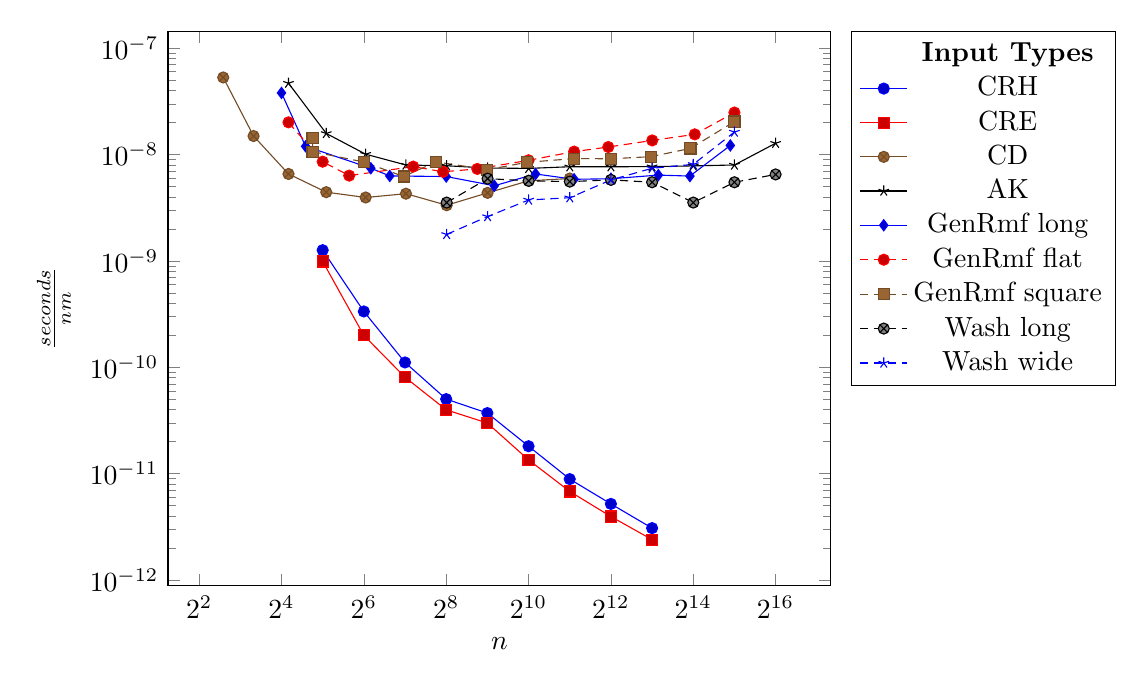
\begin{tikzpicture}
\begin{axis}[
    xlabel=$n$,ylabel=$\frac{\text{seconds}}{nm}$,
    xmode=log,ymode=log,
    log basis x={2},
    legend style=
    {
        legend pos=outer north east
    },
    width=10cm
]
\addlegendimage{legend image code/.code=}
\legend{\textbf{Input Types}, CRH, CRE, CD, AK, GenRmf long, GenRmf flat, GenRmf square, Wash long, Wash wide}
\addplot table[x=n,y=value] {%CRH
n value
32	1.26288E-09
64	3.35238E-10
128	1.11168E-10
256	5.03027E-11
512	3.71824E-11
1024	1.81421E-11
2048	8.90429E-12
4096	5.20555E-12
8192	3.0819E-12
};
\addplot table[x=n,y=value] {%CRE
n value
32	9.90013E-10
64	1.9968E-10
128	8.07477E-11
256	3.98834E-11
512	2.99502E-11
1024	1.35027E-11
2048	6.81994E-12
4096	3.96241E-12
8192	2.40243E-12
};
\addplot table[x=n,y=value] {%CD
n value
6	5.30569E-08
10	1.49299E-08
18	6.57264E-09
34	4.43056E-09
66	3.94952E-09
130	4.2887E-09
258	3.3403E-09
514	4.36561E-09
1026	5.66833E-09
2050	5.95279E-09
};
\addplot table[x=n,y=value] {%AK
n value
18	4.68876E-08
34	1.57975E-08
66	1.0078E-08
130	7.98015E-09
258	7.84601E-09
514	7.4766E-09
1026	7.41183E-09
2050	7.68286E-09
4098	7.68821E-09
8194	7.69572E-09
16386	7.82987E-09
32770	7.98256E-09
65538	1.27783E-08
};
\addplot table[x=n,y=value] {%GenRmf long
n value
16	3.79906E-08
24	1.19665E-08
72	7.4366E-09
99	6.29532E-09
256	6.21655E-09
575	5.09247E-09
1152	6.56912E-09
2205	5.85557E-09
4096	5.92566E-09
9100	6.41111E-09
15488	6.27912E-09
30589	1.21796E-08
};
\addplot table[x=n,y=value] {%GenRmf flat
n value
18	2.00808E-08
32	8.57161E-09
50	6.33991E-09
147	7.7075E-09
243	6.89168E-09
432	7.32937E-09
1024	8.83296E-09
2205	1.06628E-08
3920	1.1773E-08
8214	1.3578E-08
16807	1.54848E-08
32768	2.48237E-08
};
\addplot table[x=n,y=value] {%GenRmf square
n value
27	1.43953E-08
27	1.06515E-08
64	8.51412E-09
125	6.22088E-09
216	8.53572E-09
512	7.21217E-09
1000	8.45903E-09
2197	9.16498E-09
4096	9.1337E-09
8000	9.54867E-09
15625	1.14186E-08
32768	2.04167E-08
};
\addplot table[x=n,y=value] {%Wash long
n value
258	3.53846E-09
514	5.93937E-09
1026	5.66374E-09
2050	5.56832E-09
4098	5.78294E-09
8194	5.49482E-09
16386	3.53918E-09
32770	5.49036E-09
65538	6.50731E-09
};
\addplot table[x=n,y=value] {%Wash wide
n value
258	1.77663E-09
514	2.61444E-09
1026	3.74229E-09
2050	3.93122E-09
4098	5.77718E-09
8194	7.43357E-09
16386	8.0869E-09
32770	1.62903E-08
};
\end{axis}
\end{tikzpicture}
\caption{GT GRC performance per $nm$}
\label{fig:GT_GRC_runningTimeAppendix}
\end{figure}



\begin{figure}[h]
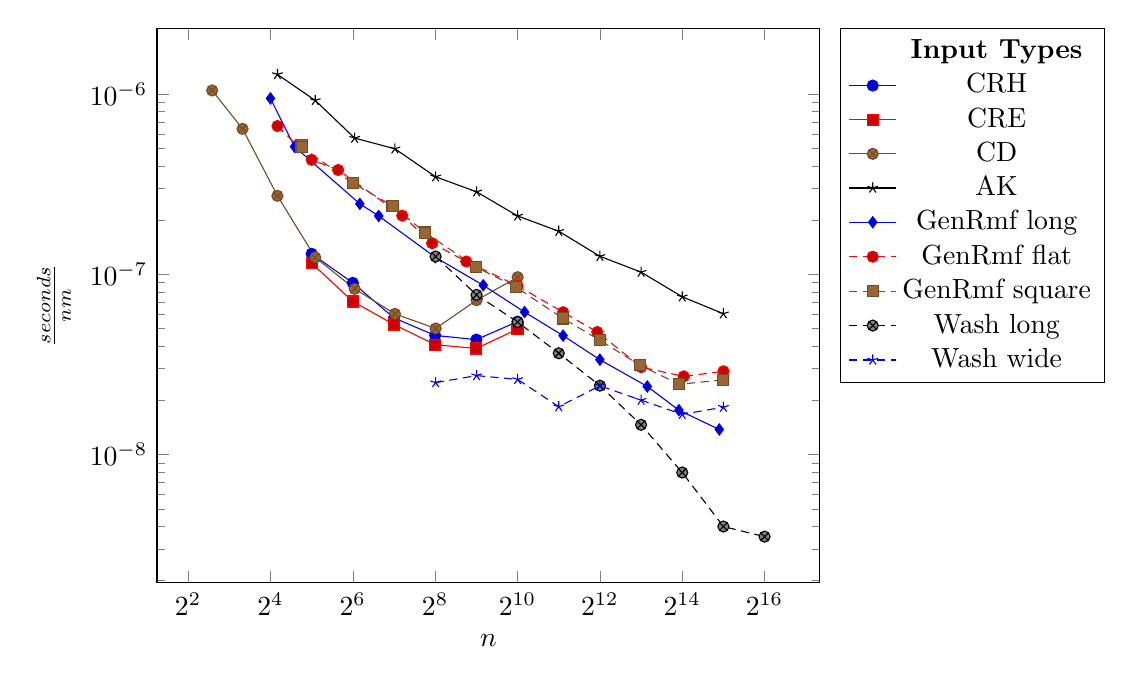
\begin{tikzpicture}
\begin{axis}[
    xlabel=$n$,ylabel=$\frac{\text{seconds}}{nm}$,
    xmode=log,ymode=log,
    log basis x={2},
    legend style=
    {
        legend pos=outer north east
    },
    width=10cm
]
\addlegendimage{legend image code/.code=}
\legend{\textbf{Input Types}, CRH, CRE, CD, AK, GenRmf long, GenRmf flat, GenRmf square, Wash long, Wash wide}
\addplot table[x=n,y=value] {%CRH
n value
32	1.30007E-07
64	8.96393E-08
128	5.72588E-08
256	4.57896E-08
512	4.343E-08
1024	5.46341E-08
};
\addplot table[x=n,y=value] {%CRE
n value
32	1.15261E-07
64	7.06504E-08
128	5.26847E-08
256	4.06767E-08
512	3.87895E-08
1024	4.96835E-08
};
\addplot table[x=n,y=value] {%CD
n value
6	1.04695E-06
10	6.41125E-07
18	2.72502E-07
34	1.24094E-07
66	8.30602E-08
130	6.03361E-08
258	5.00513E-08
514	7.18575E-08
1026	9.63497E-08
};
\addplot table[x=n,y=value] {%AK
n value
18	1.28447E-06
34	9.22187E-07
66	5.69731E-07
130	4.97013E-07
258	3.47541E-07
514	2.8686E-07
1026	2.10738E-07
2050	1.73426E-07
4098	1.25893E-07
8194	1.0284E-07
16386	7.50472E-08
32770	6.04413E-08
};
\addplot table[x=n,y=value] {%GenRmf long
n value
16	9.46111E-07
24	5.10492E-07
72	2.45994E-07
99	2.1071E-07
256	1.24506E-07
575	8.69615E-08
1152	6.17645E-08
2205	4.56919E-08
4096	3.36001E-08
9100	2.38667E-08
15488	1.76328E-08
30589	1.37729E-08
};
\addplot table[x=n,y=value] {%GenRmf flat
n value
18	6.64723E-07
32	4.31634E-07
50	3.79102E-07
147	2.11565E-07
243	1.48769E-07
432	1.17769E-07
1024	8.63694E-08
2205	6.16427E-08
3920	4.78561E-08
8214	3.05494E-08
16807	2.71511E-08
32768	2.89605E-08
};
\addplot table[x=n,y=value] {%GenRmf square
n value
27	5.215E-07
27	5.08105E-07
64	3.20687E-07
125	2.39996E-07
216	1.7053E-07
512	1.09497E-07
1000	8.49219E-08
2197	5.68963E-08
4096	4.30881E-08
8000	3.13326E-08
15625	2.45354E-08
32768	2.59762E-08
};
\addplot table[x=n,y=value] {%Wash long
n value
258	1.25491E-07
514	7.69137E-08
1026	5.43358E-08
2050	3.6474E-08
4098	2.41164E-08
8194	1.46208E-08
16386	7.95112E-09
32770	3.98875E-09
65538	3.50499E-09
};
\addplot table[x=n,y=value] {%Wash wide
n value
258	2.5073E-08
514	2.74194E-08
1026	2.6114E-08
2050	1.84365E-08
4098	2.40671E-08
8194	2.00366E-08
16386	1.6713E-08
32770	1.83213E-08
};
\end{axis}
\end{tikzpicture}
\caption{GR performance per $nm$}
\label{fig:GR_runningTimeAppendix}
\end{figure}

\end{subappendices}